
% This LaTeX was auto-generated from MATLAB code.
% To make changes, update the MATLAB code and republish this document.

\documentclass{article}
\usepackage{graphicx}
\usepackage{color}

\sloppy
\definecolor{lightgray}{gray}{0.5}
\setlength{\parindent}{0pt}

\begin{document}

    
    
\section*{Guaranteed Automatic Integration Library (GAIL) Version 2.3.1 Documentation}

\begin{par}
GAIL (Guaranteed Automatic Integration Library) is created, developed, and maintained by Fred Hickernell (Illinois Institute of Technology), Sou-Cheng Choi (IIT), Yuhan Ding (IIT), Lan Jiang (IIT), Lluis Antoni Jimenez Rugama (IIT), Xin Tong (University of Illinois at Chicago), Yizhi Zhang (IIT), and Xuan Zhou (IIT).
\end{par} \vspace{1em}
\begin{par}
GAIL is a suite of algorithms for integration problems in one, many, and infinite dimensions, and whose answers are guaranteed to be correct.
\end{par} \vspace{1em}

\subsection*{Contents}

\begin{itemize}
\setlength{\itemsep}{-1ex}
   \item Introduction
   \item Functions
   \item Demos
   \item Website
   \item GAIL License
   \item Developed by
   \item Downloads
   \item Requirements
   \item Documentation
   \item General Usage Notes
   \item Installation Instruction
   \item Tests
   \item Known Bugs
   \item Contact Information
   \item Acknowledgements
   \item Release Notes
   \item Major changes in algorithms
   \item Major changes in publications
   \item Major changes in documentation
   \item Major changes in tests
   \item Functions
   \item 1-D approximation
   \item 1-D integration
   \item 1-D minimization
   \item Higher dimensional integration
   \item GAIL Demos
   \item 1-D approximation
   \item 1-D minimization
   \item 1-D integration
   \item Higher dimensional integration
   \item funappx\_g
   \item Syntax
   \item Description
   \item Guarantee
   \item Examples
   \item See Also
   \item References
   \item funmin\_g
   \item Syntax
   \item Description
   \item Guarantee
   \item Examples
   \item See Also
   \item References
   \item integral\_g
   \item Syntax
   \item Description
   \item Guarantee
   \item Examples
   \item See Also
   \item References
   \item meanMC\_g
   \item Syntax
   \item Description
   \item Guarantee
   \item Examples
   \item See Also
   \item References
   \item meanMC\_CLT
   \item Syntax
   \item Description
   \item Examples
   \item References
   \item Syntax
   \item Description
   \item Guarantee
   \item Examples
   \item See Also
   \item References
   \item cubLattice\_g
   \item Syntax
   \item Description
   \item Guarantee
   \item Examples
   \item See Also
   \item References
   \item cubSobol\_g
   \item Syntax
   \item Description
   \item Guarantee
   \item Examples
   \item See Also
   \item References
   \item cubBayesLattice\_g
   \item Syntax
   \item Description
   \item Guarantee
   \item Examples
   \item See Also
   \item References
   \item Demos for funappx\_g
   \item Approximate a highly fluctuating curve using \textbf{funappx\_g}
   \item Function definition
   \item Function approximation
   \item Plots of the function and approximant
   \item Plot of the approximation errors
   \item A slightly different example
   \item A workaround
   \item A better way
   \item References
   \item A GUI (graphical user interface) for \textbf{funappx\_g}
   \item Function definition
   \item Function Approximation
   \item Process to Generate Grid Points
   \item References
   \item Demos for funmin\_g
   \item Find the minimum of a highly oscillating curve using \textbf{funmin\_g}
   \item Function definition
   \item Function minimization
   \item Plots of the function and its minimum
   \item A fix
   \item References
   \item Compare \textbf{funmin\_g} with \textbf{fminbnd}
   \item Function definition
   \item Function minimization
   \item Plot of the function and minima
   \item References
   \item Demos for integral\_g
   \item Integrate a spiky function using \textbf{integral\_g}
   \item Function definition
   \item Plot of the spiky function
   \item Integral approximation
   \item Compute approximation errors
   \item References
   \item Demos for meanMC\_g
   \item Demos for cubMC\_g
   \item Estimation of normal probabilities by \textbf{cubSobol\_g} and \textbf{cubMC\_g}
   \item Basic integration parameters set up
   \item First test: \ensuremath{\backslash}(\ensuremath{\backslash}Sigma=I\_d\ensuremath{\backslash})
   \item Second test: \ensuremath{\backslash}(\ensuremath{\backslash}Sigma=0.4I\_d + 0.6\ensuremath{\backslash}bf\{1\}\ensuremath{\backslash}bf\{1\}\^{}T\ensuremath{\backslash})
   \item Third test: \ensuremath{\backslash}(\ensuremath{\backslash}Sigma=0.4I\_d + 0.6\ensuremath{\backslash}bf\{1\}\ensuremath{\backslash}bf\{1\}\^{}T\ensuremath{\backslash})
   \item Appendix: Auxiliary function definitions
   \item References
\end{itemize}


\subsection*{Introduction}

\begin{par}

\end{par} \vspace{1em}


\subsection*{Functions}

\begin{par}

\end{par} \vspace{1em}


\subsection*{Demos}

\begin{par}

\end{par} \vspace{1em}


\subsection*{Website}

\begin{par}
For more information about GAIL, visit \begin{verbatim}Gailteam\end{verbatim}
\end{par} \vspace{1em}


\subsection*{GAIL License}

\begin{verbatim}
%Copyright � 2019, Illinois Institute of Technology. All rights reserved.
%
% Redistribution and use in source and binary forms, with or without
% modification, are permitted provided that the following conditions are
% met:
%
%   * Redistributions of source code must retain the above copyright
%     notice, this list of conditions and the following disclaimer.
%
%   * Redistributions in binary form must reproduce the above copyright
%     notice, this list of conditions and the following disclaimer in the
%     documentation and/or other materials provided with the distribution.
%
%   * Neither the name of Illinois Institute of Technology nor the names of
%     its contributors may be used to endorse or promote products derived
%     from this software without specific prior written permission.
%
% THIS SOFTWARE IS PROVIDED BY THE COPYRIGHT HOLDER AND CONTRIBUTORS
% "AS IS" AND WITHOUT ANY WARRANTY OF ANY KIND, WHETHER EXPRESS, IMPLIED,
% STATUTORY OR OTHERWISE, INCLUDING WITHOUT LIMITATION WARRANTIES OF
% MERCHANTABILITY, FITNESS FOR A PARTICULAR USE AND NON-INFRINGEMENT, ALL
% OF WHICH ARE HEREBY EXPRESSLY DISCLAIMED. MOREOVER, THE USER OF THE
% SOFTWARE UNDERSTANDS AND AGREES THAT THE SOFTWARE MAY CONTAIN BUGS,
% DEFECTS, ERRORS AND OTHER PROBLEMS THAT COULD CAUSE SYSTEM FAILURES, AND
% ANY USE OF THE SOFTWARE SHALL BE AT USER?S OWN RISK. THE COPYRIGHT
% HOLDERS AND CONTRIBUTORS MAKES NO REPRESENTATION THAT THEY WILL ISSUE
% UPDATES OR ENHANCEMENTS TO THE SOFTWARE.
%
% IN NO EVENT WILL THE COPYRIGHT HOLDER OR CONTRIBUTORS BE LIABLE FOR ANY
% DIRECT, INDIRECT, SPECIAL, INCIDENTAL, CONSEQUENTIAL, EXEMPLARY OR
% PUNITIVE DAMAGES, INCLUDING, BUT NOT LIMITED TO, DAMAGES FOR INTERRUPTION
% OF USE OR FOR LOSS OR INACCURACY OR CORRUPTION OF DATA, LOST PROFITS, OR
% COSTS OF PROCUREMENT OF SUBSTITUTE GOODS OR SERVICES, HOWEVER CAUSED
% (INCLUDING BUT NOT LIMITED TO USE, MISUSE, INABILITY TO USE, OR
% INTERRUPTED USE) AND UNDER ANY THEORY OF LIABILITY, INCLUDING BUT NOT
% LIMITED TO CONTRACT, STRICT LIABILITY, OR TORT (INCLUDING NEGLIGENCE OR
% OTHERWISE) ARISING IN ANY WAY OUT OF THE USE OF THIS SOFTWARE, EVEN IF
% ADVISED OF THE POSSIBILITY OF SUCH DAMAGE AND WHETHER OR NOT THE
% COPYRIGHT HOLDER AND CONTRIBUTORS WAS OR SHOULD HAVE BEEN AWARE OR
% ADVISED OF THE POSSIBILITY OF SUCH DAMAGE OR FOR ANY CLAIM ALLEGING
% INJURY RESULTING FROM ERRORS, OMISSIONS, OR OTHER INACCURACIES IN THE
% SOFTWARE OR DESTRUCTIVE PROPERTIES OF THE SOFTWARE.  TO THE EXTENT THAT
% THE LAWS OF ANY JURISDICTIONS DO NOT ALLOW THE FOREGOING EXCLUSIONS AND
% LIMITATION, THE USER OF THE SOFTWARE AGREES THAT DAMAGES MAY BE
% DIFFICULT, IF NOT IMPOSSIBLE TO CALCULATE, AND AS A RESULT, SAID USER HAS
% AGREED THAT THE MAXIMUM LIABILITY OF THE COPYRITGHT HOLDER AND
% CONTRIBUTORS SHALL NOT EXCEED US$100.00.
%
% THE USER OF THE SOFTWARE ACKNOWLEDGES THAT THE SOFTWARE IS BEING PROVIDED
% WITHOUT CHARGE, AND AS A RESULT, THE USER, ACKNOWLEDGING THAT HE OR SHE
% HAS READ THE SAME, AGREES THAT THE FOREGOING LIMITATIONS AND RESTRICTIONS
% REPRESENT A REASONABLE ALLOCATION OF RISK.%% Guaranteed Automatic Integration Library (GAIL)
%
% GAIL Version 2.3.1, 2020.
%
% See LICENSE.m for copyright and disclaimer. Refer to ReleaseNotes.m for
% what is new in this version.
%
% GAIL is a suite of algorithms for integration problems in one and many
% dimensions, and whose answers are guaranteed to be correct.
%
%
%
\end{verbatim}


\subsection*{Developed by}

\begin{par}
Fred Hickernell, Sou-Cheng Choi, and their collaborators including Yuhan Ding, Lan Jiang, Lluis Antoni Jimenez Rugama, Da Li, Jagadeeswaran Rathinavel, Kan Zhang, Yizhi Zhang, and Xuan Zhou, Department of Applied Mathematics, Illinois Institute of Technology (IIT) and  Xin Tong, Department of Mathematics, Statistics, and Computer Science, University of Illinois at Chicago. We thank the contributions of Francisco Hernandez, Cu Hauw Hung, Yueyi Li, Xincheng Sheng, Xiaoyang Zhao, Tianci Zhu, and the IIT classes of SCI 498 Adaptive Monte Carlo Algorithms with Applications to Financial Risk Management, Summer 2016; MATH 491 Reading \& Research, Summer 2015; SCI 498/MATH 491 Computational Social Sciences, Summer 2016; MATH 491-195 Solving Problems in the Social Sciences Using Tools from Computational Mathematics and Statistics, Summer 2015; Math 573 Reliable Mathematical Software, Fall 2013.
\end{par} \vspace{1em}
\begin{par}
Please cite the following software, papers, and materials:
\end{par} \vspace{1em}
\begin{par}
Sou-Cheng T. Choi, "MINRES-QLP Pack and Reliable Reproducible Research via Supportable Scientific Software," Journal of Open Research Software, Volume 2, Number 1, e22, pp. 1-7, 2014. (describes principles of Reliable Reproducible Research and Supportable Scientific Software)
\end{par} \vspace{1em}
\begin{par}
Sou-Cheng T. Choi, Yuhan Ding, Fred J. Hickernell, Lan Jiang, Lluis Antoni Jimenez Rugama, Da Li, Jagadeeswaran Rathinavel, Xin Tong, Kan Zhang, Yizhi Zhang, and Xuan Zhou, GAIL: Guaranteed Automatic Integration Library (Version 2.3.1) [MATLAB Software], 2020. Available from \begin{verbatim}http://gailgithub.github.io/GAIL_Dev/\end{verbatim} (this software)
\end{par} \vspace{1em}
\begin{par}
Sou-Cheng T. Choi, Yuhan Ding, Fred J. Hickernell, Xin Tong, "Local Adaption for Approximation and Minimization of Univariate Functions," Journal of Complexity 40, pp. 17-33, 2017. (describes \textbf{funappx\_g.m} and \textbf{funmin\_g.m})
\end{par} \vspace{1em}
\begin{par}
Sou-Cheng T. Choi and Fred J. Hickernell, "IIT MATH-573 Reliable Mathematical Software" [Course Slides], Illinois Institute of Technology, Chicago, IL, 2013. Available from \begin{verbatim}http://gailgithub.github.io/GAIL_Dev/\end{verbatim} (develops practices of Reliable Reproducible Research and Supportable Scientific Software)
\end{par} \vspace{1em}
\begin{par}
Nicholas Clancy, Yuhan Ding, Caleb Hamilton, Fred J. Hickernell, and Yizhi Zhang, "The Cost of Deterministic, Adaptive, Automatic Algorithms: Cones, Not Balls," Journal of Complexity 30, pp. 21-45, 2014. (describes deprecated \textbf{integralPenalty\_g.m} and deprecated \textbf{funappxtau\_g.m})
\end{par} \vspace{1em}
\begin{par}
Yuhan Ding, "Guaranteed Adaptive Univariate Function Approximation," PhD thesis, Illinois Institute of Technology, 2015. (describes deprecated \textbf{funappxPenalty\_g.m})
\end{par} \vspace{1em}
\begin{par}
Fred J. Hickernell, Lan Jiang, Yuewei Liu, and Art B. Owen, "Guaranteed conservative fixed width confidence intervals via Monte Carlo sampling," Monte Carlo and Quasi-Monte Carlo Methods 2012 (J. Dick, F. Y. Kuo, G. W. Peters, and I. H. Sloan, eds.), Springer-Verlag, Berlin, pp. 105-128, 2014. (describes \textbf{meanMC\_g.m} and \textbf{cubMC\_g.m})
\end{par} \vspace{1em}
\begin{par}
Fred J. Hickernell and Lluis Antoni Jimenez Rugama, "Reliable adaptive cubature using digital sequences", Monte Carlo and Quasi-Monte Carlo Methods: MCQMC, Leuven, Belgium, April 2014 (R. Cools and D. Nuyens, eds.), Springer Proceedings in Mathematics and Statistics, vol. 163, Springer-Verlag, Berlin, 2016, arXiv:1410.8615 [math.NA], pp. 367-383. (describes \textbf{cubSobol\_g.m})
\end{par} \vspace{1em}
\begin{par}
Fred J. Hickernell, Lluis Antoni Jimenez Rugama, and Da Li, "Adaptive quasi-Monte Carlo methods, 2017+, submitted for publication, arXiv:1702.01491 [math.NA].
\end{par} \vspace{1em}
\begin{par}
Fred J. Hickernell, Martha Razo, and Sunny Yun, "Reliable Adaptive Numerical Integration", 2015+, working. (describes \textbf{integral\_g.m})
\end{par} \vspace{1em}
\begin{par}
Lan Jiang, Guaranteed Adaptive Monte Carlo Methods for Estimating Means of Random Variables, PhD Thesis, Illinois Institute of Technology, 2016. (describes \textbf{meanMC\_g.m} and \textbf{cubMC\_g.m})
\end{par} \vspace{1em}
\begin{par}
Lluis Antoni Jimenez Rugama and Fred J. Hickernell, "Adaptive multidimensional integration based on rank-1 lattices," Monte Carlo and Quasi-Monte Carlo  Methods: MCQMC, Leuven, Belgium, April 2014 (R. Cools and D. Nuyens, eds.), Springer Proceedings in Mathematics and Statistics, vol. 163, Springer-Verlag, Berlin, 2016, arXiv:1411.1966, pp. 407-422. (describes cubLattice\_g.m)
\end{par} \vspace{1em}
\begin{par}
Daniel S. Katz, Sou-Cheng T. Choi, Hilmar Lapp, Ketan Maheshwari, Frank Loffler, Matthew Turk, Marcus D. Hanwell, Nancy Wilkins-Diehr, James Hetherington, James Howison, Shel Swenson, Gabrielle D. Allen, Anne C. Elster, Bruce Berriman, Colin Venters, "Summary of the First Workshop On Sustainable Software for Science: Practice and Experiences (WSSSPE1)," Journal of Open Research Software, Volume 2, Number 1, e6, pp. 1-21, 2014. (discusses practice and challenges in Sustainable Software for Science)
\end{par} \vspace{1em}
\begin{par}
Daniel S. Katz, Sou-Cheng T. Choi, Nancy Wilkins-Diehr, Neil Chue Hong, Colin C. Venters, James Howison, Frank J. Seinstra, Matthew Jones, Karen Cranston, Thomas L. Clune,  Miguel de Val-Borro, and Richard Littauer, "Report on the Second Workshop on Sustainable Software for Science: Practice and Experiences (WSSSPE2)," Journal of Open Research Software, Volume 4, Number 1, e7, 2016. (discusses practice and challenges in Sustainable Software for Science)
\end{par} \vspace{1em}
\begin{par}
Daniel S. Katz, Sou-Cheng T. Choi, Kyle E. Niemeyer, James Hetherington, Frank L\{offler, Dan Gunter, Ray Idaszak, Steven R. Brandt, Mark A. Miller, Sandra Gesing, Nick D. Jones, Nic Weber, Suresh Marru, Gabrielle Allen, Birgit Penzenstadler, Colin C. Venters, Ethan Davis, Lorraine Hwang, Ilian Todorov, Abani Patra, and Miguel de Val-Borro, "Report on the Third Workshop on Sustainable Software for Science: Practice and Experiences (WSSSPE3)," Journal of Open Research Software, Volume 4, Number 1, e37, 2016. (discusses practice and challenges in Sustainable Software for Science)
\end{par} \vspace{1em}
\begin{par}
Da Li, "Reliable Quasi-Monte Carlo with Control Variates," Master's thesis, Illinois Institute of Technology, 2016. (describes \textbf{cubSobol\_g.m} for control variates)
\end{par} \vspace{1em}
\begin{par}
Arfon M. Smith, Daniel S. Katz, Kyle E. Niemeyer, and FORCE11 Software Citation Working Group, "Software citation principles," PeerJ Computer Science, Volume 2, e86, 2016. (motivates research software citation)
\end{par} \vspace{1em}
\begin{par}
Xin Tong, "A Guaranteed, Adaptive, Automatic Algorithm for Univariate Function Minimization," MS thesis, Illinois Institute of Technology, 2014. (describes deprecated funmin01\_g.m)
\end{par} \vspace{1em}


\subsection*{Downloads}

\begin{par}
GAIL can be downloaded from \begin{verbatim}http://gailgithub.github.io/GAIL_Dev/\end{verbatim}.
\end{par} \vspace{1em}
\begin{par}
Alternatively, you can get a local copy of the GAIL repository with this command:
\end{par} \vspace{1em}
\begin{verbatim}git clone https://github.com/GailGithub/GAIL_Dev.git\end{verbatim}


\subsection*{Requirements}

\begin{par}
You will need to install MATLAB 7 or a later version.
\end{par} \vspace{1em}


\subsection*{Documentation}

\begin{par}
Detailed documentation is available at GAIL\_Matlab/Documentation.
\end{par} \vspace{1em}


\subsection*{General Usage Notes}

\begin{par}
GAIL Version 2.3.1 includes the following eight algorithms:
\end{par} \vspace{1em}
\begin{par}
1.  \textbf{funappx\_g}: One-dimensional function approximation on bounded interval
\end{par} \vspace{1em}
\begin{par}
2.  \textbf{funmin\_g}: global minimum value of univariate function on a closed interval
\end{par} \vspace{1em}
\begin{par}
3.  \textbf{integral\_g}: One-dimensional integration on bounded interval
\end{par} \vspace{1em}
\begin{par}
4.  \textbf{meanMC\_g}: Monte Carlo method for estimating mean of a random variable
\end{par} \vspace{1em}
\begin{par}
5.  \textbf{cubMC\_g}: Monte Carlo method for numerical multiple integration
\end{par} \vspace{1em}
\begin{par}
6.  \textbf{cubSobol\_g}: Quasi-Monte Carlo method using Sobol' cubature for d-dimensional integration
\end{par} \vspace{1em}
\begin{par}
7.  \textbf{cubLattice\_g}: Quasi-Monte Carlo method using rank-1 Lattices cubature for d-dimensional integration
\end{par} \vspace{1em}
\begin{par}
8.  \textbf{meanMC\_CLT}: Monte Carlo method with Central Limit Theorem (CLT) confidence intervals for estimating mean of a random variable
\end{par} \vspace{1em}


\subsection*{Installation Instruction}

\begin{par}
1.  Unzip the contents of the zip file to a directory and maintain the     existing directory and subdirectory structure. (Please note: If you     install into the "toolbox" subdirectory of the MATLAB program     hierarchy, you will need to click the button "Update toolbox path     cache" from the File/Preferences... dialog in MATLAB.)
\end{par} \vspace{1em}
\begin{par}
2.  In MATLAB, add the GAIL directory to your path. This can be done     by running "GAIL\_Install.m".  Alternatively, this can be done by     selecting "File/Set Path..." from the main or Command window     menus, or with the command "pathtool". We recommend that you     select the "Save" button on this dialog so that GAIL is on the     path automatically in future MATLAB sessions.
\end{par} \vspace{1em}
\begin{par}
3.  To check if you have installed GAIL successfully, type "help     funappx\_g" to see if its documentation shows up.
\end{par} \vspace{1em}
\begin{par}
Alternatively, you could do this:
\end{par} \vspace{1em}
\begin{par}
1.  Download DownloadInstallGail\_2\_3.m and put it where you want     GAIL to be installed.
\end{par} \vspace{1em}
\begin{par}
2.  Execute it in MATLAB.
\end{par} \vspace{1em}
\begin{par}
To uninstall GAIL, execute "GAIL\_Uninstall".
\end{par} \vspace{1em}
\begin{par}
To reinstall GAIL, execute "GAIL\_Install".
\end{par} \vspace{1em}


\subsection*{Tests}

\begin{par}
We provide quick doctests for each of the functions above. To run doctests in funappx\_g, for example, issue the command doctest funappx\_g.
\end{par} \vspace{1em}
\begin{par}
We also provide unit tests for MATLAB version 8 or later. To run unit tests for funmin\_g, for instance, execute run(ut\_funmin\_g).
\end{par} \vspace{1em}


\subsection*{Known Bugs}

\begin{par}
None.
\end{par} \vspace{1em}


\subsection*{Contact Information}

\begin{par}
Please send any queries, questions, or comments to \begin{verbatim}gail-users@googlegroups.com\end{verbatim} or visit our project website: \begin{verbatim}http://gailgithub.github.io/GAIL_Dev/\end{verbatim}
\end{par} \vspace{1em}


\subsection*{Acknowledgements}

\begin{par}
Our work was supported in part by grants from the National Science Foundation under grant NSF-DMS-1115392, and the Office of Advanced Scientific Computing Research, Office of Science, U.S. Department of Energy, under contract DE-AC02-06CH11357.
\end{par} \vspace{1em}


\subsection*{Release Notes}

\begin{par}
GAIL Version 2.3.1, 2020.
\end{par} \vspace{1em}


\subsection*{Major changes in algorithms}

\begin{par}
We have a new algorithm called \textbf{meanMC\_CLT}. In addition, all algorithms in version 2.1 are improved with reduced computational complexity and some new features. For example, funappx\_g and funmin\_g are locally adaptive; our three multidimensional integration algorithms (\textbf{cubMC\_g}, \textbf{cubLattice\_g}, and \textbf{cubSobol\_g}) may take the probability measure uniform sphere in addition to uniform hyperbox and Gaussian. The directory Algorithms is reorganized with new subfolders to group algorithms and object classes by their shared functionalities. We deprecated \textbf{funappx\_g}, \textbf{funmin\_g}, and integral\_g in version 2.1 and renamed them in this version as \textbf{funappxPenalty\_g}, \textbf{funminPenalty\_g}, and \textbf{integralPenalty\_g}, respectively. Lastly, \textbf{meanMCBer\_g} in version 2.1 is removed.
\end{par} \vspace{1em}


\subsection*{Major changes in publications}

\begin{par}
In the folder "Papers", we include currently working and recently published research articles related to our core algorithms. In addition, we have included nine PhD or MS theses relevant to our research areas. For theses and published papers, we included the PDF files of the articles as well as MATLAB scripts for reproducing key figures, tables, and numerical results in the papers.
\end{par} \vspace{1em}


\subsection*{Major changes in documentation}

\begin{par}
We continue to release both PDF and searchable HTML documentation for GAIL in MATLAB.  In addition, we have added more than a half dozen demos for our algorithms.
\end{par} \vspace{1em}


\subsection*{Major changes in tests}

\begin{par}
We continue to conduct automated nightly tests and weekly long tests on our own server.
\end{par} \vspace{1em}


\subsection*{Functions}



\subsection*{1-D approximation}

\begin{par}

\end{par} \vspace{1em}


\subsection*{1-D integration}

\begin{par}

\end{par} \vspace{1em}


\subsection*{1-D minimization}

\begin{par}

\end{par} \vspace{1em}


\subsection*{Higher dimensional integration}

\begin{par}

\end{par} \vspace{1em}
\begin{par}

\end{par} \vspace{1em}
\begin{par}

\end{par} \vspace{1em}
\begin{par}

\end{par} \vspace{1em}
\begin{par}

\end{par} \vspace{1em}


\subsection*{GAIL Demos}



\subsection*{1-D approximation}

\begin{par}

\end{par} \vspace{1em}


\subsection*{1-D minimization}

\begin{par}

\end{par} \vspace{1em}


\subsection*{1-D integration}

\begin{par}

\end{par} \vspace{1em}


\subsection*{Higher dimensional integration}

\begin{par}

\end{par} \vspace{1em}
\begin{par}

\end{par} \vspace{1em}
\begin{par}

\end{par} \vspace{1em}


\subsection*{funappx\_g}

\begin{par}
1-D guaranteed locally adaptive function approximation (or   function recovery) on [a,b]
\end{par} \vspace{1em}


\subsection*{Syntax}

\begin{par}
fappx = \textbf{funappx\_g}(f)
\end{par} \vspace{1em}
\begin{par}
fappx = \textbf{funappx\_g}(f,a,b,abstol)
\end{par} \vspace{1em}
\begin{par}
fappx = \textbf{funappx\_g}(f,'a',a,'b',b,'abstol',abstol)
\end{par} \vspace{1em}
\begin{par}
fappx = \textbf{funappx\_g}(f,in\_param)
\end{par} \vspace{1em}
\begin{par}
[fappx, out\_param] = \textbf{funappx\_g}(f,...)
\end{par} \vspace{1em}


\subsection*{Description}

\begin{par}
fappx = \textbf{funappx\_g}(f) approximates function f on the default interval  [0,1] by an approximated function handle fappx within the guaranteed  absolute error tolerance of 1e-6. When Matlab version is higher or  equal to 8.3, fappx is an interpolant generated by griddedInterpolant.  When Matlab version is lower than 8.3, fappx is a function handle  generated by ppval and interp1. Input f is a function handle. The  statement y = f(x) should accept a vector argument x and return a  vector y of function values that is of the same size as x.
\end{par} \vspace{1em}
\begin{par}
fappx = \textbf{funappx\_g}(f,a,b,abstol) for a given function f and the ordered  input parameters that define the finite interval [a,b], and a  guaranteed absolute error tolerance abstol.
\end{par} \vspace{1em}
\begin{par}
fappx = \textbf{funappx\_g}(f,'a',a,'b',b,'abstol',abstol) approximates function  f on the finite interval [a,b], given a guaranteed absolute error  tolerance abstol. All four field-value pairs are optional and can be  supplied in different order.
\end{par} \vspace{1em}
\begin{par}
fappx = \textbf{funappx\_g}(f,in\_param) approximates function f on the finite  interval [in\_param.a,in\_param.b], given a guaranteed absolute error  tolerance in\_param.abstol. If a field is not specified, the default  value is used.
\end{par} \vspace{1em}
\begin{par}
[fappx, out\_param] = \textbf{funappx\_g}(f,...) returns an approximated function  fappx and an output structure out\_param.
\end{par} \vspace{1em}
\begin{par}
\textbf{Properties}
\end{par} \vspace{1em}
\begin{itemize}
\setlength{\itemsep}{-1ex}
   \item fappx can be used for linear extrapolation outside [a,b].
\end{itemize}
\begin{par}
\textbf{Input Arguments}
\end{par} \vspace{1em}
\begin{itemize}
\setlength{\itemsep}{-1ex}
   \item f --- input function
\end{itemize}
\begin{itemize}
\setlength{\itemsep}{-1ex}
   \item in\_param.a --- left end point of interval, default value is 0.
\end{itemize}
\begin{itemize}
\setlength{\itemsep}{-1ex}
   \item in\_param.b --- right end point of interval, default value is 1.
\end{itemize}
\begin{itemize}
\setlength{\itemsep}{-1ex}
   \item in\_param.abstol --- guaranteed absolute error tolerance, default  value is 1e-6.
\end{itemize}
\begin{par}
\textbf{Optional Input Arguments}
\end{par} \vspace{1em}
\begin{itemize}
\setlength{\itemsep}{-1ex}
   \item in\_param.ninit --- initial number of subintervals. Default to 20.
\end{itemize}
\begin{itemize}
\setlength{\itemsep}{-1ex}
   \item in\_param.nmax --- when number of points hits the value, iteration  will stop, default value is 1e7.
\end{itemize}
\begin{itemize}
\setlength{\itemsep}{-1ex}
   \item in\_param.maxiter --- max number of iterations, default value is 1000.
\end{itemize}
\begin{par}
\textbf{Output Arguments}
\end{par} \vspace{1em}
\begin{itemize}
\setlength{\itemsep}{-1ex}
   \item fappx --- approximated function handle (Note: When Matlab version is  higher or equal to 8.3, fappx is an interpolant generated by  griddedInterpolant. When Matlab version is lower than 8.3, fappx is a  function handle generated by ppval and interp1.)
\end{itemize}
\begin{itemize}
\setlength{\itemsep}{-1ex}
   \item out\_param.f --- input function.
\end{itemize}
\begin{itemize}
\setlength{\itemsep}{-1ex}
   \item out\_param.a --- left end point of interval.
\end{itemize}
\begin{itemize}
\setlength{\itemsep}{-1ex}
   \item out\_param.b --- right end point of interval.
\end{itemize}
\begin{itemize}
\setlength{\itemsep}{-1ex}
   \item out\_param.abstol --- guaranteed absolute error tolerance.
\end{itemize}
\begin{itemize}
\setlength{\itemsep}{-1ex}
   \item out\_param.maxiter --- max number of iterations.
\end{itemize}
\begin{itemize}
\setlength{\itemsep}{-1ex}
   \item out\_param.ninit --- initial number of subintervals.
\end{itemize}
\begin{par}

\end{par} \vspace{1em}
\begin{itemize}
\setlength{\itemsep}{-1ex}
   \item out\_param.iter --- number of iterations.
\end{itemize}
\begin{itemize}
\setlength{\itemsep}{-1ex}
   \item out\_param.npoints --- number of points we need to reach the  guaranteed absolute error tolerance.
\end{itemize}
\begin{itemize}
\setlength{\itemsep}{-1ex}
   \item out\_param.errest --- an estimation of the absolute error for the  approximation.
\end{itemize}


\subsection*{Guarantee}

\begin{par}
\textbf{Please check the details of the guarantee in [1].}
\end{par} \vspace{1em}


\subsection*{Examples}

\begin{par}
\textbf{Example 1}
\end{par} \vspace{1em}
\begin{par}
Approximate function \ensuremath{\backslash}(x\^{}2\ensuremath{\backslash}) on \ensuremath{\backslash}([-2,2]\ensuremath{\backslash}) with error tolerance \ensuremath{\backslash}(10\^{}\{-7\}\ensuremath{\backslash}), default cost budget and initial number of subintervals 18.
\end{par} \vspace{1em}
\begin{verbatim}
f = @(x) x.^2; [~, out_param] = funappx_g(f,-2,2,1e-7,18)
\end{verbatim}

        \color{lightgray} \begin{verbatim}out_param = 
  struct with fields:

           a: -2
      abstol: 1.0000e-07
           b: 2
           f: @(x)x.^2
     maxiter: 1000
       ninit: 18
        nmax: 10000000
    exitflag: [0 0]
        iter: 12
     npoints: 36865
      errest: 2.9448e-08
\end{verbatim} \color{black}
    \begin{par}
\textbf{Example 2}
\end{par} \vspace{1em}
\begin{par}
Approximate function \ensuremath{\backslash}(x\^{}2\ensuremath{\backslash}) on \ensuremath{\backslash}([-2,2]\ensuremath{\backslash}) with default error tolerance, default cost budget and initial number of subintervals 17.
\end{par} \vspace{1em}
\begin{verbatim}
f = @(x) x.^2;
[~, out_param] = funappx_g(f,'a',-2,'b',2,'ninit',17)
\end{verbatim}

        \color{lightgray} \begin{verbatim}out_param = 
  struct with fields:

           a: -2
      abstol: 1.0000e-06
           b: 2
           f: @(x)x.^2
     maxiter: 1000
       ninit: 17
        nmax: 10000000
    exitflag: [0 0]
        iter: 10
     npoints: 8705
      errest: 5.2896e-07
\end{verbatim} \color{black}
    \begin{par}
\textbf{Example 3}
\end{par} \vspace{1em}
\begin{par}
Approximate function \ensuremath{\backslash}(x\^{}2\ensuremath{\backslash}) on \ensuremath{\backslash}([-5,5]\ensuremath{\backslash}) with error tolerance \ensuremath{\backslash}(10\^{}\{-6\}\ensuremath{\backslash}), default cost budget and initial number of subintervals 18.
\end{par} \vspace{1em}
\begin{verbatim}
clear in_param; in_param.a = -5; in_param.b = 5; f = @(x) x.^2;
in_param.abstol = 10^(-6); in_param.ninit=18;
[~, out_param] = funappx_g(f,in_param)
\end{verbatim}

        \color{lightgray} \begin{verbatim}out_param = 
  struct with fields:

           a: -5
      abstol: 1.0000e-06
           b: 5
           f: @(x)x.^2
     maxiter: 1000
       ninit: 18
        nmax: 10000000
    exitflag: [0 0]
        iter: 11
     npoints: 18433
      errest: 7.3654e-07
\end{verbatim} \color{black}
    

\subsection*{See Also}

\begin{par}

\end{par} \vspace{1em}
\begin{par}

\end{par} \vspace{1em}
\begin{par}

\end{par} \vspace{1em}
\begin{par}

\end{par} \vspace{1em}
\begin{par}

\end{par} \vspace{1em}
\begin{par}

\end{par} \vspace{1em}
\begin{par}
\begin{verbatim}GAIL_Dev\end{verbatim}
\end{par} \vspace{1em}


\subsection*{References}

\begin{par}
[1] Sou-Cheng T. Choi, Yuhan Ding, Fred J.Hickernell, Xin Tong, "Local Adaption for Approximation and Minimization of Univariate Functions," Journal of Complexity 40, pp. 17-33, 2017.
\end{par} \vspace{1em}
\begin{par}
[2] Nick Clancy, Yuhan Ding, Caleb Hamilton, Fred J. Hickernell, and Yizhi Zhang, "The Cost of Deterministic, Adaptive, Automatic Algorithms: Cones, Not Balls," Journal of Complexity 30, pp. 21-45, 2014.
\end{par} \vspace{1em}
\begin{par}
[3] Sou-Cheng T. Choi, Yuhan Ding, Fred J. Hickernell, Lan Jiang, Lluis Antoni Jimenez Rugama, Da Li, Jagadeeswaran Rathinavel, Xin Tong, Kan Zhang, Yizhi Zhang, and Xuan Zhou, GAIL: Guaranteed Automatic Integration Library (Version 2.3.1) [MATLAB Software], 2020. Available from \begin{verbatim}http://gailgithub.github.io/GAIL_Dev/\end{verbatim}
\end{par} \vspace{1em}
\begin{par}
[4] Sou-Cheng T. Choi, "MINRES-QLP Pack and Reliable Reproducible Research via Supportable Scientific Software," Journal of Open Research Software, Volume 2, Number 1, e22, pp. 1-7, 2014.
\end{par} \vspace{1em}
\begin{par}
[5] Sou-Cheng T. Choi and Fred J. Hickernell, "IIT MATH-573 Reliable Mathematical Software" [Course Slides], Illinois Institute of Technology, Chicago, IL, 2013. Available from \begin{verbatim}http://gailgithub.github.io/GAIL_Dev/\end{verbatim}
\end{par} \vspace{1em}
\begin{par}
If you find GAIL helpful in your work, please support us by citing the above papers, software, and materials.
\end{par} \vspace{1em}


\subsection*{funmin\_g}

\begin{par}
1-D guaranteed locally adaptive function optimization on [a,b]
\end{par} \vspace{1em}


\subsection*{Syntax}

\begin{par}
fmin = \textbf{funmin\_g}(f)
\end{par} \vspace{1em}
\begin{par}
fmin = \textbf{funmin\_g}(f,a,b,abstol)
\end{par} \vspace{1em}
\begin{par}
fmin = \textbf{funmin\_g}(f,'a',a,'b',b,'abstol',abstol)
\end{par} \vspace{1em}
\begin{par}
fmin = \textbf{funmin\_g}(f,in\_param)
\end{par} \vspace{1em}
\begin{par}
[fmin, out\_param] = \textbf{funmin\_g}(f,...)
\end{par} \vspace{1em}


\subsection*{Description}

\begin{par}
fmin = \textbf{funmin\_g}(f) finds minimum value of function f on the  default interval [0,1] within the guaranteed absolute error tolerance  of 1e-6. Input f is a function handle.
\end{par} \vspace{1em}
\begin{par}
fmin = \textbf{funmin\_g}(f,a,b,abstol) finds minimum value of  function f with ordered input parameters that define the finite  interval [a,b], and a guaranteed absolute error tolerance abstol.
\end{par} \vspace{1em}
\begin{par}
fmin = \textbf{funmin\_g}(f,'a',a,'b',b,'abstol',abstol) finds minimum  value of function f on the interval [a,b] with a guaranteed absolute  error tolerance. All three field-value pairs are optional and can be  supplied in different order.
\end{par} \vspace{1em}
\begin{par}
fmin = \textbf{funmin\_g}(f,in\_param) finds minimum value of function f  on the interval [in\_param.a,in\_param.b] with a guaranteed absolute  error tolerance in\_param.abstol. If a field is not specified, the  default value is used.
\end{par} \vspace{1em}
\begin{par}
[fmin, out\_param] = \textbf{funmin\_g}(f,...) returns minimum value fmin  of function f and an output structure out\_param.
\end{par} \vspace{1em}
\begin{par}
\textbf{Input Arguments}
\end{par} \vspace{1em}
\begin{itemize}
\setlength{\itemsep}{-1ex}
   \item f --- input function.
\end{itemize}
\begin{itemize}
\setlength{\itemsep}{-1ex}
   \item in\_param.a --- left end point of interval, default value is 0.
\end{itemize}
\begin{itemize}
\setlength{\itemsep}{-1ex}
   \item in\_param.b --- right end point of interval, default value is 1.
\end{itemize}
\begin{itemize}
\setlength{\itemsep}{-1ex}
   \item in\_param.abstol --- guaranteed absolute error tolerance, default  value is 1e-6.
\end{itemize}
\begin{par}
\textbf{Optional Input Arguments}
\end{par} \vspace{1em}
\begin{itemize}
\setlength{\itemsep}{-1ex}
   \item in\_param.ninit --- initial number of subintervals. Default to 20.
\end{itemize}
\begin{itemize}
\setlength{\itemsep}{-1ex}
   \item in\_param.nmax --- cost budget, default value is 1e7.
\end{itemize}
\begin{itemize}
\setlength{\itemsep}{-1ex}
   \item in\_param.maxiter --- max number of iterations, default value is 1000.
\end{itemize}
\begin{par}
\textbf{Output Arguments}
\end{par} \vspace{1em}
\begin{itemize}
\setlength{\itemsep}{-1ex}
   \item out\_param.f --- input function
\end{itemize}
\begin{itemize}
\setlength{\itemsep}{-1ex}
   \item out\_param.a --- left end point of interval
\end{itemize}
\begin{itemize}
\setlength{\itemsep}{-1ex}
   \item out\_param.b --- right end point of interval
\end{itemize}
\begin{itemize}
\setlength{\itemsep}{-1ex}
   \item out\_param.abstol --- guaranteed absolute error tolerance
\end{itemize}
\begin{itemize}
\setlength{\itemsep}{-1ex}
   \item out\_param.nmax --- cost budget
\end{itemize}
\begin{itemize}
\setlength{\itemsep}{-1ex}
   \item out\_param.ninit --- initial number of points we use
\end{itemize}
\begin{itemize}
\setlength{\itemsep}{-1ex}
   \item out\_param.npoints --- number of points needed to reach the guaranteed  absolute error tolerance
\end{itemize}
\begin{par}

\end{par} \vspace{1em}
\begin{itemize}
\setlength{\itemsep}{-1ex}
   \item out\_param.errest --- estimation of the absolute error bound
\end{itemize}
\begin{itemize}
\setlength{\itemsep}{-1ex}
   \item out\_param.iter --- number of iterations
\end{itemize}
\begin{itemize}
\setlength{\itemsep}{-1ex}
   \item out\_param.intervals --- the intervals containing point(s) where the  minimum occurs. Each column indicates one interval where the first raw  is the left point and the second row is the right point
\end{itemize}


\subsection*{Guarantee}

\begin{par}
\textbf{Please check the details of the guarantee in [1].}
\end{par} \vspace{1em}


\subsection*{Examples}

\begin{par}
\textbf{Example 1}
\end{par} \vspace{1em}
\begin{par}
Minimize function \ensuremath{\backslash}(\ensuremath{\backslash}exp(0.01 (x-0.5)\^{}2)\ensuremath{\backslash}) with default input parameters.
\end{par} \vspace{1em}
\begin{verbatim}
  f = @(x) exp(0.01*(x-0.5).^2); [fmin,out_param] = funmin_g(f)
\end{verbatim}

        \color{lightgray} \begin{verbatim}fmin =
     1
out_param = 
  struct with fields:

            f: @(x)exp(0.01*(x-0.5).^2)
            a: 0
            b: 1
       abstol: 1.0000e-06
        ninit: 20
         nmax: 10000000
      maxiter: 1000
     exitflag: [0 0]
         iter: 5
      npoints: 69
       errest: 2.5955e-07
    intervals: [2�1 double]
\end{verbatim} \color{black}
    \begin{par}
\textbf{Example 2}
\end{par} \vspace{1em}
\begin{par}
Minimize function \ensuremath{\backslash}(\ensuremath{\backslash}exp(0.01 (x-0.5)\^{}2)\ensuremath{\backslash}) on \ensuremath{\backslash}([-2,2]\ensuremath{\backslash}) with error tolerance \ensuremath{\backslash}(10\^{}\{-7\}\ensuremath{\backslash}), cost budget \ensuremath{\backslash}(1000000\ensuremath{\backslash}), initial number of points \ensuremath{\backslash}(10\ensuremath{\backslash}).
\end{par} \vspace{1em}
\begin{verbatim}
f = @(x) exp(0.01*(x-0.5).^2);
[fmin,out_param] = funmin_g(f,-2,2,1e-7,10,1000000)
\end{verbatim}

        \color{lightgray} \begin{verbatim}fmin =
     1
out_param = 
  struct with fields:

            f: @(x)exp(0.01*(x-0.5).^2)
            a: -2
            b: 2
       abstol: 1.0000e-07
        ninit: 10
         nmax: 1000000
      maxiter: 1000
     exitflag: [0 0]
         iter: 9
      npoints: 79
       errest: 6.1251e-08
    intervals: [2�1 double]
\end{verbatim} \color{black}
    \begin{par}
\textbf{Example 3}
\end{par} \vspace{1em}
\begin{par}
Minimize function \ensuremath{\backslash}(\ensuremath{\backslash}exp(0.01 (x-0.5)\^{}2)\ensuremath{\backslash}) on \ensuremath{\backslash}([-13,8]\ensuremath{\backslash}) with error tolerance \ensuremath{\backslash}(10\^{}\{-7\}\ensuremath{\backslash}), cost budget \ensuremath{\backslash}(1000000\ensuremath{\backslash}), initial number of points \ensuremath{\backslash}(100\ensuremath{\backslash}).
\end{par} \vspace{1em}
\begin{verbatim}
clear in_param; in_param.a = -13; in_param.b = 8;
in_param.abstol = 1e-7;
in_param.ninit = 100;
in_param.nmax = 10^6;
[fmin,out_param] = funmin_g(f,in_param)
\end{verbatim}

        \color{lightgray} \begin{verbatim}fmin =
   1.0000e+00
out_param = 
  struct with fields:

            f: @(x)exp(0.01*(x-0.5).^2)
            a: -13
            b: 8
       abstol: 1.0000e-07
        ninit: 100
         nmax: 1000000
      maxiter: 1000
     exitflag: [0 0]
         iter: 8
      npoints: 203
       errest: 6.7816e-08
    intervals: [2�1 double]
\end{verbatim} \color{black}
    \begin{par}
\textbf{Example 4}
\end{par} \vspace{1em}
\begin{par}
Minimize function \ensuremath{\backslash}(\ensuremath{\backslash}exp(0.01 (x-0.5)\^{}2)\ensuremath{\backslash}) on \ensuremath{\backslash}([-2,2]\ensuremath{\backslash}) with error tolerance \ensuremath{\backslash}(10\^{}\{-5\}\ensuremath{\backslash}), cost budget \ensuremath{\backslash}(1000000\ensuremath{\backslash}), initial number of points \ensuremath{\backslash}(64\ensuremath{\backslash}).
\end{par} \vspace{1em}
\begin{verbatim}
f=@(x) exp(0.01*(x-0.5).^2);
[fmin,out_param] = funmin_g(f,'a',-2,'b',2,'ninit',64,'nmax',1e6,'abstol',1e-5)
\end{verbatim}

        \color{lightgray} \begin{verbatim}fmin =
     1
out_param = 
  struct with fields:

            f: @(x)exp(0.01*(x-0.5).^2)
            a: -2
            b: 2
       abstol: 1.0000e-05
        ninit: 64
         nmax: 1000000
      maxiter: 1000
     exitflag: [0 0]
         iter: 3
      npoints: 107
       errest: 8.0997e-06
    intervals: [2�1 double]
\end{verbatim} \color{black}
    

\subsection*{See Also}

\begin{par}

\end{par} \vspace{1em}
\begin{par}

\end{par} \vspace{1em}
\begin{par}

\end{par} \vspace{1em}


\subsection*{References}

\begin{par}
[1] Sou-Cheng T. Choi, Yuhan Ding, Fred J.Hickernell, Xin Tong, "Local Adaption for Approximation and Minimization of Univariate Functions," Journal of Complexity 40, pp. 17-33, 2017.
\end{par} \vspace{1em}
\begin{par}
[2] Xin Tong. A Guaranteed, "Adaptive, Automatic Algorithm for Univariate Function Minimization," MS thesis, Illinois Institute of Technology, 2014.
\end{par} \vspace{1em}
\begin{par}
[3] Sou-Cheng T. Choi, Yuhan Ding, Fred J. Hickernell, Lan Jiang, Lluis Antoni Jimenez Rugama, Da Li, Jagadeeswaran Rathinavel, Xin Tong, Kan Zhang, Yizhi Zhang, and Xuan Zhou, GAIL: Guaranteed Automatic Integration Library (Version 2.3.1) [MATLAB Software], 2020. Available from \begin{verbatim}http://gailgithub.github.io/GAIL_Dev/\end{verbatim}
\end{par} \vspace{1em}
\begin{par}
[4] Sou-Cheng T. Choi, "MINRES-QLP Pack and Reliable Reproducible Research via Supportable Scientific Software," Journal of Open Research Software, Volume 2, Number 1, e22, pp. 1-7, 2014.
\end{par} \vspace{1em}
\begin{par}
[5] Sou-Cheng T. Choi and Fred J. Hickernell, "IIT MATH-573 Reliable Mathematical Software" [Course Slides], Illinois Institute of Technology, Chicago, IL, 2013. Available from \begin{verbatim}http://gailgithub.github.io/GAIL_Dev/\end{verbatim}
\end{par} \vspace{1em}
\begin{par}
If you find GAIL helpful in your work, please support us by citing the above papers, software, and materials.
\end{par} \vspace{1em}


\subsection*{integral\_g}

\begin{par}
1-D guaranteed function integration using trapezoidal rule
\end{par} \vspace{1em}


\subsection*{Syntax}

\begin{par}
q = \textbf{integral\_g}(f)
\end{par} \vspace{1em}
\begin{par}
q = \textbf{integral\_g}(f,a,b,abstol)
\end{par} \vspace{1em}
\begin{par}
q = \textbf{integral\_g}(f,'a',a,'b',b,'abstol',abstol)
\end{par} \vspace{1em}
\begin{par}
q = \textbf{integral\_g}(f,in\_param)
\end{par} \vspace{1em}
\begin{par}
[q, out\_param] = \textbf{integral\_g}(f,...)
\end{par} \vspace{1em}


\subsection*{Description}

\begin{par}
q = \textbf{integral\_g}(f) computes q, the definite integral of function f on  the interval [a,b] by trapezoidal rule with in a guaranteed absolute  error of 1e-6. Default starting number of sample points taken is 100  and default cost budget is 1e7. Input f is a function handle. The  function y = f(x) should accept a vector argument x and return a vector  result y, the integrand evaluated at each element of x.
\end{par} \vspace{1em}
\begin{par}
q = \textbf{integral\_g}(f,a,b,abstol) computes q, the definite integral of  function f on the finite interval [a,b] by trapezoidal rule with the  ordered input parameters, and guaranteed absolute error tolerance  abstol.
\end{par} \vspace{1em}
\begin{par}
q = \textbf{integral\_g}(f,'a',a,'b',b,'abstol',abstol) computes q, the definite  integral of function f on the finite interval [a,b] by trapezoidal rule  within a guaranteed absolute error tolerance abstol. All four  field-value pairs are optional and can be supplied.
\end{par} \vspace{1em}
\begin{par}
q = \textbf{integral\_g}(f,in\_param) computes q, the definite integral of  function f by trapezoidal rule within a guaranteed absolute error  in\_param.abstol. If a field is not specified, the default value is  used.
\end{par} \vspace{1em}
\begin{par}
[q, out\_param] = \textbf{integral\_g}(f,...) returns the approximated integration  q and output structure out\_param.
\end{par} \vspace{1em}
\begin{par}
\textbf{Input Arguments}
\end{par} \vspace{1em}
\begin{itemize}
\setlength{\itemsep}{-1ex}
   \item f --- input function
\end{itemize}
\begin{itemize}
\setlength{\itemsep}{-1ex}
   \item in\_param.a --- left end of the integral, default value is 0
\end{itemize}
\begin{itemize}
\setlength{\itemsep}{-1ex}
   \item in\_param.b --- right end of the integral, default value is 1
\end{itemize}
\begin{itemize}
\setlength{\itemsep}{-1ex}
   \item in\_param.abstol --- guaranteed absolute error tolerance, default value  is 1e-6
\end{itemize}
\begin{par}
\textbf{Optional Input Arguments}
\end{par} \vspace{1em}
\begin{itemize}
\setlength{\itemsep}{-1ex}
   \item in\_param.nlo --- lowest initial number of function values used, default  value is 10
\end{itemize}
\begin{itemize}
\setlength{\itemsep}{-1ex}
   \item in\_param.nhi --- highest initial number of function values used,  default value is 1000
\end{itemize}
\begin{itemize}
\setlength{\itemsep}{-1ex}
   \item in\_param.nmax --- cost budget (maximum number of function values),  default value is 1e7
\end{itemize}
\begin{itemize}
\setlength{\itemsep}{-1ex}
   \item in\_param.maxiter --- max number of iterations, default value is 1000
\end{itemize}
\begin{par}
\textbf{Output Arguments}
\end{par} \vspace{1em}
\begin{itemize}
\setlength{\itemsep}{-1ex}
   \item q --- approximated integral
\end{itemize}
\begin{itemize}
\setlength{\itemsep}{-1ex}
   \item out\_param.f --- input function
\end{itemize}
\begin{itemize}
\setlength{\itemsep}{-1ex}
   \item out\_param.a --- low end of the integral
\end{itemize}
\begin{itemize}
\setlength{\itemsep}{-1ex}
   \item out\_param.b --- high end of the integral
\end{itemize}
\begin{itemize}
\setlength{\itemsep}{-1ex}
   \item out\_param.abstol --- guaranteed absolute error tolerance
\end{itemize}
\begin{itemize}
\setlength{\itemsep}{-1ex}
   \item out\_param.nlo --- lowest initial number of function values
\end{itemize}
\begin{itemize}
\setlength{\itemsep}{-1ex}
   \item out\_param.nhi --- highest initial number of function values
\end{itemize}
\begin{itemize}
\setlength{\itemsep}{-1ex}
   \item out\_param.nmax --- cost budget (maximum number of function values)
\end{itemize}
\begin{itemize}
\setlength{\itemsep}{-1ex}
   \item out\_param.maxiter --- max number of iterations
\end{itemize}
\begin{itemize}
\setlength{\itemsep}{-1ex}
   \item out\_param.ninit --- initial number of points we use, computed by nlo  and nhi
\end{itemize}
\begin{itemize}
\setlength{\itemsep}{-1ex}
   \item out\_param.exceedbudget --- it is true if the algorithm tries to use  more points than cost budget, false otherwise.
\end{itemize}
\begin{itemize}
\setlength{\itemsep}{-1ex}
   \item out\_param.tauchange --- it is true if the cone constant has been  changed, false otherwise. See [1] for details. If true, you may wish to  change the input in\_param.ninit to a larger number.
\end{itemize}
\begin{itemize}
\setlength{\itemsep}{-1ex}
   \item out\_param.iter --- number of iterations
\end{itemize}
\begin{itemize}
\setlength{\itemsep}{-1ex}
   \item out\_param.npoints --- number of points we need to  reach the guaranteed absolute error tolerance abstol.
\end{itemize}
\begin{itemize}
\setlength{\itemsep}{-1ex}
   \item out\_param.errest --- approximation error defined as the differences  between the true value and the approximated value of the integral.
\end{itemize}
\begin{itemize}
\setlength{\itemsep}{-1ex}
   \item out\_param.nstar --- final value of the parameter defining the cone of  functions for which this algorithm is guaranteed; nstar = ninit-2  initially and is increased as necessary
\end{itemize}


\subsection*{Guarantee}

\begin{par}
\textbf{Please check the details of the guarantee in [1].}
\end{par} \vspace{1em}


\subsection*{Examples}

\begin{par}
\textbf{Example 1}
\end{par} \vspace{1em}
\begin{par}
Integrate function \ensuremath{\backslash}(x\^{}2\ensuremath{\backslash}) with default input parameter to make the error less than \ensuremath{\backslash}(10\^{}\{-6\}\ensuremath{\backslash}).
\end{par} \vspace{1em}
\begin{verbatim}
[q, out_param] = integral_g(@(x) x.^2)
\end{verbatim}

        \color{lightgray} \begin{verbatim}q =
   3.3333e-01
out_param = 
  struct with fields:

               f: @(x)x.^2
               a: 0
               b: 1
          abstol: 1.0000e-06
          reltol: 0
             nlo: 10
             nhi: 1000
            nmax: 10000000
           ninit: 100
             tau: 197
    exceedbudget: 0
      conechange: 0
         npoints: 793
          errest: 6.8139e-07
         VarfpCI: [1.9975e+00 3.4193e+00]
\end{verbatim} \color{black}
    \begin{par}
\textbf{Example 2}
\end{par} \vspace{1em}
\begin{par}
Integrate function \ensuremath{\backslash}(\ensuremath{\backslash}exp(-x\^{}2)\ensuremath{\backslash}) on \ensuremath{\backslash}([1,2]\ensuremath{\backslash}) with lowest initial number of function values \ensuremath{\backslash}(100\ensuremath{\backslash}) and highest initial number of function values \ensuremath{\backslash}(10000\ensuremath{\backslash}), absolute error tolerance \ensuremath{\backslash}(10\^{}\{-5\}\ensuremath{\backslash}) and cost budget \ensuremath{\backslash}(10000000\ensuremath{\backslash}).
\end{par} \vspace{1em}
\begin{verbatim}
f = @(x) exp(-x.^2); [q, out_param] = integral_g(f,'a',1,'b',2,'nlo',100,'nhi',10000,...
    'abstol',1e-5,'nmax',1e7)
\end{verbatim}

        \color{lightgray} \begin{verbatim}q =
   1.3526e-01
out_param = 
  struct with fields:

               f: @(x)exp(-x.^2)
               a: 1
               b: 2
          abstol: 1.0000e-05
          reltol: 0
             nlo: 100
             nhi: 10000
            nmax: 10000000
           ninit: 1000
             tau: 1997
    exceedbudget: 0
      conechange: 0
         npoints: 1999
          errest: 6.2148e-08
         VarfpCI: [6.6225e-01 1.9848e+00]
\end{verbatim} \color{black}
    

\subsection*{See Also}

\begin{par}

\end{par} \vspace{1em}
\begin{par}

\end{par} \vspace{1em}
\begin{par}

\end{par} \vspace{1em}
\begin{par}

\end{par} \vspace{1em}
\begin{par}

\end{par} \vspace{1em}
\begin{par}

\end{par} \vspace{1em}
\begin{par}

\end{par} \vspace{1em}
\begin{par}

\end{par} \vspace{1em}


\subsection*{References}

\begin{par}
[1] Fred J. Hickernell, Martha Razo, and Sunny Yun, "Reliable Adaptive Numerical Integration", 2015+, working.
\end{par} \vspace{1em}
\begin{par}
[2] Nick Clancy, Yuhan Ding, Caleb Hamilton, Fred J. Hickernell, and Yizhi Zhang, "The Cost of Deterministic, Adaptive, Automatic Algorithms: Cones, Not Balls," Journal of Complexity 30, pp. 21-45, 2014.
\end{par} \vspace{1em}
\begin{par}
[3] Sou-Cheng T. Choi, Yuhan Ding, Fred J. Hickernell, Lan Jiang, Lluis Antoni Jimenez Rugama, Da Li, Jagadeeswaran Rathinavel, Xin Tong, Kan Zhang, Yizhi Zhang, and Xuan Zhou, GAIL: Guaranteed Automatic Integration Library (Version 2.3.1) [MATLAB Software], 2020. Available from \begin{verbatim}http://gailgithub.github.io/GAIL_Dev/\end{verbatim}
\end{par} \vspace{1em}
\begin{par}
[4] Sou-Cheng T. Choi and Fred J. Hickernell, "IIT MATH-573 Reliable Mathematical Software" [Course Slides], Illinois Institute of Technology, Chicago, IL, 2013. Available from \begin{verbatim}http://gailgithub.github.io/GAIL_Dev/\end{verbatim}
\end{par} \vspace{1em}
\begin{par}
If you find GAIL helpful in your work, please support us by citing the above papers, software, and materials.
\end{par} \vspace{1em}


\subsection*{meanMC\_g}

\begin{par}
Monte Carlo method to estimate the mean of a random variable.
\end{par} \vspace{1em}


\subsection*{Syntax}

\begin{par}
tmu = \textbf{meanMC\_g}(Yrand)
\end{par} \vspace{1em}
\begin{par}
tmu = \textbf{meanMC\_g}(Yrand,abstol,reltol,alpha,fudge,nSig,n1,tbudget,nbudget)
\end{par} \vspace{1em}
\begin{par}
tmu = \textbf{meanMC\_g}(Yrand,'abstol',abstol,'reltol',reltol,'alpha',alpha,   'fudge',fudge,'nSig',nSig,'n1',n1,'tbudget',tbudget,'nbudget',nbudget)
\end{par} \vspace{1em}
\begin{par}
[tmu, out\_param] = \textbf{meanMC\_g}(Yrand,in\_param)
\end{par} \vspace{1em}


\subsection*{Description}

\begin{par}
tmu = \textbf{meanMC\_g}(Yrand) estimates the mean, mu, of a random variable Y to  within a specified generalized error tolerance, tolfun :=  max(abstol,reltol*\ensuremath{|}mu\ensuremath{|}), i.e., \texttt{mu - tmu} \ensuremath{<}= tolfun with probability at  least (1 - alpha), where abstol is the absolute error tolerance, and  reltol is the relative error tolerance. Usually the reltol determines  the accuracy of the estimation, however, if \texttt{mu} is rather small, then  abstol determines the accuracy of the estimation. Input Yrand is a  function handle that accepts a positive integer input n and returns an  n x 1 vector of IID instances of the random variable Y.
\end{par} \vspace{1em}
\begin{par}
tmu = \textbf{meanMC\_g}(Yrand,abstol,reltol,alpha) estimates the mean of a  random variable Y to within a specified generalized error tolerance  tolfun with guaranteed confidence level 1-alpha using all ordered parsing  inputs abstol, reltol, alpha, fudge, nSig, n1, tbudget, nbudget.
\end{par} \vspace{1em}
\begin{par}
tmu = \textbf{meanMC\_g}(Yrand,'abstol',abstol,'reltol',reltol,'alpha',alpha)  estimates the mean of a random variable Y to within a specified  generalized error tolerance tolfun with guaranteed confidence level  1-alpha. All the field-value pairs are optional and can be supplied in  different order, if a field is not supplied, the default value is used.
\end{par} \vspace{1em}
\begin{par}
[tmu, out\_param] = \textbf{meanMC\_g}(Yrand,in\_param) estimates the mean of a  random variable Y to within a specified generalized error tolerance  tolfun with the given parameters in\_param and produce the estimated  mean tmu and output parameters out\_param. If a field is not specified,  the default value is used.
\end{par} \vspace{1em}
\begin{par}
\textbf{Input Arguments}
\end{par} \vspace{1em}
\begin{itemize}
\setlength{\itemsep}{-1ex}
   \item Yrand --- he function for generating n IID instances of a random  variable Y whose mean we want to estimate. Y is often defined as a  function of some random variable X with a simple distribution. The  input of Yrand should be the number of random variables n, the output  of Yrand should be n function values. For example, if Y = X.\^{}2 where X  is a standard uniform random variable, then one may define Yrand =  @(n) rand(n,1).\^{}2.
\end{itemize}
\begin{itemize}
\setlength{\itemsep}{-1ex}
   \item in\_param.abstol --- the absolute error tolerance, which should be  positive, default value is 1e-2.
\end{itemize}
\begin{itemize}
\setlength{\itemsep}{-1ex}
   \item in\_param.reltol --- the relative error tolerance, which should be  between 0 and 1, default value is 1e-1.
\end{itemize}
\begin{itemize}
\setlength{\itemsep}{-1ex}
   \item in\_param.alpha --- the uncertainty, which should be a small positive  percentage, default value is 1\%.
\end{itemize}
\begin{itemize}
\setlength{\itemsep}{-1ex}
   \item in\_param.fudge --- standard deviation inflation factor, which should  be larger than 1, default value is 1.2.
\end{itemize}
\begin{itemize}
\setlength{\itemsep}{-1ex}
   \item in\_param.nSig --- initial sample size for estimating the sample  variance, which should be a moderately large integer bigger than or  equal to 30, the default value is 1e4.
\end{itemize}
\begin{itemize}
\setlength{\itemsep}{-1ex}
   \item in\_param.n1 --- initial sample size for estimating the sample mean,  which should be a moderate large positive integer at least 30, the  default value is 1e4.
\end{itemize}
\begin{itemize}
\setlength{\itemsep}{-1ex}
   \item in\_param.tbudget --- the time budget in seconds to do the two-stage  estimation, which should be positive, the default value is 100 seconds.
\end{itemize}
\begin{itemize}
\setlength{\itemsep}{-1ex}
   \item in\_param.nbudget --- the sample budget to do the two-stage  estimation, which should be a large positive integer, the default  value is 1e9.
\end{itemize}
\begin{par}
\textbf{Output Arguments}
\end{par} \vspace{1em}
\begin{itemize}
\setlength{\itemsep}{-1ex}
   \item tmu --- the estimated mean of Y.
\end{itemize}
\begin{itemize}
\setlength{\itemsep}{-1ex}
   \item out\_param.tau --- the iteration step.
\end{itemize}
\begin{itemize}
\setlength{\itemsep}{-1ex}
   \item out\_param.n --- the sample size used in each iteration.
\end{itemize}
\begin{itemize}
\setlength{\itemsep}{-1ex}
   \item out\_param.nremain --- the remaining sample budget to estimate mu. It was  calculated by the sample left and time left.
\end{itemize}
\begin{itemize}
\setlength{\itemsep}{-1ex}
   \item out\_param.ntot --- total sample used.
\end{itemize}
\begin{itemize}
\setlength{\itemsep}{-1ex}
   \item out\_param.hmu --- estimated mean in each iteration.
\end{itemize}
\begin{itemize}
\setlength{\itemsep}{-1ex}
   \item out\_param.tol --- the reliable upper bound on error for each iteration.
\end{itemize}
\begin{itemize}
\setlength{\itemsep}{-1ex}
   \item out\_param.var --- the sample variance.
\end{itemize}
\begin{par}

\end{par} \vspace{1em}
\begin{itemize}
\setlength{\itemsep}{-1ex}
   \item out\_param.kurtmax --- the upper bound on modified kurtosis.
\end{itemize}
\begin{itemize}
\setlength{\itemsep}{-1ex}
   \item out\_param.time --- the time elapsed in seconds.
\end{itemize}


\subsection*{Guarantee}

\begin{par}
This algorithm attempts to calculate the mean, \texttt{mu}, of a random variable to a prescribed error tolerance, \texttt{tolfun} = max(\texttt{abstol}, \texttt{reltol} \texttt{\ensuremath{|}mu}\ensuremath{|}), with guaranteed confidence level (\texttt{1 - alpha}). If the algorithm terminates without showing any warning messages and provides an answer \texttt{tmu}, then the follow inequality would be satisfied:
\end{par} \vspace{1em}
\begin{par}
\texttt{Pr(\ensuremath{|} mu - tmu \ensuremath{|} \ensuremath{<}= tolfun) \ensuremath{>}= 1-alpha}.
\end{par} \vspace{1em}
\begin{par}
The cost of the algorithm, \texttt{N\_tot}, is also bounded above by \texttt{N\_up}, which is defined in terms of \texttt{abstol}, \texttt{reltol}, \texttt{nSig}, \texttt{n1}, \texttt{fudge}, \texttt{kurtmax}, \texttt{beta}. And the following inequality holds:
\end{par} \vspace{1em}
\begin{par}
\texttt{Pr(N\_tot \ensuremath{<}= N\_up) \ensuremath{>}= 1-beta}.
\end{par} \vspace{1em}
\begin{par}
Please refer to our paper for detailed arguments and proofs.
\end{par} \vspace{1em}


\subsection*{Examples}

\begin{par}
\textbf{Example 1}
\end{par} \vspace{1em}
\begin{par}
Calculate the mean of \ensuremath{\backslash}(x\^{}2\ensuremath{\backslash}) when \ensuremath{\backslash}(x\ensuremath{\backslash}) is uniformly distributed in \ensuremath{\backslash}([0, 1]\ensuremath{\backslash}), with the absolute error tolerance = \ensuremath{\backslash}(10\^{}\{-3\}\ensuremath{\backslash}) and uncertainty \ensuremath{\backslash}(5\ensuremath{\backslash}\%\ensuremath{\backslash}).
\end{par} \vspace{1em}
\begin{verbatim}
  in_param.reltol = 0; in_param.abstol = 1e-3;
  in_param.alpha = 0.05; Yrand = @(n) rand(n,1).^2;
  tmu = meanMC_g(Yrand,in_param); exactsol = 1/3;
  check = double(abs(exactsol-tmu) < 1e-3)
\end{verbatim}

        \color{lightgray} \begin{verbatim}check =
     1
\end{verbatim} \color{black}
    \begin{par}
\textbf{Example 2}
\end{par} \vspace{1em}
\begin{par}
Calculate the mean of \ensuremath{\backslash}(\ensuremath{\backslash}exp(x)\ensuremath{\backslash}) when \ensuremath{\backslash}(x\ensuremath{\backslash}) is uniformly distributed in \ensuremath{\backslash}([0, 1]\ensuremath{\backslash}), with the absolute error tolerance \ensuremath{\backslash}(10\^{}\{-3\}\ensuremath{\backslash}).
\end{par} \vspace{1em}
\begin{verbatim}
  tmu = meanMC_g(@(n)exp(rand(n,1)),1e-3,0); exactsol = exp(1)-1;
  check = double(abs(exactsol-tmu) < 1e-3)
\end{verbatim}

        \color{lightgray} \begin{verbatim}check =
     1
\end{verbatim} \color{black}
    \begin{par}
\textbf{Example 3}
\end{par} \vspace{1em}
\begin{par}
Calculate the mean of \ensuremath{\backslash}(\ensuremath{\backslash}cos(x)\ensuremath{\backslash}) when \ensuremath{\backslash}(x\ensuremath{\backslash}) is uniformly distributed in \ensuremath{\backslash}([0, 1]\ensuremath{\backslash}), with the relative error tolerance \ensuremath{\backslash}(10\^{}\{-2\}\ensuremath{\backslash}) and uncertainty \ensuremath{\backslash}(0.05\ensuremath{\backslash}).
\end{par} \vspace{1em}
\begin{verbatim}
  tmu = meanMC_g(@(n)cos(rand(n,1)),'reltol',1e-3,'abstol',1e-4,'alpha',0.01);
  exactsol = sin(1);
  check = double(abs(exactsol-tmu) < max(1e-3,1e-2*abs(exactsol)))
\end{verbatim}

        \color{lightgray} \begin{verbatim}check =
     1
\end{verbatim} \color{black}
    

\subsection*{See Also}

\begin{par}

\end{par} \vspace{1em}
\begin{par}

\end{par} \vspace{1em}
\begin{par}

\end{par} \vspace{1em}
\begin{par}

\end{par} \vspace{1em}
\begin{par}

\end{par} \vspace{1em}


\subsection*{References}

\begin{par}
[1] Fred J. Hickernell, Lan Jiang, Yuewei Liu, and Art B. Owen, "Guaranteed conservative fixed width confidence intervals via Monte Carlo sampling," Monte Carlo and Quasi-Monte Carlo Methods 2012 (J. Dick, F. Y. Kuo, G. W. Peters, and I. H. Sloan, eds.), pp. 105-128, Springer-Verlag, Berlin, 2014. DOI: 10.1007/978-3-642-41095-6\_5
\end{par} \vspace{1em}
\begin{par}
[2] Sou-Cheng T. Choi, Yuhan Ding, Fred J. Hickernell, Lan Jiang, Lluis Antoni Jimenez Rugama, Da Li, Jagadeeswaran Rathinavel, Xin Tong, Kan Zhang, Yizhi Zhang, and Xuan Zhou, GAIL: Guaranteed Automatic Integration Library (Version 2.3.1) [MATLAB Software], 2020. Available from \begin{verbatim}http://gailgithub.github.io/GAIL_Dev/\end{verbatim}
\end{par} \vspace{1em}
\begin{par}
[3] Sou-Cheng T. Choi, "MINRES-QLP Pack and Reliable Reproducible Research via Supportable Scientific Software," Journal of Open Research Software, Volume 2, Number 1, e22, pp. 1-7, 2014.
\end{par} \vspace{1em}
\begin{par}
[4] Sou-Cheng T. Choi and Fred J. Hickernell, "IIT MATH-573 Reliable Mathematical Software" [Course Slides], Illinois Institute of Technology, Chicago, IL, 2013. Available from \begin{verbatim}http://gailgithub.github.io/GAIL_Dev/\end{verbatim}
\end{par} \vspace{1em}
\begin{par}
[5] Daniel S. Katz, Sou-Cheng T. Choi, Hilmar Lapp, Ketan Maheshwari, Frank Loffler, Matthew Turk, Marcus D. Hanwell, Nancy Wilkins-Diehr, James Hetherington, James Howison, Shel Swenson, Gabrielle D. Allen, Anne C. Elster, Bruce Berriman, Colin Venters, "Summary of the First Workshop On Sustainable Software for Science: Practice and Experiences (WSSSPE1)," Journal of Open Research Software, Volume 2, Number 1, e6, pp. 1-21, 2014.
\end{par} \vspace{1em}
\begin{par}
[6] Fang, K.-T., \& Wang, Y. (1994). Number-theoretic Methods in Statistics. London, UK: CHAPMAN \& HALL
\end{par} \vspace{1em}
\begin{par}
[7] Lan Jiang, Guaranteed Adaptive Monte Carlo Methods for Estimating Means of Random Variables, PhD Thesis, Illinois Institute of Technology, 2016.
\end{par} \vspace{1em}
\begin{par}
If you find GAIL helpful in your work, please support us by citing the above paper and software.
\end{par} \vspace{1em}


\subsection*{meanMC\_CLT}

\begin{par}
Monte Carlo method to estimate the mean of a random variable
\end{par} \vspace{1em}


\subsection*{Syntax}

\begin{par}
sol = \textbf{MEANMC\_CLT}(Y,absTol,relTol,alpha,nSig,inflate)
\end{par} \vspace{1em}


\subsection*{Description}

\begin{par}
sol = \textbf{MEANMC\_CLT}(Y,absTol,relTol,alpha,nSig,inflate) estimates the  mean, mu, of a random variable to within a specified error tolerance,  i.e., \ensuremath{|} mu - tmu \ensuremath{|} \ensuremath{<}= max(absTol,relTol\ensuremath{|}mu\ensuremath{|}) with probability at least  1-alpha, where abstol is the absolute error tolerance.  The default  values are abstol=1e-2 and alpha=1\%. Input Y is a function handle that  accepts a positive integer input n and returns an n x 1 vector of IID  instances of the random variable.
\end{par} \vspace{1em}
\begin{par}
This is a heuristic algorithm based on a Central Limit Theorem  approximation.
\end{par} \vspace{1em}
\begin{par}
\textbf{Input Arguments}
\end{par} \vspace{1em}
\begin{itemize}
\setlength{\itemsep}{-1ex}
   \item Y --- the function or structure for generating n IID instances of a     random variable Y whose mean we want to estimate. Y is often defined     as a function of some random variable X with a simple distribution.     The input of Yrand should be the number of random variables n, the     output of Yrand should be n function values. For example, if Y = X.\^{}2     where X is a standard uniform random variable, then one may define     Yrand = @(n) rand(n,1).\^{}2.
\end{itemize}
\begin{itemize}
\setlength{\itemsep}{-1ex}
   \item absTol --- the absolute error tolerance, which should be  non-negative --- default = 1e-2
\end{itemize}
\begin{itemize}
\setlength{\itemsep}{-1ex}
   \item relTol --- the relative error tolerance, which should be  non-negative and no greater than 1 --- default = 0
\end{itemize}
\begin{itemize}
\setlength{\itemsep}{-1ex}
   \item alpha --- the uncertainty, which should be a small positive  percentage --- default = 1\%
\end{itemize}
\begin{itemize}
\setlength{\itemsep}{-1ex}
   \item nSig --- the number of samples used to compute the sample variance  --- default = 1000
\end{itemize}
\begin{itemize}
\setlength{\itemsep}{-1ex}
   \item inflate --- the standard deviation inflation factor --- default = 1.2
\end{itemize}
\begin{par}
\textbf{Output Arguments}
\end{par} \vspace{1em}
\begin{itemize}
\setlength{\itemsep}{-1ex}
   \item Y --- the random generator
\end{itemize}
\begin{itemize}
\setlength{\itemsep}{-1ex}
   \item absTol --- the absolute error tolerance
\end{itemize}
\begin{itemize}
\setlength{\itemsep}{-1ex}
   \item relTol --- the relative error tolerance
\end{itemize}
\begin{itemize}
\setlength{\itemsep}{-1ex}
   \item alpha --- the uncertainty
\end{itemize}
\begin{itemize}
\setlength{\itemsep}{-1ex}
   \item mu --- the estimated mean of Y.
\end{itemize}
\begin{itemize}
\setlength{\itemsep}{-1ex}
   \item stddev --- sample standard deviation of the random variable
\end{itemize}
\begin{itemize}
\setlength{\itemsep}{-1ex}
   \item nSample --- total sample used.
\end{itemize}
\begin{itemize}
\setlength{\itemsep}{-1ex}
   \item time --- the time elapsed in seconds.
\end{itemize}
\begin{itemize}
\setlength{\itemsep}{-1ex}
   \item errBd --- the error bound.
\end{itemize}


\subsection*{Examples}

\begin{par}
\textbf{Example 1}
\end{par} \vspace{1em}
\begin{par}
Estimate the integral with integrand \ensuremath{\backslash}(f(x) = x\_1 x\_2\ensuremath{\backslash}) in the interval \ensuremath{\backslash}([0,1]\^{}2\ensuremath{\backslash}) with absolute tolerance \ensuremath{\backslash}(10\^{}\{-3\}\ensuremath{\backslash}) and relative tolerance \ensuremath{\backslash}(0\ensuremath{\backslash}):
\end{par} \vspace{1em}
\begin{verbatim}
  [mu,out] = meanMC_CLT(@(n) rand(n,1).^2, 0.001);
  exact = 1/3;
  check = abs(exact - mu) < 2e-3
\end{verbatim}

        \color{lightgray} \begin{verbatim}check =
  logical
   1
\end{verbatim} \color{black}
    \begin{par}
\textbf{Example 2}
\end{par} \vspace{1em}
\begin{par}
Estimate the integral \ensuremath{\backslash}(f(x)=\ensuremath{\backslash}exp(-x\^{}2)\ensuremath{\backslash}) in the interval \ensuremath{\backslash}([0,1]\ensuremath{\backslash}) using \ensuremath{\backslash}(x\ensuremath{\backslash}) as a control variate and relative error \ensuremath{\backslash}(10\^{}\{-3\}\ensuremath{\backslash}):
\end{par} \vspace{1em}
\begin{verbatim}
  f = @(x)[exp(-x.^2), x];
  YXn = @(n)f(rand(n,1));
  s = struct('Y',YXn,'nY',1,'trueMuCV',1/2);
  [hmu,out] = meanMC_CLT(s,0,1e-3);
  exact = erf(1)*sqrt(pi)/2;
  check = abs(exact-hmu) < max(0,1e-3*abs(exact))
\end{verbatim}

        \color{lightgray} \begin{verbatim}check =
  logical
   1
\end{verbatim} \color{black}
    \begin{par}
\textbf{Example 3}
\end{par} \vspace{1em}
\begin{par}
Estimate the Keister's integration in dimension 1 with \ensuremath{\backslash}(a=1\ensuremath{\backslash}), \ensuremath{\backslash}(\ensuremath{\backslash}tfrac\{1\}\{\ensuremath{\backslash}sqrt 2\}\ensuremath{\backslash}) and using \ensuremath{\backslash}(\ensuremath{\backslash}cos(x)\ensuremath{\backslash}) as a control variate:
\end{par} \vspace{1em}
\begin{verbatim}
  normsqd = @(x) sum(x.*x,2);
  f = @(normt,a,d) ((2*pi*a^2).^(d/2)) * cos(a*sqrt(normt)).* exp((1/2-a^2)*normt);
  f1 = @(x,a,d) f(normsqd(x),a,d);
  f2 = @(x)[f1(x,1,1),f1(x,1/sqrt(2),1),cos(x)];
  YXn = @(n)f2(randn(n,1));
  s = struct('Y',YXn,'nY',2,'trueMuCV',1/sqrt(exp(1)));
  [hmu,out] = meanMC_CLT(s,0,1e-3);
  exact = 1.380388447043143;
  check = abs(exact-hmu) < max(0,1e-3*abs(exact))
\end{verbatim}

        \color{lightgray} \begin{verbatim}check =
  logical
   1
\end{verbatim} \color{black}
    \begin{par}
\textbf{Example 4}
\end{par} \vspace{1em}
\begin{par}
Estimate the integral with integrand \ensuremath{\backslash}(f(x) = x\_1\^{}3 x\_2\^{}3 x\_3\^{}3\ensuremath{\backslash}) in the interval \ensuremath{\backslash}([0,1]\^{}3\ensuremath{\backslash}) with pure absolute error \ensuremath{\backslash}(10\^{}\{-3\}\ensuremath{\backslash}) using \ensuremath{\backslash}(x\_1 x\_2 x\_3\ensuremath{\backslash}) as a control variate:
\end{par} \vspace{1em}
\begin{verbatim}
  f = @(x) [x(:,1).^3.*x(:,2).^3.*x(:,3).^3, x(:,1).*x(:,2).*x(:,3)];
  s = struct('Y',@(n)f(rand(n,3)),'nY',1,'trueMuCV',1/8);
  [hmu,out] = meanMC_CLT(s,1e-3,0);
  exact = 1/64;
  check = abs(exact-hmu) < max(1e-3,1e-3*abs(exact))
\end{verbatim}

        \color{lightgray} \begin{verbatim}check =
  logical
   1
\end{verbatim} \color{black}
    \begin{par}
\textbf{Example 5}
\end{par} \vspace{1em}
\begin{par}
Estimate the integrals with integrands \ensuremath{\backslash}(f\_1(x) = x\_1\^{}3 x\_2\^{}3 x\_3\^{}3\ensuremath{\backslash}) and \ensuremath{\backslash}(f\_2(x)= x\_1\^{}2 x\_2\^{}2 x\_3\^{}2- \ensuremath{\backslash}tfrac\{1\}\{27\}+\ensuremath{\backslash}tfrac\{1\}\{64\}\ensuremath{\backslash}) in the interval \ensuremath{\backslash}([0,1]\^{}3\ensuremath{\backslash}) using \ensuremath{\backslash}(x\_1 x\_2 x\_3\ensuremath{\backslash}) and \ensuremath{\backslash}(x\_1+x\_2+x\_3\ensuremath{\backslash}) as control variates:
\end{par} \vspace{1em}
\begin{verbatim}
  f = @(x) [x(:,1).^3.*x(:,2).^3.*x(:,3).^3, ...
            x(:,1).^2.*x(:,2).^2.*x(:,3).^2-1/27+1/64, ...
            x(:,1).*x(:,2).*x(:,3), ...
            x(:,1)+x(:,2)+x(:,3)];
  s = struct('Y',@(n)f(rand(n,3)),'nY',2,'trueMuCV',[1/8 1.5]);
  [hmu,out] = meanMC_CLT(s,1e-4,1e-3);
  exact = 1/64;
  check = abs(exact-hmu) < max(1e-4,1e-3*abs(exact))
\end{verbatim}

        \color{lightgray} \begin{verbatim}check =
  logical
   1
\end{verbatim} \color{black}
    

\subsection*{References}

\begin{par}
[1] Sou-Cheng T. Choi, Yuhan Ding, Fred J. Hickernell, Lan Jiang, Lluis     Antoni Jimenez Rugama, Da Li, Jagadeeswaran Rathinavel, Xin Tong, Kan     Zhang, Yizhi Zhang, and Xuan Zhou, GAIL: Guaranteed Automatic     Integration Library (Version 2.3.1) [MATLAB Software], 2020. Available     from \begin{verbatim}http://gailgithub.github.io/GAIL_Dev/\end{verbatim}
\end{par} \vspace{1em}
\begin{par}
If you find GAIL helpful in your work, please support us by citing the above papers, software, and materials.\%\% cubMC\_g Monte Carlo method to evaluate a multidimensional integral
\end{par} \vspace{1em}


\subsection*{Syntax}

\begin{par}
[Q,out\_param] = \textbf{cubMC\_g}(f,hyperbox)
\end{par} \vspace{1em}
\begin{par}
Q = \textbf{cubMC\_g}(f,hyperbox,measure,abstol,reltol,alpha)
\end{par} \vspace{1em}
\begin{par}
Q = \textbf{cubMC\_g}(f,hyperbox,'measure',measure,'abstol',abstol,'reltol',reltol,'alpha',alpha)
\end{par} \vspace{1em}
\begin{par}
[Q out\_param] = \textbf{cubMC\_g}(f,hyperbox,in\_param)
\end{par} \vspace{1em}


\subsection*{Description}

\begin{par}
[Q,out\_param] = \textbf{cubMC\_g}(f,hyperbox) estimates the integral of f over  hyperbox to within a specified generalized error tolerance, tolfun =  max(abstol, reltol*\ensuremath{|} I \ensuremath{|}), i.e., \ensuremath{|} I - Q \ensuremath{|} \ensuremath{<}= tolfun with probability  at least (1 - alpha), where abstol is the absolute error tolerance, and  reltol is the relative error tolerance. Usually the reltol determines  the accuracy of the estimation, however, if \ensuremath{|} I \ensuremath{|} is rather small,  then abstol determines the accuracy of the estimation. Input f is a  function handle that accepts an n x d matrix input, where d is the  dimension of the hyperbox, and n is the number of points being  evaluated simultaneously.
\end{par} \vspace{1em}
\begin{par}
When measure is 'uniform', 'uniform box', 'normal' or 'Gaussian', the  input hyperbox is a 2 x d matrix, where the first row corresponds to the  lower limits and the second row corresponds to the upper limits. When  measure is 'uniform ball' or 'uniform sphere', the input hyperbox is a  vector with d+1 elements, where the first d values correspond to the  center of the ball and the last value corresponds to the radius of the  ball. For these last two measures, a user can optionally specify what  transformation should be used in order to get a uniform distribution on  a ball of sphere. When measure is 'uniform ball\_box', the box-to-ball  transformation, which gets a set of points uniformly distributed on a  ball from a set of points uniformly distributed on a box, will be used.  When measure is 'uniform ball\_normal', the normal-to-ball  transformation, which gets a set of points uniformly distributed on a  ball from a set of points normally distributed on the space, will be  used. Similarly, the measures 'uniform sphere\_box' and 'uniform  sphere\_normal' can be defined. The default transformations are the  box-to-ball and the box-to-sphere transformations, depending on the  region of integration.
\end{par} \vspace{1em}
\begin{par}
Q = \textbf{cubMC\_g}(f,hyperbox,measure,abstol,reltol,alpha)  estimates the integral of function f over hyperbox to within a  specified generalized error tolerance tolfun with guaranteed confidence  level 1-alpha using all ordered parsing inputs f, hyperbox, measure,  abstol, reltol, alpha, fudge, nSig, n1, tbudget, nbudget, flag. The  input f and hyperbox are required and others are optional.
\end{par} \vspace{1em}
\begin{par}
Q = \textbf{cubMC\_g}(f,hyperbox,'measure',measure,'abstol',abstol,'reltol',reltol,'alpha',alpha)  estimates the integral of f over hyperbox to within a specified  generalized error tolerance tolfun with guaranteed confidence level  1-alpha. All the field-value pairs are optional and can be supplied in  different order. If an input is not specified, the default value is used.
\end{par} \vspace{1em}
\begin{par}
[Q out\_param] = \textbf{cubMC\_g}(f,hyperbox,in\_param) estimates the integral of  f over hyperbox to within a specified generalized error tolerance  tolfun with the given parameters in\_param and produce output parameters  out\_param and the integral Q.
\end{par} \vspace{1em}
\begin{par}
\textbf{Input Arguments}
\end{par} \vspace{1em}
\begin{itemize}
\setlength{\itemsep}{-1ex}
   \item f --- the integrand.
\end{itemize}
\begin{itemize}
\setlength{\itemsep}{-1ex}
   \item hyperbox --- the integration hyperbox. The default value is  [zeros(1,d); ones(1,d)], the default d is 1.
\end{itemize}
\begin{itemize}
\setlength{\itemsep}{-1ex}
   \item in\_param.measure --- the measure for generating the random variable,  the default is 'uniform'. The other measures could be handled are  'uniform box', 'normal'/'Gaussian', 'uniform ball'/'uniform  ball\_box'/'uniform ball\_normal' and 'uniform sphere'/'uniform  sphere\_box'/'uniform sphere\_normal'. The input should be  a string type, hence with quotes.
\end{itemize}
\begin{itemize}
\setlength{\itemsep}{-1ex}
   \item in\_param.abstol --- the absolute error tolerance, the default value  is 1e-2.
\end{itemize}
\begin{itemize}
\setlength{\itemsep}{-1ex}
   \item in\_param.reltol --- the relative error tolerance, the default value  is 1e-1.
\end{itemize}
\begin{itemize}
\setlength{\itemsep}{-1ex}
   \item in\_param.alpha --- the uncertainty, the default value is 1\%.
\end{itemize}
\begin{par}
\textbf{Optional Input Arguments}
\end{par} \vspace{1em}
\begin{itemize}
\setlength{\itemsep}{-1ex}
   \item in\_param.fudge --- the standard deviation inflation factor, the  default value is 1.2.
\end{itemize}
\begin{itemize}
\setlength{\itemsep}{-1ex}
   \item in\_param.nSig --- initial sample size for estimating the sample  variance, which should be a moderate large integer at least 30, the  default value is 1e4.
\end{itemize}
\begin{itemize}
\setlength{\itemsep}{-1ex}
   \item in\_param.n1 --- initial sample size for estimating the sample mean,  which should be a moderate large positive integer at least 30, the  default value is 1e4.
\end{itemize}
\begin{itemize}
\setlength{\itemsep}{-1ex}
   \item in\_param.tbudget --- the time budget to do the estimation, the  default value is 100 seconds.
\end{itemize}
\begin{itemize}
\setlength{\itemsep}{-1ex}
   \item in\_param.nbudget --- the sample budget to do the estimation, the  default value is 1e9.
\end{itemize}
\begin{par}

\end{par} \vspace{1em}
\begin{par}
\textbf{Output Arguments}
\end{par} \vspace{1em}
\begin{itemize}
\setlength{\itemsep}{-1ex}
   \item Q --- the estimated value of the integral.
\end{itemize}
\begin{itemize}
\setlength{\itemsep}{-1ex}
   \item out\_param.n --- the sample size used in each iteration.
\end{itemize}
\begin{itemize}
\setlength{\itemsep}{-1ex}
   \item out\_param.ntot --- total sample used, including the sample used to  convert time budget to sample budget and the sample in each iteration  step.
\end{itemize}
\begin{itemize}
\setlength{\itemsep}{-1ex}
   \item out\_param.nremain --- the remaining sample budget to estimate I. It was  calculated by the sample left and time left.
\end{itemize}
\begin{itemize}
\setlength{\itemsep}{-1ex}
   \item out\_param.tau --- the iteration step.
\end{itemize}
\begin{itemize}
\setlength{\itemsep}{-1ex}
   \item out\_param.hmu --- estimated integral in each iteration.
\end{itemize}
\begin{itemize}
\setlength{\itemsep}{-1ex}
   \item out\_param.tol --- the reliable upper bound on error for each iteration.
\end{itemize}
\begin{itemize}
\setlength{\itemsep}{-1ex}
   \item out\_param.kurtmax --- the upper bound on modified kurtosis.
\end{itemize}
\begin{itemize}
\setlength{\itemsep}{-1ex}
   \item out\_param.time --- the time elapsed in seconds.
\end{itemize}
\begin{itemize}
\setlength{\itemsep}{-1ex}
   \item out\_param.var --- the sample variance.
\end{itemize}
\begin{par}

\end{par} \vspace{1em}


\subsection*{Guarantee}

\begin{par}
This algorithm attempts to calculate the integral of function f over a hyperbox to a prescribed error tolerance \texttt{tolfun} = max(\texttt{abstol}, \texttt{reltol} \texttt{\ensuremath{|}I}\ensuremath{|}) with guaranteed confidence level \texttt{1-alpha}. If the algorithm terminates without showing any warning messages and provides an answer \texttt{Q}, then the following inequality would be satisfied:
\end{par} \vspace{1em}
\begin{par}
\texttt{Pr(\ensuremath{|} Q - I \ensuremath{|} \ensuremath{<}= tolfun) \ensuremath{>}= 1-alpha}.
\end{par} \vspace{1em}
\begin{par}
The cost of the algorithm, \texttt{N\_tot}, is also bounded above by \texttt{N\_up}, which is a function in terms of \texttt{abstol}, \texttt{reltol}, \texttt{nSig}, \texttt{n1}, \texttt{fudge}, \texttt{kurtmax}, \texttt{beta}. And the following inequality holds:
\end{par} \vspace{1em}
\begin{par}
\texttt{Pr (N\_tot \ensuremath{<}= N\_up) \ensuremath{>}= 1-beta}.
\end{par} \vspace{1em}
\begin{par}
Please refer to our paper for detailed arguments and proofs.
\end{par} \vspace{1em}


\subsection*{Examples}

\begin{par}
\textbf{Example 1}
\end{par} \vspace{1em}
\begin{par}
Estimate the integral with integrand \ensuremath{\backslash}(f(x) = \ensuremath{\backslash}sin(x)\ensuremath{\backslash}) over the interval \ensuremath{\backslash}([1,2]\ensuremath{\backslash}) with default parameters.
\end{par} \vspace{1em}
\begin{verbatim}
 f = @(x) sin(x); interval = [1;2];
 Q = cubMC_g(f,interval,'uniform',1e-3,1e-2);
 exactsol = 0.9564;
 check = double(abs(exactsol-Q) < max(1e-3,1e-2*abs(exactsol)))
\end{verbatim}

        \color{lightgray} \begin{verbatim}check =
     1
\end{verbatim} \color{black}
    \begin{par}
\textbf{Example 2}
\end{par} \vspace{1em}
\begin{par}
Estimate the integral with integrand \ensuremath{\backslash}(f(x) = \ensuremath{\backslash}exp(-x\_1\^{}2-x\_2\^{}2)\ensuremath{\backslash}) over the hyperbox \ensuremath{\backslash}([0, 0; 1, 1]\ensuremath{\backslash}), where \ensuremath{\backslash}(x= [x\_1, x\_2]\ensuremath{\backslash}) is a vector.
\end{par} \vspace{1em}
\begin{verbatim}
 f = @(x) exp(-x(:,1).^2-x(:,2).^2); hyperbox = [0 0;1 1];
 Q = cubMC_g(f,hyperbox,'uniform',1e-3,0);
 exactsol = 0.5577;
 check = double(abs(exactsol-Q) < 1e-3)
\end{verbatim}

        \color{lightgray} \begin{verbatim}check =
     1
\end{verbatim} \color{black}
    \begin{par}
\textbf{Example 3}
\end{par} \vspace{1em}
\begin{par}
Estimate the integral with integrand \ensuremath{\backslash}(f(x) = 2\^{}d \ensuremath{\backslash}prod(x\_1 x\_2 \ensuremath{\backslash}cdots x\_d)+0.555\ensuremath{\backslash}) over the hyperbox \texttt{[zeros(1,d); ones(1,d)]}, where \ensuremath{\backslash}(x = [x\_1, x\_2, \ensuremath{\backslash}ldots, x\_d]\ensuremath{\backslash}) is a vector.
\end{par} \vspace{1em}
\begin{verbatim}
  d = 3; f = @(x) 2^d*prod(x,2)+0.555; hyperbox = [zeros(1,d); ones(1,d)];
  in_param.abstol = 1e-3;in_param.reltol=1e-3;
  Q = cubMC_g(f,hyperbox,in_param);
  exactsol = 1.555;
  check = double(abs(exactsol-Q) < max(1e-3,1e-3*abs(exactsol)))
\end{verbatim}

        \color{lightgray} \begin{verbatim}check =
     1
\end{verbatim} \color{black}
    \begin{par}
\textbf{Example 4}
\end{par} \vspace{1em}
\begin{par}
Estimate the integral with integrand \ensuremath{\backslash}(f(x) = \ensuremath{\backslash}exp(-x\_1\^{}2-x\_2\^{}2)\ensuremath{\backslash}) in \ensuremath{\backslash}(R\^{}2\ensuremath{\backslash}), where \ensuremath{\backslash}(x = [x\_1, x\_2]\ensuremath{\backslash}) is a vector.
\end{par} \vspace{1em}
\begin{verbatim}
 f = @(x) exp(-x(:,1).^2-x(:,2).^2); hyperbox = [-inf -inf;inf inf];
 Q = cubMC_g(f,hyperbox,'normal',0,1e-2);
 exactsol = 1/3;
 check = double(abs(exactsol-Q) < max(0,1e-2*abs(exactsol)))
\end{verbatim}

        \color{lightgray} \begin{verbatim}check =
     1
\end{verbatim} \color{black}
    \begin{par}
\textbf{Example 5}
\end{par} \vspace{1em}
\begin{par}
Estimate the integral with integrand \ensuremath{\backslash}(f(x) = x\_1\^{}2+x\_2\^{}2\ensuremath{\backslash}) in the disk with center \ensuremath{\backslash}((0,0)\ensuremath{\backslash}) and radius 1, where \ensuremath{\backslash}(x = [x\_1, x\_2]\ensuremath{\backslash}) is a vector.
\end{par} \vspace{1em}
\begin{verbatim}
 f = @(x) x(:,1).^2+x(:,2).^2; hyperbox = [0,0,1];
 Q = cubMC_g(f,hyperbox,'uniform ball','abstol',1e-3,'reltol',1e-3);
 exactsol = pi/2;
 check = double(abs(exactsol-Q) < max(1e-3,1e-3*abs(exactsol)))
\end{verbatim}

        \color{lightgray} \begin{verbatim}check =
     1
\end{verbatim} \color{black}
    

\subsection*{See Also}

\begin{par}

\end{par} \vspace{1em}
\begin{par}

\end{par} \vspace{1em}
\begin{par}

\end{par} \vspace{1em}
\begin{par}

\end{par} \vspace{1em}
\begin{par}

\end{par} \vspace{1em}


\subsection*{References}

\begin{par}
[1] Fred J. Hickernell, Lan Jiang, Yuewei Liu, and Art B. Owen, "Guaranteed conservative fixed width confidence intervals via Monte Carlo sampling," Monte Carlo and Quasi-Monte Carlo Methods 2012 (J. Dick, F. Y. Kuo, G. W. Peters, and I. H. Sloan, eds.), pp. 105-128, Springer-Verlag, Berlin, 2014. DOI: 10.1007/978-3-642-41095-6\_5
\end{par} \vspace{1em}
\begin{par}
[2] Sou-Cheng T. Choi, Yuhan Ding, Fred J. Hickernell, Lan Jiang, Lluis Antoni Jimenez Rugama, Da Li, Jagadeeswaran Rathinavel, Xin Tong, Kan Zhang, Yizhi Zhang, and Xuan Zhou, GAIL: Guaranteed Automatic Integration Library (Version 2.3.1) [MATLAB Software], 2020. Available from \begin{verbatim}http://gailgithub.github.io/GAIL_Dev/\end{verbatim}
\end{par} \vspace{1em}
\begin{par}
[3] Sou-Cheng T. Choi, "MINRES-QLP Pack and Reliable Reproducible Research via Supportable Scientific Software," Journal of Open Research Software, Volume 2, Number 1, e22, pp. 1-7, 2014.
\end{par} \vspace{1em}
\begin{par}
[4] Sou-Cheng T. Choi and Fred J. Hickernell, "IIT MATH-573 Reliable Mathematical Software" [Course Slides], Illinois Institute of Technology, Chicago, IL, 2013. Available from \begin{verbatim}http://gailgithub.github.io/GAIL_Dev/\end{verbatim}
\end{par} \vspace{1em}
\begin{par}
[5] Daniel S. Katz, Sou-Cheng T. Choi, Hilmar Lapp, Ketan Maheshwari, Frank Loffler, Matthew Turk, Marcus D. Hanwell, Nancy Wilkins-Diehr, James Hetherington, James Howison, Shel Swenson, Gabrielle D. Allen, Anne C. Elster, Bruce Berriman, Colin Venters, "Summary of the First Workshop On Sustainable Software for Science: Practice and Experiences (WSSSPE1)," Journal of Open Research Software, Volume 2, Number 1, e6, pp. 1-21, 2014.
\end{par} \vspace{1em}
\begin{par}
[6] Fang, K.-T., \& Wang, Y. (1994). Number-theoretic Methods in Statistics. London, UK: CHAPMAN \& HALL
\end{par} \vspace{1em}
\begin{par}
[7] Lan Jiang, Guaranteed Adaptive Monte Carlo Methods for Estimating Means of Random Variables, PhD Thesis, Illinois Institute of Technology, 2016.
\end{par} \vspace{1em}
\begin{par}
If you find GAIL helpful in your work, please support us by citing the above papers, software, and materials.
\end{par} \vspace{1em}


\subsection*{cubLattice\_g}

\begin{par}
Quasi-Monte Carlo method using rank-1 Lattices cubature over a d-dimensional region to integrate within a specified generalized error tolerance with guarantees under Fourier coefficients cone decay assumptions.
\end{par} \vspace{1em}


\subsection*{Syntax}

\begin{par}
[q,out\_param] = \textbf{cubLattice\_g}(f,hyperbox)
\end{par} \vspace{1em}
\begin{par}
q = \textbf{cubLattice\_g}(f,hyperbox,measure,abstol,reltol)
\end{par} \vspace{1em}
\begin{par}
q = \textbf{cubLattice\_g}(f,hyperbox,'measure',measure,'abstol',abstol,'reltol',reltol)
\end{par} \vspace{1em}
\begin{par}
q = \textbf{cubLattice\_g}(f,hyperbox,in\_param)
\end{par} \vspace{1em}


\subsection*{Description}

\begin{par}
[q,out\_param] = \textbf{cubLattice\_g}(f,hyperbox) estimates the integral of f  over the d-dimensional region described by hyperbox, and with an error  guaranteed not to be greater than a specific generalized error  tolerance, tolfun:=max(abstol,reltol*\ensuremath{|} integral(f) \ensuremath{|}). Input f is a  function handle. f should accept an n x d matrix input, where d is the  dimension and n is the number of points being evaluated simultaneously.
\end{par} \vspace{1em}
\begin{par}
When measure is 'uniform', the input hyperbox is a 2 x d matrix, where  the first row corresponds to the lower limits and the second row  corresponds to the upper limits of the integral. When measure is  'uniform ball' or 'uniform sphere', the input hyperbox is a vector with  d+1 elements, where the first d values correspond to the center of the  ball and the last value corresponds to the radius of the ball. For these  last two measures, a user can optionally specify what transformation  should be used in order to get a uniform distribution on a ball. When  measure is 'uniform ball\_box', the box-to-ball transformation, which  gets a set of points uniformly distributed on a ball from a set of  points uniformly distributed on a box, will be used. When measure is  'uniform ball\_normal', the normal-to-ball transformation, which gets a  set of points uniformly distributed on a ball from a set of points  normally distributed on the space, will be used. Similarly, the measures  'uniform sphere\_box' and 'uniform sphere\_normal' can be used to specify  the desired transformations. The default transformations are the  box-to-ball and the box-to-sphere transformations, depending on the  region of integration. Given the construction of our Lattices, d must be  a positive integer with 1 \ensuremath{<}= d \ensuremath{<}= 600.
\end{par} \vspace{1em}
\begin{par}
q = \textbf{cubLattice\_g}(f,hyperbox,measure,abstol,reltol)  estimates the integral of f over the hyperbox. The answer  is given within the generalized error tolerance tolfun. All parameters  should be input in the order specified above. If an input is not specified,  the default value is used. Note that if an input is not specified,  the remaining tail cannot be specified either. Inputs f and hyperbox  are required. The other optional inputs are in the correct order:  measure,abstol,reltol,shift,mmin,mmax,fudge, and transform.
\end{par} \vspace{1em}
\begin{par}
q = \textbf{cubLattice\_g}(f,hyperbox,'measure',measure,'abstol',abstol,'reltol',reltol)  estimates the integral of f over the hyperbox. The answer  is given within the generalized error tolerance tolfun. All the field-value  pairs are optional and can be supplied in any order. If an input is not  specified, the default value is used.
\end{par} \vspace{1em}
\begin{par}
q = \textbf{cubLattice\_g}(f,hyperbox,in\_param) estimates the integral of f over the  hyperbox. The answer is given within the generalized error tolerance tolfun.
\end{par} \vspace{1em}
\begin{par}
\textbf{Input Arguments}
\end{par} \vspace{1em}
\begin{itemize}
\setlength{\itemsep}{-1ex}
   \item f --- the integrand whose input should be a matrix n x d where n is  the number of data points and d the dimension, which cannot be  greater than 600. By default f is f=@ x.\^{}2.
\end{itemize}
\begin{itemize}
\setlength{\itemsep}{-1ex}
   \item hyperbox --- the integration region defined by its bounds. When  measure is 'uniform' or 'normal', hyperbox must be a 2 x d matrix,  where the first row corresponds to the lower limits and the second  row corresponds to the upper limits of the integral. When measure is  'uniform ball' or 'uniform sphere', the input hyperbox is a vector  with d+1 elements, where the first d values correspond to the center  of the ball and the last value corresponds to the radius of the ball.  The default value is [0;1].
\end{itemize}
\begin{itemize}
\setlength{\itemsep}{-1ex}
   \item in\_param.measure --- for f(x)*mu(dx), we can define mu(dx) to be the  measure of a uniformly distributed random variable in the hyperbox or  normally distributed with covariance matrix I\_d. The possible values  are 'uniform', 'normal', 'uniform ball', 'uniform ball\_box', 'uniform  ball\_normal', 'uniform sphere', 'uniform sphere\_box' and 'uniform  sphere\_normal'. For 'uniform', the hyperbox must be a finite volume,  for 'normal', the hyperbox can only be defined as (-Inf,Inf)\^{}d and,  for 'uniform ball' or 'uniform sphere', hyperbox must have finite  values for the coordinates of the center and a finite positive value  for the radius. By default it is 'uniform'.
\end{itemize}
\begin{itemize}
\setlength{\itemsep}{-1ex}
   \item in\_param.abstol --- the absolute error tolerance, abstol\ensuremath{>}=0. By  default it is 1e-4. For pure absolute tolerance, set in\_param.reltol  = 0.
\end{itemize}
\begin{itemize}
\setlength{\itemsep}{-1ex}
   \item in\_param.reltol --- the relative error tolerance, which should be in  [0,1]. Default value is 1e-2. For pure absolute tolerance, set  in\_param.abstol = 0.
\end{itemize}
\begin{par}
\textbf{Optional Input Arguments}
\end{par} \vspace{1em}
\begin{itemize}
\setlength{\itemsep}{-1ex}
   \item in\_param.shift --- the Rank-1 lattices can be shifted to avoid the  origin or other particular points. The shift is a vector in [0,1)\^{}d.  By default we consider a shift uniformly sampled from [0,1)\^{}d.
\end{itemize}
\begin{itemize}
\setlength{\itemsep}{-1ex}
   \item in\_param.mmin --- the minimum number of points to start is 2\^{}mmin.  The cone condition on the Fourier coefficients decay requires a  minimum number of points to start. The advice is to consider at least  mmin=10. mmin needs to be a positive integer with mmin\ensuremath{<}=mmax. By  default it is 10.
\end{itemize}
\begin{itemize}
\setlength{\itemsep}{-1ex}
   \item in\_param.mmax --- tthe maximum budget is 2\^{}mmax. By construction of  our Lattices generator, mmax is a positive integer such that  mmin\ensuremath{<}=mmax. mmax should not be bigger than the gail.lattice\_gen  allows. The default value is 20.
\end{itemize}
\begin{itemize}
\setlength{\itemsep}{-1ex}
   \item in\_param.fudge --- the positive function multiplying the finite  sum of Fast Fourier coefficients specified in the cone of functions.  This input is a function handle. The fudge should accept an array of  nonnegative integers being evaluated simultaneously. For more  technical information about this parameter, refer to the references.  By default it is @(m) 5*2.\^{}-m.
\end{itemize}
\begin{par}

\end{par} \vspace{1em}
\begin{par}
\textbf{Output Arguments}
\end{par} \vspace{1em}
\begin{itemize}
\setlength{\itemsep}{-1ex}
   \item q --- the estimated value of the integral.
\end{itemize}
\begin{itemize}
\setlength{\itemsep}{-1ex}
   \item out\_param.d --- dimension over which the algorithm integrated.
\end{itemize}
\begin{itemize}
\setlength{\itemsep}{-1ex}
   \item out\_param.n --- number of Rank-1 lattice points used for computing  the integral of f.
\end{itemize}
\begin{itemize}
\setlength{\itemsep}{-1ex}
   \item out\_param.bound\_err --- predicted bound on the error based on the  cone condition. If the function lies in the cone, the real error will  be smaller than generalized tolerance.
\end{itemize}
\begin{itemize}
\setlength{\itemsep}{-1ex}
   \item out\_param.time --- time elapsed in seconds when calling cubLattice\_g.
\end{itemize}
\begin{par}

\end{par} \vspace{1em}


\subsection*{Guarantee}

\begin{par}
This algorithm computes the integral of real valued functions in \ensuremath{\backslash}([0,1]\^{}d\ensuremath{\backslash}) with a prescribed generalized error tolerance. The Fourier coefficients of the integrand are assumed to be absolutely convergent. If the algorithm terminates without warning messages, the output is given with guarantees under the assumption that the integrand lies inside a cone of functions. The guarantee is based on the decay rate of the Fourier coefficients. For integration over domains other than \ensuremath{\backslash}([0,1]\^{}d\ensuremath{\backslash}), this cone condition applies to \ensuremath{\backslash}(f \ensuremath{\backslash}circ \ensuremath{\backslash}psi\ensuremath{\backslash}) (the composition of the functions) where \ensuremath{\backslash}(\ensuremath{\backslash}psi\ensuremath{\backslash}) is the transformation function for \ensuremath{\backslash}([0,1]\^{}d\ensuremath{\backslash}) to the desired region. For more details on how the cone is defined, please refer to the references below.
\end{par} \vspace{1em}


\subsection*{Examples}

\begin{par}
\textbf{Example 1}
\end{par} \vspace{1em}
\begin{par}
Estimate the integral with integrand \ensuremath{\backslash}(f(x) = x\_1 x\_2\ensuremath{\backslash}) in the interval \ensuremath{\backslash}([0,1]\^{}2\ensuremath{\backslash}):
\end{par} \vspace{1em}
\begin{verbatim}
  f = @(x) prod(x,2); hyperbox = [zeros(1,2);ones(1,2)];
  q = cubLattice_g(f,hyperbox,'uniform',1e-5,0,'transform','C1sin');
  exactsol = 1/4;
  check = double(abs(exactsol-q) < 1e-5)
\end{verbatim}

        \color{lightgray} \begin{verbatim}check =
     1
\end{verbatim} \color{black}
    \begin{par}
\textbf{Example 2}
\end{par} \vspace{1em}
\begin{par}
Estimate the integral with integrand \ensuremath{\backslash}(f(x) = x\_1\^{}2  x\_2\^{}2 x\_3\^{}2\ensuremath{\backslash}) in the interval \ensuremath{\backslash}(R\^{}3\ensuremath{\backslash}) where \ensuremath{\backslash}(x\_1\ensuremath{\backslash}), \ensuremath{\backslash}(x\_2\ensuremath{\backslash}) and \ensuremath{\backslash}(x\_3\ensuremath{\backslash}) are normally distributed:
\end{par} \vspace{1em}
\begin{verbatim}
  f = @(x) x(:,1).^2.*x(:,2).^2.*x(:,3).^2; hyperbox = [-inf(1,3);inf(1,3)];
  q = cubLattice_g(f,hyperbox,'normal',1e-3,1e-3,...
      'transform','C1sin','shift',2^(-25)*ones(1,3));
  exactsol = 1;
  check = double(abs(exactsol-q) < max(1e-3,1e-3*abs(exactsol)))
\end{verbatim}

        \color{lightgray} \begin{verbatim}check =
     1
\end{verbatim} \color{black}
    \begin{par}
\textbf{Example 3}
\end{par} \vspace{1em}
\begin{par}
Estimate the integral with integrand \ensuremath{\backslash}(f(x) = \ensuremath{\backslash}exp(-x\_1\^{}2-x\_2\^{}2)\ensuremath{\backslash}) in the interval \ensuremath{\backslash}([-1,2]\^{}2\ensuremath{\backslash}):
\end{par} \vspace{1em}
\begin{verbatim}
  f = @(x) exp(-x(:,1).^2-x(:,2).^2); hyperbox = [-ones(1,2);2*ones(1,2)];
  q = cubLattice_g(f,hyperbox,'uniform',1e-3,1e-2,'transform','C1');
  exactsol = (sqrt(pi)/2*(erf(2)+erf(1)))^2;
  check = double(abs(exactsol-q) < max(1e-3,1e-2*abs(exactsol)))
\end{verbatim}

        \color{lightgray} \begin{verbatim}check =
     1
\end{verbatim} \color{black}
    \begin{par}
\textbf{Example 4}
\end{par} \vspace{1em}
\begin{par}
Estimate the price of an European call with \ensuremath{\backslash}(S\_0=100\ensuremath{\backslash}), \ensuremath{\backslash}(K=100\ensuremath{\backslash}), \ensuremath{\backslash}(r=\ensuremath{\backslash}sigma\^{}2/2\ensuremath{\backslash}), \ensuremath{\backslash}(\ensuremath{\backslash}sigma=0.05\ensuremath{\backslash}), and \ensuremath{\backslash}(T=1\ensuremath{\backslash}).
\end{par} \vspace{1em}
\begin{verbatim}
  f = @(x) exp(-0.05^2/2)*max(100*exp(0.05*x)-100,0);
  hyperbox = [-inf(1,1);inf(1,1)];
  q = cubLattice_g(f,hyperbox,'normal',1e-4,1e-2,'transform','C1sin');
  price = normcdf(0.05)*100 - 0.5*100*exp(-0.05^2/2);
  check = double(abs(price-q) < max(1e-4,1e-2*abs(price)))
\end{verbatim}

        \color{lightgray} \begin{verbatim}check =
     1
\end{verbatim} \color{black}
    \begin{par}
\textbf{Example 5}
\end{par} \vspace{1em}
\begin{par}
Estimate the integral with integrand \ensuremath{\backslash}(f(x) = 8 x\_1 x\_2 x\_3 x\_4 x\_5\ensuremath{\backslash}) in the interval \ensuremath{\backslash}([0,1]\^{}5\ensuremath{\backslash}) with pure absolute error \ensuremath{\backslash}(10\^{}\{-5\}\ensuremath{\backslash}).
\end{par} \vspace{1em}
\begin{verbatim}
  f = @(x) 8*prod(x,2); hyperbox = [zeros(1,5);ones(1,5)];
  q = cubLattice_g(f,hyperbox,'uniform',1e-5,0); exactsol = 1/4;
  check = double(abs(exactsol-q) < 1e-5)
\end{verbatim}

        \color{lightgray} \begin{verbatim}check =
     1
\end{verbatim} \color{black}
    \begin{par}
\textbf{Example 6}
\end{par} \vspace{1em}
\begin{par}
Estimate the integral with integrand \ensuremath{\backslash}(f(x) = 3/(5-4 (\ensuremath{\backslash}cos(2 \ensuremath{\backslash}pi x)))\ensuremath{\backslash}) in the interval \ensuremath{\backslash}([0,1]\ensuremath{\backslash}) with pure absolute error \ensuremath{\backslash}(10\^{}\{-5\}\ensuremath{\backslash}).
\end{par} \vspace{1em}
\begin{verbatim}
  f = @(x) 3./(5-4*(cos(2*pi*x))); hyperbox = [0;1];
  q = cubLattice_g(f,hyperbox,'uniform',1e-5,0,'transform','id');
  exactsol = 1;
  check = double(abs(exactsol-q) < 1e-5)
\end{verbatim}

        \color{lightgray} \begin{verbatim}check =
     1
\end{verbatim} \color{black}
    \begin{par}
\textbf{Example 7}
\end{par} \vspace{1em}
\begin{par}
Estimate the integral with integrand \ensuremath{\backslash}(f(x) = x\_1\^{}2+x\_2\^{}2\ensuremath{\backslash}) over the disk with center \ensuremath{\backslash}((0,0)\ensuremath{\backslash}) and radius 1 with pure absolute error \ensuremath{\backslash}(10\^{}\{-4\}\ensuremath{\backslash}), where  \ensuremath{\backslash}(x = [x\_1 x\_2]\ensuremath{\backslash}) is a vector.
\end{par} \vspace{1em}
\begin{verbatim}
  f = @(x) x(:,1).^2+x(:,2).^2; hyperbox = [0,0,1];
  q = cubLattice_g(f,hyperbox,'uniform ball','abstol',1e-4,'reltol',0);
  exactsol = pi/2;
  check = double(abs(exactsol-q) < 1e-4)
\end{verbatim}

        \color{lightgray} \begin{verbatim}check =
     1
\end{verbatim} \color{black}
    

\subsection*{See Also}

\begin{par}

\end{par} \vspace{1em}
\begin{par}

\end{par} \vspace{1em}
\begin{par}

\end{par} \vspace{1em}
\begin{par}

\end{par} \vspace{1em}


\subsection*{References}

\begin{par}
[1] Lluis Antoni Jimenez Rugama and Fred J. Hickernell, "Adaptive multidimensional integration based on rank-1 lattices," Monte Carlo and Quasi-Monte Carlo  Methods: MCQMC, Leuven, Belgium, April 2014 (R. Cools and D. Nuyens, eds.), Springer Proceedings in Mathematics and Statistics, vol. 163, Springer-Verlag, Berlin, 2016, arXiv:1411.1966, pp. 407-422.
\end{par} \vspace{1em}
\begin{par}
[2] Sou-Cheng T. Choi, Yuhan Ding, Fred J. Hickernell, Lan Jiang, Lluis Antoni Jimenez Rugama, Da Li, Jagadeeswaran Rathinavel, Xin Tong, Kan Zhang, Yizhi Zhang, and Xuan Zhou, GAIL: Guaranteed Automatic Integration Library (Version 2.3.1) [MATLAB Software], 2020. Available from \begin{verbatim}http://gailgithub.github.io/GAIL_Dev/\end{verbatim}
\end{par} \vspace{1em}
\begin{par}
[3] Sou-Cheng T. Choi, "MINRES-QLP Pack and Reliable Reproducible Research via Supportable Scientific Software," Journal of Open Research Software, Volume 2, Number 1, e22, pp. 1-7, 2014.
\end{par} \vspace{1em}
\begin{par}
[4] Sou-Cheng T. Choi and Fred J. Hickernell, "IIT MATH-573 Reliable Mathematical Software" [Course Slides], Illinois Institute of Technology, Chicago, IL, 2013. Available from \begin{verbatim}http://gailgithub.github.io/GAIL_Dev/\end{verbatim}
\end{par} \vspace{1em}
\begin{par}
[5] Daniel S. Katz, Sou-Cheng T. Choi, Hilmar Lapp, Ketan Maheshwari, Frank Loffler, Matthew Turk, Marcus D. Hanwell, Nancy Wilkins-Diehr, James Hetherington, James Howison, Shel Swenson, Gabrielle D. Allen, Anne C. Elster, Bruce Berriman, Colin Venters, "Summary of the First Workshop On Sustainable Software for Science: Practice and Experiences (WSSSPE1)," Journal of Open Research Software, Volume 2, Number 1, e6, pp. 1-21, 2014.
\end{par} \vspace{1em}
\begin{par}
[6] Kai-Tai Fang and Yuan Wang, Number-theoretic Methods in Statistics, Chapman \& Hall, London, 1994.
\end{par} \vspace{1em}
\begin{par}
If you find GAIL helpful in your work, please support us by citing the above papers, software, and materials.
\end{par} \vspace{1em}


\subsection*{cubSobol\_g}

\begin{par}
Quasi-Monte Carlo method using Sobol' cubature over the d-dimensional region to integrate within a specified generalized error tolerance with guarantees under Walsh-Fourier coefficients cone decay assumptions
\end{par} \vspace{1em}


\subsection*{Syntax}

\begin{par}
[q,out\_param] = \textbf{cubSobol\_g}(f,hyperbox)
\end{par} \vspace{1em}
\begin{par}
q = \textbf{cubSobol\_g}(f,hyperbox,measure,abstol,reltol)
\end{par} \vspace{1em}
\begin{par}
q = \textbf{cubSobol\_g}(f,hyperbox,'measure',measure,'abstol',abstol,'reltol',reltol)
\end{par} \vspace{1em}
\begin{par}
q = \textbf{cubSobol\_g}(f,hyperbox,in\_param)
\end{par} \vspace{1em}


\subsection*{Description}

\begin{par}
[q,out\_param] = \textbf{cubSobol\_g}(f,hyperbox) estimates the integral of f  over the d-dimensional region described by hyperbox, and with an error  guaranteed not to be greater than a specific generalized error tolerance,  tolfun:=max(abstol,reltol*\ensuremath{|} integral(f) \ensuremath{|}). Input f is a function handle. f should  accept an n x d matrix input, where d is the dimension and n is the  number of points being evaluated simultaneously.
\end{par} \vspace{1em}
\begin{par}
When measure is 'uniform', the input hyperbox is a 2 x d matrix, where the first row corresponds to the lower limits and the second row corresponds to the upper limits of the integral. When measure is 'uniform ball' or 'uniform sphere', the input hyperbox is a vector with d+1 elements, where the first d values correspond to the center of the ball and the last value corresponds to the radius of the ball. For these last two measures, a user can optionally specify what transformation should be used in order to get a uniform distribution on a ball. When measure is 'uniform ball\_box', the box-to-ball transformation, which gets a set of points uniformly distributed on a ball from a set of points uniformly distributed on a box, will be used. When measure is 'uniform ball\_normal', the normal-to-ball transformation, which gets a set of points uniformly distributed on a ball from a set of points normally distributed on the space, will be used. Similarly, the measures 'uniform sphere\_box' and 'uniform sphere\_normal' can be used to specify the desired transformations. The default transformations are the box-to-ball and the box-to-sphere transformations, depending on the region of integration. Given the construction of Sobol' sequences, d must be a positive integer with 1 \ensuremath{<}= d\ensuremath{<}= 1111.
\end{par} \vspace{1em}
\begin{par}
q = \textbf{cubSobol\_g}(f,hyperbox,measure,abstol,reltol)  estimates the integral of f over the hyperbox. The answer  is given within the generalized error tolerance tolfun. All parameters  should be input in the order specified above. If an input is not specified,  the default value is used. Note that if an input is not specified,  the remaining tail cannot be specified either. Inputs f and hyperbox  are required. The other optional inputs are in the correct order:  measure,abstol,reltol,mmin,mmax,and fudge.
\end{par} \vspace{1em}
\begin{par}
q = \textbf{cubSobol\_g}(f,hyperbox,'measure',measure,'abstol',abstol,'reltol',reltol)  estimates the integral of f over the hyperbox. The answer  is given within the generalized error tolerance tolfun. All the field-value  pairs are optional and can be supplied in any order. If an input is not  specified, the default value is used.
\end{par} \vspace{1em}
\begin{par}
q = \textbf{cubSobol\_g}(f,hyperbox,in\_param) estimates the integral of f over the  hyperbox. The answer is given within the generalized error tolerance tolfun.
\end{par} \vspace{1em}
\begin{par}
\textbf{Input Arguments}
\end{par} \vspace{1em}
\begin{par}

\end{par} \vspace{1em}
\begin{itemize}
\setlength{\itemsep}{-1ex}
   \item hyperbox --- the integration region defined by its bounds. When measure  is 'uniform' or 'normal', hyperbox must be a 2 x d matrix, where the  first row corresponds to the lower limits and the second row corresponds  to the upper limits of the integral. When measure is 'uniform ball'  or 'uniform sphere', the input hyperbox is a vector with d+1 elements,  where the first d values correspond to the center of the ball and the  last value corresponds to the radius of the ball. The default value  is [0;1].
\end{itemize}
\begin{itemize}
\setlength{\itemsep}{-1ex}
   \item in\_param.measure --- for f(x)*mu(dx), we can define mu(dx) to be the  measure of a uniformly distributed random variable in the hyperbox  or normally distributed with covariance matrix I\_d. The possible  values are 'uniform', 'normal', 'uniform ball', 'uniform ball\_box',  'uniform ball\_normal', 'uniform sphere', 'uniform sphere\_box' and  'uniform sphere\_normal'. For 'uniform', the hyperbox must be a  finite volume, for 'normal', the hyperbox can only be defined as  (-Inf,Inf)\^{}d and, for 'uniform ball' or 'uniform sphere', hyperbox  must have finite values for the coordinates of the center and a  finite positive value for the radius. By default it is 'uniform'.
\end{itemize}
\begin{itemize}
\setlength{\itemsep}{-1ex}
   \item in\_param.abstol --- the absolute error tolerance, abstol\ensuremath{>}=0. By  default it is 1e-4. For pure absolute tolerance, set in\_param.reltol  = 0.
\end{itemize}
\begin{itemize}
\setlength{\itemsep}{-1ex}
   \item in\_param.reltol --- the relative error tolerance, which should be  in [0,1]. Default value is 1e-2. For pure absolute tolerance, set  in\_param.abstol = 0.
\end{itemize}
\begin{par}
\textbf{Optional Input Arguments}
\end{par} \vspace{1em}
\begin{itemize}
\setlength{\itemsep}{-1ex}
   \item in\_param.mmin --- the minimum number of points to start is 2\^{}mmin.  The cone condition on the Fourier coefficients decay requires a  minimum number of points to start. The advice is to consider at least  mmin=10. mmin needs to be a positive integer with mmin\ensuremath{<}=mmax. By  default it is 10.
\end{itemize}
\begin{itemize}
\setlength{\itemsep}{-1ex}
   \item in\_param.mmax --- the maximum budget is 2\^{}mmax. By construction of  the Sobol' generator, mmax is a positive integer such that  mmin\ensuremath{<}=mmax\ensuremath{<}=53. The default value is 24.
\end{itemize}
\begin{itemize}
\setlength{\itemsep}{-1ex}
   \item in\_param.fudge --- the positive function multiplying the finite  sum of Fast Walsh Fourier coefficients specified in the cone of functions.  This input is a function handle. The fudge should accept an array of  nonnegative integers being evaluated simultaneously. For more  technical information about this parameter, refer to the references.  By default it is @(m) 5*2.\^{}-m.
\end{itemize}
\begin{par}
\textbf{Output Arguments}
\end{par} \vspace{1em}
\begin{itemize}
\setlength{\itemsep}{-1ex}
   \item q --- the estimated value of the integral.
\end{itemize}
\begin{itemize}
\setlength{\itemsep}{-1ex}
   \item out\_param.d --- dimension over which the algorithm integrated.
\end{itemize}
\begin{itemize}
\setlength{\itemsep}{-1ex}
   \item out\_param.n --- number of Sobol' points used for computing the  integral of f.
\end{itemize}
\begin{itemize}
\setlength{\itemsep}{-1ex}
   \item out\_param.bound\_err --- predicted bound on the error based on the cone  condition. If the function lies in the cone, the real error will be  smaller than generalized tolerance.
\end{itemize}
\begin{itemize}
\setlength{\itemsep}{-1ex}
   \item out\_param.time --- time elapsed in seconds when calling cubSobol\_g.
\end{itemize}
\begin{itemize}
\setlength{\itemsep}{-1ex}
   \item out\_param.beta --- the value of beta when using control variates     as in f-(h-Ih)beta, if using 'betaUpdate' option, beta is a vector     storing value of each iteration.
\end{itemize}
\begin{itemize}
\setlength{\itemsep}{-1ex}
   \item y --- fast transform coefficients of the input function.
\end{itemize}
\begin{itemize}
\setlength{\itemsep}{-1ex}
   \item kappanumap --- wavenumber mapping used in the error bound.
\end{itemize}
\begin{par}

\end{par} \vspace{1em}


\subsection*{Guarantee}

\begin{par}
This algorithm computes the integral of real valued functions in \ensuremath{\backslash}([0,1]\^{}d\ensuremath{\backslash}) with a prescribed generalized error tolerance. The Walsh-Fourier coefficients of the integrand are assumed to be absolutely convergent. If the algorithm terminates without warning messages, the output is given with guarantees under the assumption that the integrand lies inside a cone of functions. The guarantee is based on the decay rate of the Walsh-Fourier coefficients. For integration over domains other than \ensuremath{\backslash}([0,1]\^{}d\ensuremath{\backslash}), this cone condition applies to \ensuremath{\backslash}(f \ensuremath{\backslash}circ \ensuremath{\backslash}psi\ensuremath{\backslash}) (the composition of the functions) where \ensuremath{\backslash}(\ensuremath{\backslash}psi\ensuremath{\backslash}) is the transformation function for \ensuremath{\backslash}([0,1]\^{}d\ensuremath{\backslash}) to the desired region. For more details on how the cone is defined, please refer to the references below.
\end{par} \vspace{1em}


\subsection*{Examples}

\begin{par}
\textbf{Example 1}
\end{par} \vspace{1em}
\begin{par}
Estimate the integral with integrand \ensuremath{\backslash}(f(x) = x\_1 x\_2\ensuremath{\backslash}) in the hyperbox \ensuremath{\backslash}([0,1]\^{}2\ensuremath{\backslash}):
\end{par} \vspace{1em}
\begin{verbatim}
  f = @(x) prod(x,2); hyperbox = [zeros(1,2); ones(1,2)];
  q = cubSobol_g(f,hyperbox,'uniform',1e-5,0); exactsol = 1/4;
  check = double(abs(exactsol-q) < 1e-5)
\end{verbatim}

        \color{lightgray} \begin{verbatim}check =
     1
\end{verbatim} \color{black}
    \begin{par}
\textbf{Example 2}
\end{par} \vspace{1em}
\begin{par}
Estimate the integral with integrand \ensuremath{\backslash}(f(x) = x\_1\^{}2  x\_2\^{}2 x\_3\^{}2\ensuremath{\backslash}) in the hyperbox \ensuremath{\backslash}(R\^{}3\ensuremath{\backslash}) where \ensuremath{\backslash}(x\_1\ensuremath{\backslash}), \ensuremath{\backslash}(x\_2\ensuremath{\backslash}) and \ensuremath{\backslash}(x\_3\ensuremath{\backslash}) are normally distributed:
\end{par} \vspace{1em}
\begin{verbatim}
  f = @(x) x(:,1).^2.*x(:,2).^2.*x(:,3).^2; hyperbox = [-inf(1,3);inf(1,3)];
  q = cubSobol_g(f,hyperbox,'normal',1e-3,1e-3); exactsol = 1;
  check = double(abs(exactsol-q) < max(1e-3,1e-3*abs(exactsol)))
\end{verbatim}

        \color{lightgray} \begin{verbatim}check =
     1
\end{verbatim} \color{black}
    \begin{par}
\textbf{Example 3}
\end{par} \vspace{1em}
\begin{par}
Estimate the integral with integrand \ensuremath{\backslash}(f(x) = exp(-x\_1\^{}2-x\_2\^{}2)\ensuremath{\backslash}) in the hyperbox \ensuremath{\backslash}([-1,2]\^{}2\ensuremath{\backslash}):
\end{par} \vspace{1em}
\begin{verbatim}
  f = @(x) exp(-x(:,1).^2-x(:,2).^2); hyperbox = [-ones(1,2); 2*ones(1,2)];
  q = cubSobol_g(f,hyperbox,'uniform',1e-3,1e-2);
  exactsol = (sqrt(pi)/2*(erf(2)+erf(1)))^2;
  check = double(abs(exactsol-q) < max(1e-3,1e-2*abs(exactsol)))
\end{verbatim}

        \color{lightgray} \begin{verbatim}check =
     1
\end{verbatim} \color{black}
    \begin{par}
\textbf{Example 4}
\end{par} \vspace{1em}
\begin{par}
Estimate the price of an European call with \ensuremath{\backslash}(S\_0=100\ensuremath{\backslash}), \ensuremath{\backslash}(K=100\ensuremath{\backslash}), \ensuremath{\backslash}(r=\ensuremath{\backslash}sigma\^{}2/2\ensuremath{\backslash}), \ensuremath{\backslash}(\ensuremath{\backslash}sigma=0.05\ensuremath{\backslash}), and \ensuremath{\backslash}(T=1\ensuremath{\backslash}).
\end{par} \vspace{1em}
\begin{verbatim}
  f = @(x) exp(-0.05^2/2)*max(100*exp(0.05*x)-100,0);
  hyperbox = [-inf(1,1);inf(1,1)];
  q = cubSobol_g(f,hyperbox,'normal',1e-4,1e-2);
  price = normcdf(0.05)*100 - 0.5*100*exp(-0.05^2/2);
  check = double(abs(price-q) < max(1e-4,1e-2*abs(price)))
\end{verbatim}

        \color{lightgray} \begin{verbatim}check =
     1
\end{verbatim} \color{black}
    \begin{par}
\textbf{Example 5}
\end{par} \vspace{1em}
\begin{par}
Estimate the integral with integrand \ensuremath{\backslash}(f(x) = 8 x\_1 x\_2 x\_3 x\_4 x\_5\ensuremath{\backslash}) in the interval \ensuremath{\backslash}([0,1)\^{}5\ensuremath{\backslash}) with pure absolute error \ensuremath{\backslash}(10\^{}\{-5\}\ensuremath{\backslash}).
\end{par} \vspace{1em}
\begin{verbatim}
  f = @(x) 8*prod(x,2); hyperbox = [zeros(1,5);ones(1,5)];
  q = cubSobol_g(f,hyperbox,'uniform',1e-5,0); exactsol = 1/4;
  check = double(abs(exactsol-q) < 1e-5)
\end{verbatim}

        \color{lightgray} \begin{verbatim}check =
     1
\end{verbatim} \color{black}
    \begin{par}
\textbf{Example 6}
\end{par} \vspace{1em}
\begin{par}
Estimate the integral with integrand \ensuremath{\backslash}(f(x) = x\_1\^{}2+x\_2\^{}2\ensuremath{\backslash}) over the disk with center \ensuremath{\backslash}((0,0)\ensuremath{\backslash}) and radius \ensuremath{\backslash}(1\ensuremath{\backslash}) with pure absolute error \ensuremath{\backslash}(10\^{}\{-5\}\ensuremath{\backslash}), where \ensuremath{\backslash}(x = [x\_1, x\_2]\ensuremath{\backslash}) is a vector.
\end{par} \vspace{1em}
\begin{verbatim}
  f = @(x) x(:,1).^2+x(:,2).^2; hyperbox = [0,0,1];
  q = cubSobol_g(f,hyperbox,'uniform ball','abstol',1e-4,'reltol',0);
  exactsol = pi/2;
  check = double(abs(exactsol-q) < 1e-4)
\end{verbatim}

        \color{lightgray} \begin{verbatim}check =
     1
\end{verbatim} \color{black}
    \begin{par}
\textbf{Example 7}
\end{par} \vspace{1em}
\begin{par}
Estimate the integral with integrand \ensuremath{\backslash}(f(x) = 10 x\_1 - 5 x\_2\^{}2 + x\_3\^{}3\ensuremath{\backslash}) in the interval \ensuremath{\backslash}([0,2)\^{}3\ensuremath{\backslash}) with pure absolute error \ensuremath{\backslash}(10\^{}\{-5\}\ensuremath{\backslash}) using two control variates \ensuremath{\backslash}(h\_1(x) = x\_1\ensuremath{\backslash}) and \ensuremath{\backslash}(h\_2(x) = x\_2\^{}2\ensuremath{\backslash}).
\end{par} \vspace{1em}
\begin{verbatim}
  g.func = @(x) [10*x(:,1)-5*x(:,2).^2+1*x(:,3).^3, x(:,1), x(:,2).^2];
  g.cv = [8,32/3]; hyperbox = [zeros(1,3);2*ones(1,3)];
  q = cubSobol_g(g,hyperbox,'uniform',1e-6,0); exactsol = 128/3;
  check = double(abs(exactsol-q) < 1e-6)
\end{verbatim}

        \color{lightgray} \begin{verbatim}check =
     1
\end{verbatim} \color{black}
    

\subsection*{See Also}

\begin{par}

\end{par} \vspace{1em}
\begin{par}

\end{par} \vspace{1em}
\begin{par}

\end{par} \vspace{1em}
\begin{par}

\end{par} \vspace{1em}


\subsection*{References}

\begin{par}
[1] Fred J. Hickernell and Lluis Antoni Jimenez Rugama "Reliable adaptive cubature using digital sequences", Monte Carlo and Quasi-Monte Carlo Methods: MCQMC, Leuven, Belgium, April 2014 (R. Cools and D. Nuyens, eds.), Springer Proceedings in Mathematics and Statistics, vol. 163, Springer-Verlag, Berlin, 2016, arXiv:1410.8615 [math.NA], pp. 367-383.
\end{par} \vspace{1em}
\begin{par}
[2] Sou-Cheng T. Choi, Yuhan Ding, Fred J. Hickernell, Lan Jiang, Lluis Antoni Jimenez Rugama, Da Li, Jagadeeswaran Rathinavel, Xin Tong, Kan Zhang, Yizhi Zhang, and Xuan Zhou, GAIL: Guaranteed Automatic Integration Library (Version 2.3.1) [MATLAB Software], 2020. Available from \begin{verbatim}http://gailgithub.github.io/GAIL_Dev/\end{verbatim}
\end{par} \vspace{1em}
\begin{par}
[3] Sou-Cheng T. Choi, "MINRES-QLP Pack and Reliable Reproducible Research via Supportable Scientific Software," Journal of Open Research Software, Volume 2, Number 1, e22, pp. 1-7, 2014.
\end{par} \vspace{1em}
\begin{par}
[4] Sou-Cheng T. Choi and Fred J. Hickernell, "IIT MATH-573 Reliable Mathematical Software" [Course Slides], Illinois Institute of Technology, Chicago, IL, 2013. Available from \begin{verbatim}http://gailgithub.github.io/GAIL_Dev/\end{verbatim}
\end{par} \vspace{1em}
\begin{par}
[5] Daniel S. Katz, Sou-Cheng T. Choi, Hilmar Lapp, Ketan Maheshwari, Frank Loffler, Matthew Turk, Marcus D. Hanwell, Nancy Wilkins-Diehr, James Hetherington, James Howison, Shel Swenson, Gabrielle D. Allen, Anne C. Elster, Bruce Berriman, Colin Venters, "Summary of the First Workshop On Sustainable Software for Science: Practice and Experiences (WSSSPE1)," Journal of Open Research Software, Volume 2, Number 1, e6, pp. 1-21, 2014.
\end{par} \vspace{1em}
\begin{par}
[6] Fang, K.-T., \& Wang, Y. (1994). Number-theoretic Methods in Statistics. London, UK: CHAPMAN \& HALL
\end{par} \vspace{1em}
\begin{par}
If you find GAIL helpful in your work, please support us by citing the above papers, software, and materials.
\end{par} \vspace{1em}


\subsection*{cubBayesLattice\_g}

\begin{par}
Quasi-Monte Carlo method using Sobol' cubature over the d-dimensional region to integrate within a specified generalized error tolerance with guarantees under Walsh-Fourier coefficients cone decay assumptions
\end{par} \vspace{1em}


\subsection*{Syntax}

\begin{par}
[q,out\_param] = \textbf{cubBayesLattice\_g}(f,hyperbox)
\end{par} \vspace{1em}
\begin{par}
q = \textbf{cubBayesLattice\_g}(f,hyperbox,measure,abstol,reltol)
\end{par} \vspace{1em}
\begin{par}
q = \textbf{cubBayesLattice\_g}(f,hyperbox,'measure',measure,'abstol',abstol,'reltol',reltol)
\end{par} \vspace{1em}
\begin{par}
q = \textbf{cubBayesLattice\_g}(f,hyperbox,in\_param)
\end{par} \vspace{1em}


\subsection*{Description}

\begin{par}
[q,out\_param] = \textbf{cubBayesLattice\_g}(f,hyperbox) estimates the integral of f  over the d-dimensional region described by hyperbox, and with an error  guaranteed not to be greater than a specific generalized error tolerance,  tolfun:=max(abstol,reltol*\ensuremath{|} integral(f) \ensuremath{|}). Input f is a function handle. f should  accept an n x d matrix input, where d is the dimension and n is the  number of points being evaluated simultaneously.
\end{par} \vspace{1em}
\begin{par}
When measure is 'uniform', the input hyperbox is a 2 x d matrix, where the first row corresponds to the lower limits and the second row corresponds to the upper limits of the integral. When measure is 'uniform ball' or 'uniform sphere', the input hyperbox is a vector with d+1 elements, where the first d values correspond to the center of the ball and the last value corresponds to the radius of the ball. For these last two measures, a user can optionally specify what transformation should be used in order to get a uniform distribution on a ball. When measure is 'uniform ball\_box', the box-to-ball transformation, which gets a set of points uniformly distributed on a ball from a set of points uniformly distributed on a box, will be used. When measure is 'uniform ball\_normal', the normal-to-ball transformation, which gets a set of points uniformly distributed on a ball from a set of points normally distributed on the space, will be used. Similarly, the measures 'uniform sphere\_box' and 'uniform sphere\_normal' can be used to specify the desired transformations. The default transformations are the box-to-ball and the box-to-sphere transformations, depending on the region of integration. Given the construction of Sobol' sequences, d must be a positive integer with 1 \ensuremath{<}= d\ensuremath{<}= 1111.
\end{par} \vspace{1em}
\begin{par}
q = \textbf{cubBayesLattice\_g}(f,hyperbox,measure,abstol,reltol)  estimates the integral of f over the hyperbox. The answer  is given within the generalized error tolerance tolfun. All parameters  should be input in the order specified above. If an input is not specified,  the default value is used. Note that if an input is not specified,  the remaining tail cannot be specified either. Inputs f and hyperbox  are required. The other optional inputs are in the correct order:  measure,abstol,reltol,mmin,mmax,and fudge.
\end{par} \vspace{1em}
\begin{par}
q = \textbf{cubBayesLattice\_g}(f,hyperbox,'measure',measure,'abstol',abstol,'reltol',reltol)  estimates the integral of f over the hyperbox. The answer  is given within the generalized error tolerance tolfun. All the field-value  pairs are optional and can be supplied in any order. If an input is not  specified, the default value is used.
\end{par} \vspace{1em}
\begin{par}
q = \textbf{cubBayesLattice\_g}(f,hyperbox,in\_param) estimates the integral of f over the  hyperbox. The answer is given within the generalized error tolerance tolfun.
\end{par} \vspace{1em}
\begin{par}
\textbf{Input Arguments}
\end{par} \vspace{1em}
\begin{par}

\end{par} \vspace{1em}
\begin{itemize}
\setlength{\itemsep}{-1ex}
   \item hyperbox --- the integration region defined by its bounds. When measure  is 'uniform' or 'normal', hyperbox must be a 2 x d matrix, where the  first row corresponds to the lower limits and the second row corresponds  to the upper limits of the integral. When measure is 'uniform ball'  or 'uniform sphere', the input hyperbox is a vector with d+1 elements,  where the first d values correspond to the center of the ball and the  last value corresponds to the radius of the ball. The default value  is [0;1].
\end{itemize}
\begin{itemize}
\setlength{\itemsep}{-1ex}
   \item in\_param.measure --- for f(x)*mu(dx), we can define mu(dx) to be the  measure of a uniformly distributed random variable in the hyperbox  or normally distributed with covariance matrix I\_d. The possible  values are 'uniform', 'normal', 'uniform ball', 'uniform ball\_box',  'uniform ball\_normal', 'uniform sphere', 'uniform sphere\_box' and  'uniform sphere\_normal'. For 'uniform', the hyperbox must be a  finite volume, for 'normal', the hyperbox can only be defined as  (-Inf,Inf)\^{}d and, for 'uniform ball' or 'uniform sphere', hyperbox  must have finite values for the coordinates of the center and a  finite positive value for the radius. By default it is 'uniform'.
\end{itemize}
\begin{itemize}
\setlength{\itemsep}{-1ex}
   \item in\_param.abstol --- the absolute error tolerance, abstol\ensuremath{>}=0. By  default it is 1e-4. For pure absolute tolerance, set in\_param.reltol  = 0.
\end{itemize}
\begin{itemize}
\setlength{\itemsep}{-1ex}
   \item in\_param.reltol --- the relative error tolerance, which should be  in [0,1]. Default value is 1e-2. For pure absolute tolerance, set  in\_param.abstol = 0.
\end{itemize}
\begin{par}
\textbf{Optional Input Arguments}
\end{par} \vspace{1em}
\begin{itemize}
\setlength{\itemsep}{-1ex}
   \item in\_param.mmin --- the minimum number of points to start is 2\^{}mmin.  The cone condition on the Fourier coefficients decay requires a  minimum number of points to start. The advice is to consider at least  mmin=10. mmin needs to be a positive integer with mmin\ensuremath{<}=mmax. By  default it is 10.
\end{itemize}
\begin{itemize}
\setlength{\itemsep}{-1ex}
   \item in\_param.mmax --- the maximum budget is 2\^{}mmax. By construction of  the Sobol' generator, mmax is a positive integer such that  mmin\ensuremath{<}=mmax\ensuremath{<}=53. The default value is 24.
\end{itemize}
\begin{itemize}
\setlength{\itemsep}{-1ex}
   \item in\_param.fudge --- the positive function multiplying the finite  sum of Fast Walsh Fourier coefficients specified in the cone of functions.  This input is a function handle. The fudge should accept an array of  nonnegative integers being evaluated simultaneously. For more  technical information about this parameter, refer to the references.  By default it is @(m) 5*2.\^{}-m.
\end{itemize}
\begin{par}
\textbf{Output Arguments}
\end{par} \vspace{1em}
\begin{itemize}
\setlength{\itemsep}{-1ex}
   \item q --- the estimated value of the integral.
\end{itemize}
\begin{itemize}
\setlength{\itemsep}{-1ex}
   \item out\_param.d --- dimension over which the algorithm integrated.
\end{itemize}
\begin{itemize}
\setlength{\itemsep}{-1ex}
   \item out\_param.n --- number of Sobol' points used for computing the  integral of f.
\end{itemize}
\begin{itemize}
\setlength{\itemsep}{-1ex}
   \item out\_param.bound\_err --- predicted bound on the error based on the cone  condition. If the function lies in the cone, the real error will be  smaller than generalized tolerance.
\end{itemize}
\begin{itemize}
\setlength{\itemsep}{-1ex}
   \item out\_param.time --- time elapsed in seconds when calling cubBayesLattice\_g.
\end{itemize}
\begin{itemize}
\setlength{\itemsep}{-1ex}
   \item out\_param.beta --- the value of beta when using control variates     as in f-(h-Ih)beta, if using 'betaUpdate' option, beta is a vector     storing value of each iteration.
\end{itemize}
\begin{itemize}
\setlength{\itemsep}{-1ex}
   \item y --- fast transform coefficients of the input function.
\end{itemize}
\begin{itemize}
\setlength{\itemsep}{-1ex}
   \item kappanumap --- wavenumber mapping used in the error bound.
\end{itemize}
\begin{par}

\end{par} \vspace{1em}


\subsection*{Guarantee}

\begin{par}
This algorithm computes the integral of real valued functions in \ensuremath{\backslash}([0,1]\^{}d\ensuremath{\backslash}) with a prescribed generalized error tolerance. The Walsh-Fourier coefficients of the integrand are assumed to be absolutely convergent. If the algorithm terminates without warning messages, the output is given with guarantees under the assumption that the integrand lies inside a cone of functions. The guarantee is based on the decay rate of the Walsh-Fourier coefficients. For integration over domains other than \ensuremath{\backslash}([0,1]\^{}d\ensuremath{\backslash}), this cone condition applies to \ensuremath{\backslash}(f \ensuremath{\backslash}circ \ensuremath{\backslash}psi\ensuremath{\backslash}) (the composition of the functions) where \ensuremath{\backslash}(\ensuremath{\backslash}psi\ensuremath{\backslash}) is the transformation function for \ensuremath{\backslash}([0,1]\^{}d\ensuremath{\backslash}) to the desired region. For more details on how the cone is defined, please refer to the references below.
\end{par} \vspace{1em}


\subsection*{Examples}

\begin{par}
\textbf{Example 1}
\end{par} \vspace{1em}
\begin{par}
Estimate the integral with integrand \ensuremath{\backslash}(f(x) = x\_1 x\_2\ensuremath{\backslash}) in the hyperbox \ensuremath{\backslash}([0,1]\^{}2\ensuremath{\backslash}):
\end{par} \vspace{1em}
\begin{verbatim}
  f = @(x) prod(x,2); hyperbox = [zeros(1,2); ones(1,2)];
  obj = cubBayesLattice_g(f,hyperbox,'uniform',1e-5,0); exactsol = 1/4;
  q = compInteg(obj);
  check = double(abs(exactsol-q) < 1e-5)
\end{verbatim}

        \color{lightgray} \begin{verbatim}Warning: At least, function f and dimension need to be specified 
Warning: At least, function f and dimension need to be specified 
check =
     0
\end{verbatim} \color{black}
    \begin{par}
\textbf{Example 2}
\end{par} \vspace{1em}
\begin{par}
Estimate the integral with integrand \ensuremath{\backslash}(f(x) = x\_1\^{}2  x\_2\^{}2 x\_3\^{}2\ensuremath{\backslash}) in the hyperbox \ensuremath{\backslash}(R\^{}3\ensuremath{\backslash}) where \ensuremath{\backslash}(x\_1\ensuremath{\backslash}), \ensuremath{\backslash}(x\_2\ensuremath{\backslash}) and \ensuremath{\backslash}(x\_3\ensuremath{\backslash}) are normally distributed:
\end{par} \vspace{1em}
\begin{verbatim}
  f = @(x) x(:,1).^2.*x(:,2).^2.*x(:,3).^2; hyperbox = [-inf(1,3);inf(1,3)];
  obj = cubBayesLattice_g(f,'dim', 3, hyperbox,'normal',1e-3,1e-3); exactsol = 1;
  q = compInteg(obj);
  check = double(abs(exactsol-q) < max(1e-3,1e-3*abs(exactsol)))
\end{verbatim}

        \color{lightgray} \begin{verbatim}Warning: At least, function f and dimension need to be specified 
check =
     0
\end{verbatim} \color{black}
    \begin{par}
\textbf{Example 3}
\end{par} \vspace{1em}
\begin{par}
Estimate the integral with integrand \ensuremath{\backslash}(f(x) = exp(-x\_1\^{}2-x\_2\^{}2)\ensuremath{\backslash}) in the hyperbox \ensuremath{\backslash}([-1,2]\^{}2\ensuremath{\backslash}):
\end{par} \vspace{1em}
\begin{verbatim}
  f = @(x) exp(-x(:,1).^2-x(:,2).^2); hyperbox = [-ones(1,2); 2*ones(1,2)];
  obj = cubBayesLattice_g(f,hyperbox,'uniform',1e-3,1e-2);
  exactsol = (sqrt(pi)/2*(erf(2)+erf(1)))^2;
  q = compInteg(obj);
  check = double(abs(exactsol-q) < max(1e-3,1e-2*abs(exactsol)))
\end{verbatim}

        \color{lightgray} \begin{verbatim}Warning: At least, function f and dimension need to be specified 
Warning: At least, function f and dimension need to be specified 
check =
     0
\end{verbatim} \color{black}
    \begin{par}
\textbf{Example 4}
\end{par} \vspace{1em}
\begin{par}
Estimate the price of an European call with \ensuremath{\backslash}(S\_0=100\ensuremath{\backslash}), \ensuremath{\backslash}(K=100\ensuremath{\backslash}), \ensuremath{\backslash}(r=\ensuremath{\backslash}sigma\^{}2/2\ensuremath{\backslash}), \ensuremath{\backslash}(\ensuremath{\backslash}sigma=0.05\ensuremath{\backslash}), and \ensuremath{\backslash}(T=1\ensuremath{\backslash}).
\end{par} \vspace{1em}
\begin{verbatim}
  f = @(x) exp(-0.05^2/2)*max(100*exp(0.05*x)-100,0);
  hyperbox = [-inf(1,1);inf(1,1)];
  obj = cubBayesLattice_g(f,hyperbox,'normal',1e-4,1e-2);
  q = compInteg(obj);
  price = normcdf(0.05)*100 - 0.5*100*exp(-0.05^2/2);
  check = double(abs(price-q) < max(1e-4,1e-2*abs(price)))
\end{verbatim}

        \color{lightgray} \begin{verbatim}Warning: At least, function f and dimension need to be specified 
Warning: At least, function f and dimension need to be specified 
check =
     0
\end{verbatim} \color{black}
    \begin{par}
\textbf{Example 5}
\end{par} \vspace{1em}
\begin{par}
Estimate the integral with integrand \ensuremath{\backslash}(f(x) = 8 x\_1 x\_2 x\_3 x\_4 x\_5\ensuremath{\backslash}) in the interval \ensuremath{\backslash}([0,1)\^{}5\ensuremath{\backslash}) with pure absolute error \ensuremath{\backslash}(10\^{}\{-5\}\ensuremath{\backslash}).
\end{par} \vspace{1em}
\begin{verbatim}
  f = @(x) 8*prod(x,2); hyperbox = [zeros(1,5);ones(1,5)];
  obj = cubBayesLattice_g(f,hyperbox,'uniform',1e-5,0); exactsol = 1/4;
  q = compInteg(obj);
  check = double(abs(exactsol-q) < 1e-5)
\end{verbatim}

        \color{lightgray} \begin{verbatim}Warning: At least, function f and dimension need to be specified 
Warning: At least, function f and dimension need to be specified 
check =
     0
\end{verbatim} \color{black}
    \begin{par}
\textbf{Example 6}
\end{par} \vspace{1em}
\begin{par}
Estimate the integral with integrand \ensuremath{\backslash}(f(x) = x\_1\^{}2+x\_2\^{}2\ensuremath{\backslash}) over the disk with center \ensuremath{\backslash}((0,0)\ensuremath{\backslash}) and radius \ensuremath{\backslash}(1\ensuremath{\backslash}) with pure absolute error \ensuremath{\backslash}(10\^{}\{-5\}\ensuremath{\backslash}), where \ensuremath{\backslash}(x = [x\_1, x\_2]\ensuremath{\backslash}) is a vector.
\end{par} \vspace{1em}
\begin{verbatim}
  f = @(x) x(:,1).^2+x(:,2).^2; hyperbox = [0,0,1];
  obj = cubBayesLattice_g(f,hyperbox,'uniform ball','abstol',1e-4,'reltol',0);
  q = compInteg(obj);
  exactsol = pi/2;
  check = double(abs(exactsol-q) < 1e-4)
\end{verbatim}

        \color{lightgray} \begin{verbatim}Warning: At least, function f and dimension need to be specified 
Warning: At least, function f and dimension need to be specified 
check =
     0
\end{verbatim} \color{black}
    \begin{par}
\textbf{Example 7}
\end{par} \vspace{1em}
\begin{par}
Estimate the integral with integrand \ensuremath{\backslash}(f(x) = 10 x\_1 - 5 x\_2\^{}2 + x\_3\^{}3\ensuremath{\backslash}) in the interval \ensuremath{\backslash}([0,2)\^{}3\ensuremath{\backslash}) with pure absolute error \ensuremath{\backslash}(10\^{}\{-5\}\ensuremath{\backslash}) using two control variates \ensuremath{\backslash}(h\_1(x) = x\_1\ensuremath{\backslash}) and \ensuremath{\backslash}(h\_2(x) = x\_2\^{}2\ensuremath{\backslash}).
\end{par} \vspace{1em}
\begin{verbatim}
  g.func = @(x) [10*x(:,1)-5*x(:,2).^2+1*x(:,3).^3, x(:,1), x(:,2).^2];
  g.cv = [8,32/3]; hyperbox = [zeros(1,3);2*ones(1,3)];
  obj = cubBayesLattice_g(g,hyperbox,'uniform',1e-6,0); exactsol = 128/3;
  q = compInteg(obj);
  check = double(abs(exactsol-q) < 1e-6)
\end{verbatim}

        \color{lightgray} \begin{verbatim}Warning: At least, function f and dimension need to be specified 
Warning: At least, function f and dimension need to be specified 
check =
     0
\end{verbatim} \color{black}
    

\subsection*{See Also}

\begin{par}

\end{par} \vspace{1em}
\begin{par}

\end{par} \vspace{1em}
\begin{par}

\end{par} \vspace{1em}
\begin{par}

\end{par} \vspace{1em}


\subsection*{References}

\begin{par}
[1] Fred J. Hickernell and Lluis Antoni Jimenez Rugama "Reliable adaptive cubature using digital sequences", Monte Carlo and Quasi-Monte Carlo Methods: MCQMC, Leuven, Belgium, April 2014 (R. Cools and D. Nuyens, eds.), Springer Proceedings in Mathematics and Statistics, vol. 163, Springer-Verlag, Berlin, 2016, arXiv:1410.8615 [math.NA], pp. 367-383.
\end{par} \vspace{1em}
\begin{par}
[2] Sou-Cheng T. Choi, Yuhan Ding, Fred J. Hickernell, Lan Jiang, Lluis Antoni Jimenez Rugama, Da Li, Jagadeeswaran Rathinavel, Xin Tong, Kan Zhang, Yizhi Zhang, and Xuan Zhou, GAIL: Guaranteed Automatic Integration Library (Version 2.3.1) [MATLAB Software], 2020. Available from \begin{verbatim}http://gailgithub.github.io/GAIL_Dev/\end{verbatim}
\end{par} \vspace{1em}
\begin{par}
[3] Sou-Cheng T. Choi, "MINRES-QLP Pack and Reliable Reproducible Research via Supportable Scientific Software," Journal of Open Research Software, Volume 2, Number 1, e22, pp. 1-7, 2014.
\end{par} \vspace{1em}
\begin{par}
[4] Sou-Cheng T. Choi and Fred J. Hickernell, "IIT MATH-573 Reliable Mathematical Software" [Course Slides], Illinois Institute of Technology, Chicago, IL, 2013. Available from \begin{verbatim}http://gailgithub.github.io/GAIL_Dev/\end{verbatim}
\end{par} \vspace{1em}
\begin{par}
[5] Daniel S. Katz, Sou-Cheng T. Choi, Hilmar Lapp, Ketan Maheshwari, Frank Loffler, Matthew Turk, Marcus D. Hanwell, Nancy Wilkins-Diehr, James Hetherington, James Howison, Shel Swenson, Gabrielle D. Allen, Anne C. Elster, Bruce Berriman, Colin Venters, "Summary of the First Workshop On Sustainable Software for Science: Practice and Experiences (WSSSPE1)," Journal of Open Research Software, Volume 2, Number 1, e6, pp. 1-21, 2014.
\end{par} \vspace{1em}
\begin{par}
[6] Fang, K.-T., \& Wang, Y. (1994). Number-theoretic Methods in Statistics. London, UK: CHAPMAN \& HALL
\end{par} \vspace{1em}
\begin{par}
If you find GAIL helpful in your work, please support us by citing the above papers, software, and materials.
\end{par} \vspace{1em}


\subsection*{Demos for funappx\_g}

\begin{par}

\end{par} \vspace{1em}
\begin{par}

\end{par} \vspace{1em}


\subsection*{Approximate a highly fluctuating curve using \textbf{funappx\_g}}

\begin{par}
Author: Sou-Cheng Choi, July 2017
\end{par} \vspace{1em}


\subsection*{Function definition}

\begin{par}
Define a highly fluctuating function as follows:
\end{par} \vspace{1em}
\begin{par}
\ensuremath{\backslash}[ f(x) = x\^{}2 \ensuremath{\backslash}sin \ensuremath{\backslash}biggl(\ensuremath{\backslash}frac\{2 \ensuremath{\backslash}pi\}\{ x\^{}2\} \ensuremath{\backslash}biggr). \ensuremath{\backslash}]
\end{par} \vspace{1em}
\begin{verbatim}
close all; clear all; format compact; format short;
f = @(x) x.^2 .* sin((2*pi)./x.^2);
\end{verbatim}


\subsection*{Function approximation}

\begin{par}
We use \textbf{funappx\_g} to approximate \ensuremath{\backslash}(f\ensuremath{\backslash}) over the interval \ensuremath{\backslash}([a,b]\ensuremath{\backslash}), where \ensuremath{\backslash}(a = 0.1\ensuremath{\backslash}) and \ensuremath{\backslash}(b = 2.5\ensuremath{\backslash}):
\end{par} \vspace{1em}
\begin{verbatim}
a = 0.1;
b = 2.5;
[q,out] = funappx_g(f, a, b);
\end{verbatim}


\subsection*{Plots of the function and approximant}

\begin{par}
We plot \ensuremath{\backslash}(f(x)\ensuremath{\backslash}) and the approximant returned by \textbf{funappx\_g}, \ensuremath{\backslash}(q(x)\ensuremath{\backslash}), below:
\end{par} \vspace{1em}
\begin{verbatim}
figure;
x = a:1e-6:b;
plot(x,f(x),'r.', x,q(x),'g-');
xlabel('$x$','interpreter','latex')
h_legend=legend('$f(x)$', '$q(x)$');
set(h_legend,'interpreter','latex');
axis tight
\end{verbatim}

\includegraphics [width=4in]{gail_ug2_3_01.eps}


\subsection*{Plot of the approximation errors}

\begin{par}
The following plot shows that all pointwise absolute errors are less than the default tolerance of \ensuremath{\backslash}(10\^{}\{-6\}\ensuremath{\backslash}).
\end{par} \vspace{1em}
\begin{verbatim}
figure;
semilogy(x,abs(f(x)-q(x)));
xlabel('$x$','interpreter','latex')
ylabel('absolute error')
axis tight
max_abs_error = max(abs(f(x)-q(x)))
\end{verbatim}

        \color{lightgray} \begin{verbatim}max_abs_error =
   9.9886e-08
\end{verbatim} \color{black}
    
\includegraphics [width=4in]{gail_ug2_3_02.eps}


\subsection*{A slightly different example}

\begin{par}
If we changes \ensuremath{\backslash}(a\ensuremath{\backslash}) to a smaller number such as \ensuremath{\backslash}(10\^{}\{-2\}\ensuremath{\backslash}), then even if we relax the tolerance to \ensuremath{\backslash}(10\^{}\{-4\}\ensuremath{\backslash}), \textbf{funappx\_g} may still return an approximant that fails to meet the tolerance. The reason is that \ensuremath{\backslash}(f\ensuremath{\backslash}) on \ensuremath{\backslash}([a,b]\ensuremath{\backslash}) is no longer in the cone of functions conducive for successful approximation.
\end{par} \vspace{1em}
\begin{verbatim}
a = 1e-2;
abstol = 1e-4;
[q2,out2] = funappx_g(f, a, b, abstol);
figure;
x = a:1e-6:b;
semilogy(x,abs(f(x)-q2(x)));
xlabel('$x$','interpreter','latex')
ylabel('absolute error')
axis tight
max_abs_error = max(abs(f(x)-q2(x)))
\end{verbatim}

        \color{lightgray} \begin{verbatim}max_abs_error =
    0.0076
\end{verbatim} \color{black}
    
\includegraphics [width=4in]{gail_ug2_3_03.eps}


\subsection*{A workaround}

\begin{par}
We can widen the cone by increasing the number of initial points given to \textbf{funappx\_g}.
\end{par} \vspace{1em}
\begin{verbatim}
inparam.a = a;
inparam.b = b;
inparam.abstol = abstol;
inparam.ninit = 5e6;
inparam.nmax = inparam.ninit*10;
[q3,out3] = funappx_g(f, inparam);
x = a:1.0/(out3.npoints*2):b;
figure;
semilogy(x,abs(f(x)-q3(x)));
xlabel('$x$','interpreter','latex')
ylabel('absolute error')
axis tight
max_abs_error = max(abs(f(x)-q3(x)))
\end{verbatim}

        \color{lightgray} \begin{verbatim}max_abs_error =
   9.9093e-05
\end{verbatim} \color{black}
    
\includegraphics [width=4in]{gail_ug2_3_04.eps}


\subsection*{A better way}

\begin{par}
Using a large value of \texttt{ninit} defeats the purpose of \textbf{funappx\_g}'s locally adaptive design. Notice that the failure region was \ensuremath{\backslash}([0.01,0.1]\ensuremath{\backslash}), So we can use \textbf{funappx\_g} with a high value of \texttt{ninit} only in this region.
\end{par} \vspace{1em}
\begin{verbatim}
inparam.a = a;
inparam.b = 0.1;
inparam.ninit = 2e5;
inparam.nmax =  1e7;
inparam.output_x = 1;
[q4,out4] = funappx_g(f, inparam);

% Use default value of ninit on [0.1,2.5]
inparam.a = inparam.b;
inparam.b = b;
inparam.ninit = 20;
[q5,out5] = funappx_g(f, inparam);

% Define a new approximant on [a,b]
xx = [out4.x, out5.x(2:end)];
yy = [out4.y, out5.y(2:end)];
if gail.matlab_version >= 8.3
    fappx = griddedInterpolant(xx,yy,'linear');
else
    fappx = @(t) ppval(interp1(xx,yy,'linear','pp'), t);
end;

% Evaluate the error again
x = a:1e-7:b;
max_abs_error = max(abs(f(x)-fappx(x)))
\end{verbatim}

        \color{lightgray} \begin{verbatim}max_abs_error =
   9.9616e-06
\end{verbatim} \color{black}
    

\subsection*{References}

\begin{par}
[1] Sou-Cheng T. Choi, Yuhan Ding, Fred J. Hickernell, Xin Tong, "Local     Adaption for Approximation and Minimization of Univariate Functions,"     \textit{Journal of Complexity} 40, pp. 17-33, 2017.
\end{par} \vspace{1em}
\begin{par}
[2] Sou-Cheng T. Choi, Yuhan Ding, Fred J. Hickernell, Lan Jiang, Lluis     Antoni Jimenez Rugama, Da Li, Jagadeeswaran Rathinavel, Xin Tong, Kan     Zhang, Yizhi Zhang, and Xuan Zhou, GAIL: Guaranteed Automatic     Integration Library (Version 2.3.1) [MATLAB Software], 2020. Available     from \begin{verbatim}http://gailgithub.github.io/GAIL_Dev/\end{verbatim}
\end{par} \vspace{1em}


\subsection*{A GUI (graphical user interface) for \textbf{funappx\_g}}

\begin{par}
Author: Yuhan Ding, July 2017
\end{par} \vspace{1em}
\begin{par}
To approximate a peaky function with \textbf{funappx\_g} and to show how \textbf{funappx\_g} generates grid points for locally adaptive linear spline approximation
\end{par} \vspace{1em}


\subsection*{Function definition}

\begin{par}
Define a peaky function as follows:
\end{par} \vspace{1em}
\begin{verbatim}
close all; clear all; format compact; format short;
f = @(x) exp(-1000*(x-0.2).^2);
x = 0:0.0001:1;
figure;
plot(x,f(x))
axis tight
\end{verbatim}

\includegraphics [width=4in]{gail_ug2_3_05.eps}


\subsection*{Function Approximation}

\begin{par}
We use \textbf{funappx\_g} to approximate \ensuremath{\backslash}(f\ensuremath{\backslash}) over the interval \ensuremath{\backslash}([0,1]\ensuremath{\backslash}) with error tolerance \ensuremath{\backslash}(10\^{}\{-2\}\ensuremath{\backslash}) and 15 initial subintervals:
\end{par} \vspace{1em}
\begin{verbatim}
[~,out_param] = funappx_g(@(x) exp(-1000*(x-0.2).^2),0,1,1e-2,15)

% We find that to reach the error tolerance, we need 105 points to
% approximate the function.
\end{verbatim}

        \color{lightgray} \begin{verbatim}out_param = 
  struct with fields:

           a: 0
      abstol: 0.0100
           b: 1
           f: @(x)exp(-1000*(x-0.2).^2)
     maxiter: 1000
       ninit: 15
        nmax: 10000000
    exitflag: [0 0]
        iter: 7
     npoints: 105
      errest: 0.0028
\end{verbatim} \color{black}
    

\subsection*{Process to Generate Grid Points}

\begin{par}
Step 1: start with \ensuremath{\backslash}(16\ensuremath{\backslash}) evenly spaced points:
\end{par} \vspace{1em}
\begin{par}

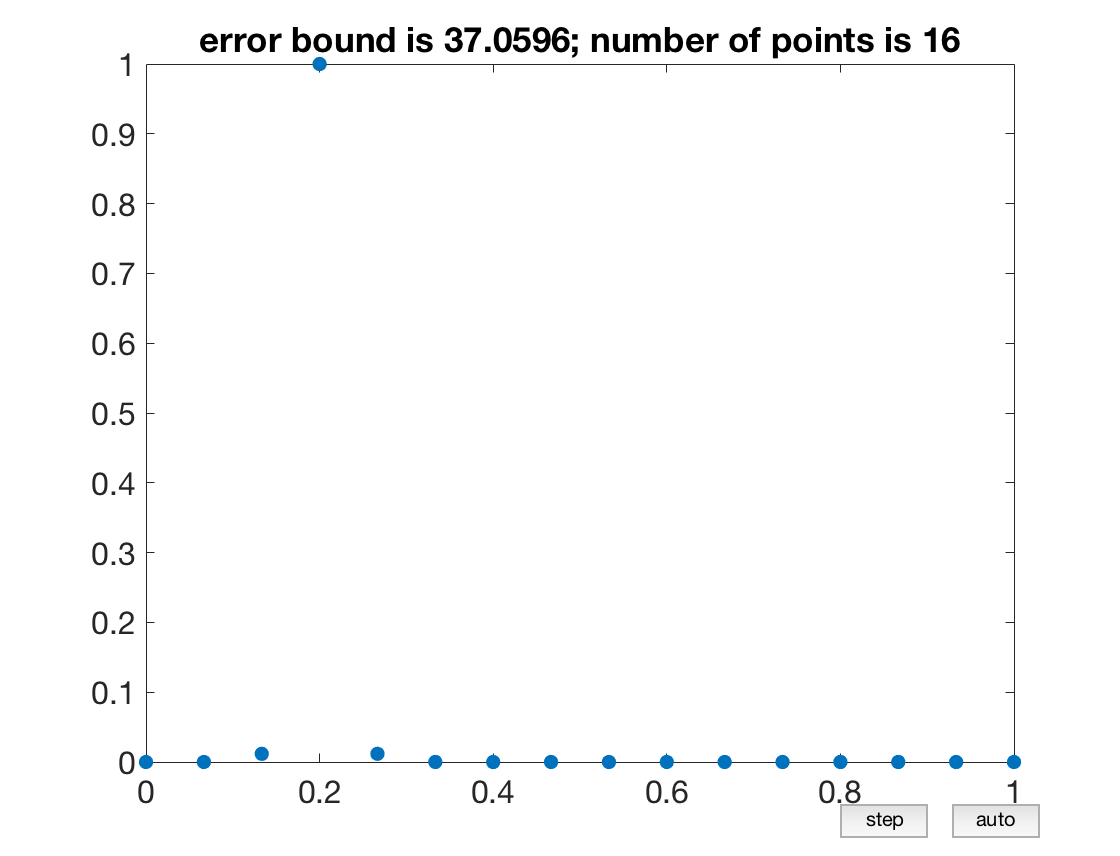
\includegraphics [width=4in]{localgui1.png}

\end{par} \vspace{1em}
\begin{par}
Step 2: add points to the peaky part:
\end{par} \vspace{1em}
\begin{par}

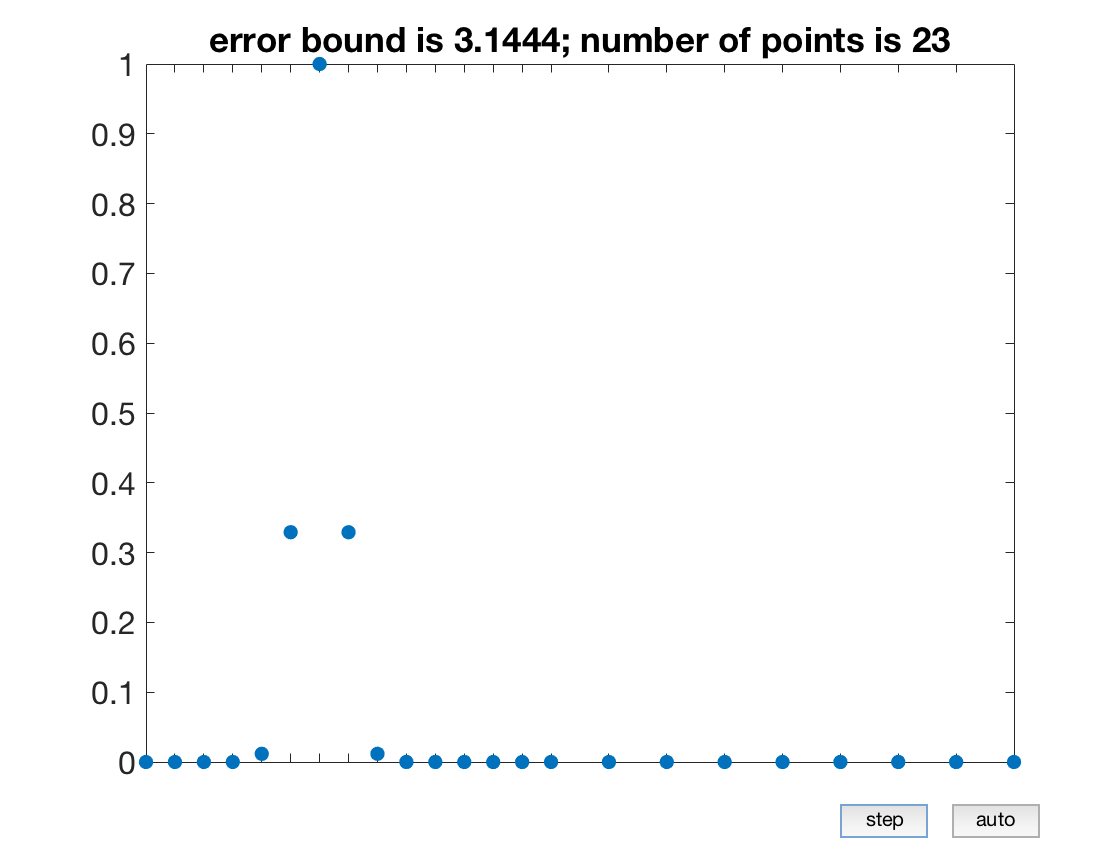
\includegraphics [width=4in]{localgui2.png}

\end{par} \vspace{1em}
\begin{par}
Step 6: after serveral iterations, the approximation error almost meets the given tolerance:
\end{par} \vspace{1em}
\begin{par}

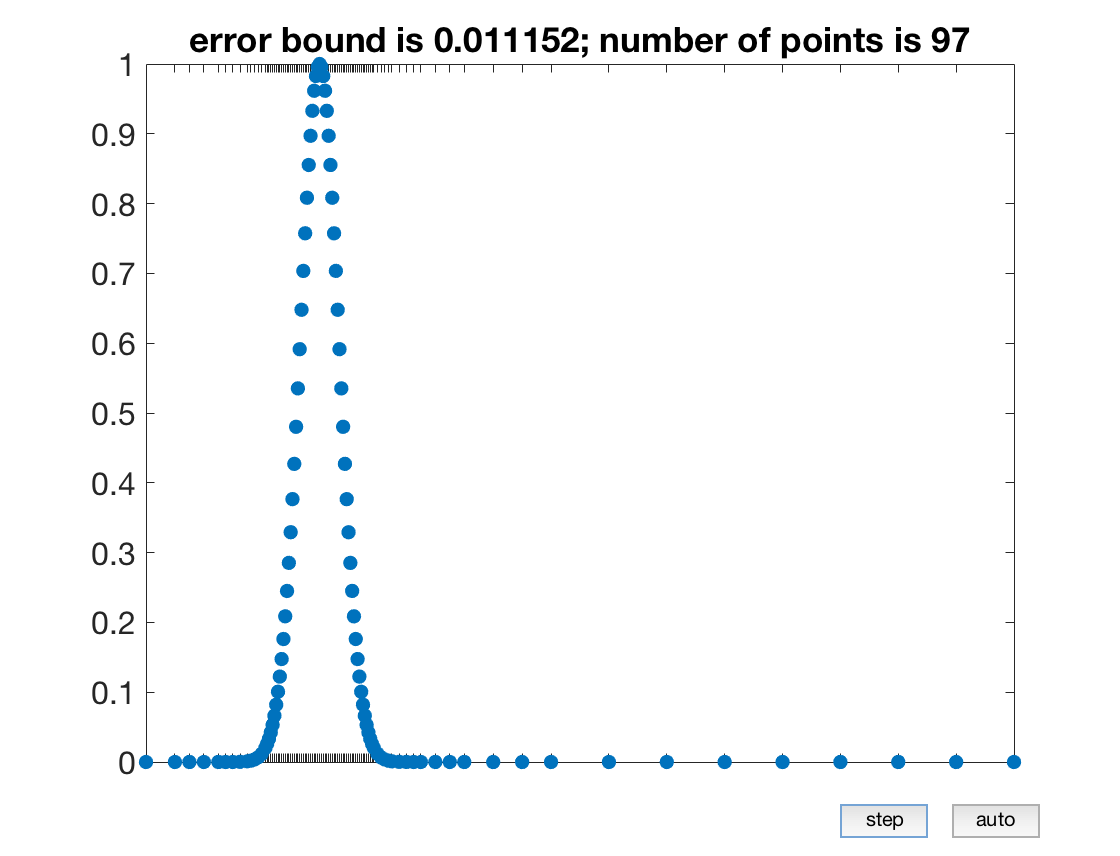
\includegraphics [width=4in]{localgui6.png}

\end{par} \vspace{1em}
\begin{par}
Step 7: the error tolerance is reached:
\end{par} \vspace{1em}
\begin{par}

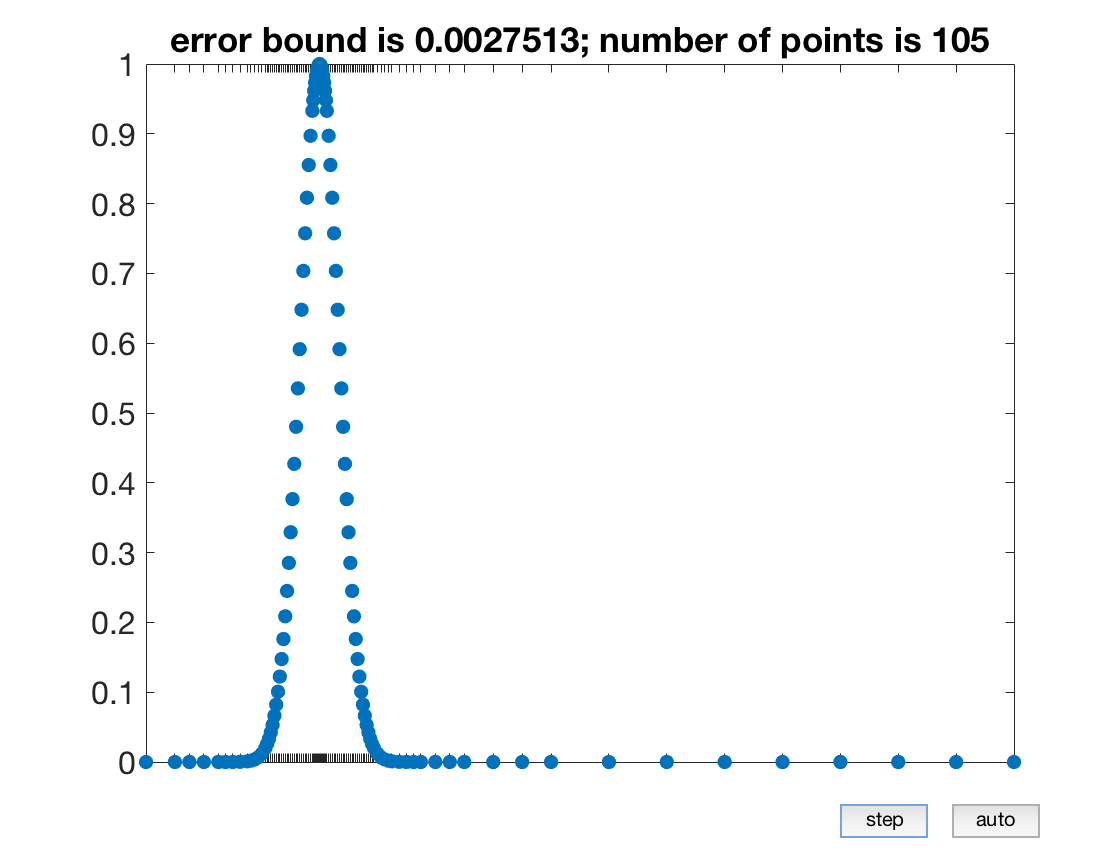
\includegraphics [width=4in]{localgui7.png}

\end{par} \vspace{1em}
\begin{par}
This process can also be reproduced by the following command: funappx\_g\_gui(@(x) exp(-1000*(x-0.2).\^{}2),0,1,1e-2,15,15);
\end{par} \vspace{1em}


\subsection*{References}

\begin{par}
[1] Sou-Cheng T. Choi, Yuhan Ding, Fred J.Hickernell, Xin Tong, "Local     Adaption for Approximation and Minimization of Univariate Functions,"     \textit{Journal of Complexity} 40, pp. 17-33, 2017.
\end{par} \vspace{1em}
\begin{par}
[2] Sou-Cheng T. Choi, Yuhan Ding, Fred J. Hickernell, Lan Jiang, Lluis     Antoni Jimenez Rugama, Da Li, Jagadeeswaran Rathinavel, Xin Tong, Kan     Zhang, Yizhi Zhang, and Xuan Zhou, GAIL: Guaranteed Automatic     Integration Library (Version 2.3.1) [MATLAB Software], 2020. Available     from \begin{verbatim}http://gailgithub.github.io/GAIL_Dev/\end{verbatim}
\end{par} \vspace{1em}


\subsection*{Demos for funmin\_g}

\begin{par}

\end{par} \vspace{1em}
\begin{par}

\end{par} \vspace{1em}


\subsection*{Find the minimum of a highly oscillating curve using \textbf{funmin\_g}}



\subsection*{Function definition}

\begin{par}
Define a highly oscillating function as follows:
\end{par} \vspace{1em}
\begin{par}
\ensuremath{\backslash}[ f(x) = \ensuremath{\backslash}sin (10 \ensuremath{\backslash}pi x\^{}4 ) - x \ensuremath{\backslash}]
\end{par} \vspace{1em}
\begin{verbatim}
close all; clearvars; format compact; format short;
f = @(x) sin(10*pi*x.^4)-x;
\end{verbatim}


\subsection*{Function minimization}

\begin{par}
We use \textbf{funmin\_g} to approximate \ensuremath{\backslash}(f\ensuremath{\backslash}) over the interval \ensuremath{\backslash}([a,b]\ensuremath{\backslash}), where \ensuremath{\backslash}(a = 0\ensuremath{\backslash}) and \ensuremath{\backslash}(b = 2\ensuremath{\backslash}) with default parameter values:
\end{par} \vspace{1em}
\begin{verbatim}
a = 0; b = 2;
[fmin,outmin] = funmin_g(f, a, b);
\end{verbatim}


\subsection*{Plots of the function and its minimum}

\begin{par}
We plot \ensuremath{\backslash}(f(x)\ensuremath{\backslash}) and the approximate minimum returned by \textbf{funmin\_g} below. It is obvious that the approximation is not satisfactory. We compute the error by comparing to the true minimum returned by the Mathematica command, \texttt{N[Minimize[\{Sin[10 Pi x\^{}4] - x, 0 \ensuremath{<}= x \ensuremath{<}= 2\}, \{x\}],15]}.  The reason is probably that this function is not contained in the cone of functions sufficient for successful function minimization.
\end{par} \vspace{1em}
\begin{verbatim}
funmin_g_demo(fmin,outmin)
truefmin=-2.99843616266006;
truexmin=1.99843665971919;
max_abs_error = max(abs(truefmin-fmin))
\end{verbatim}

        \color{lightgray} \begin{verbatim}max_abs_error =
    0.0728
\end{verbatim} \color{black}
    
\includegraphics [width=4in]{gail_ug2_3_06.eps}


\subsection*{A fix}

\begin{par}
We can widen the cone by increasing the number of initial points given to \textbf{funmin\_g}.
\end{par} \vspace{1em}
\begin{verbatim}
inparam.a = a;
inparam.b = b;
inparam.ninit = 1000;
inparam.nmax = inparam.ninit*10;
[fmin2,outmin2] = funmin_g(f, inparam);

funmin_g_demo(fmin2,outmin2)

max_abs_error = max(abs(truefmin-fmin2))
\end{verbatim}

        \color{lightgray} \begin{verbatim}max_abs_error =
   9.3413e-09
\end{verbatim} \color{black}
    
\includegraphics [width=4in]{gail_ug2_3_07.eps}


\subsection*{References}

\begin{par}
[1] Sou-Cheng T. Choi, Yuhan Ding, Fred J.Hickernell, Xin Tong, "Local     Adaption for Approximation and Minimization of Univariate Functions,"   \textit{Journal of Complexity} 40, pp. 17-33, 2017.
\end{par} \vspace{1em}
\begin{par}
[2] Sou-Cheng T. Choi, Yuhan Ding, Fred J. Hickernell, Lan Jiang, Lluis     Antoni Jimenez Rugama, Da Li, Jagadeeswaran Rathinavel, Xin Tong, Kan     Zhang, Yizhi Zhang, and Xuan Zhou, GAIL: Guaranteed Automatic     Integration Library (Version 2.3.1) [MATLAB Software], 2020. Available     from \begin{verbatim}http://gailgithub.github.io/GAIL_Dev/\end{verbatim}
\end{par} \vspace{1em}


\subsection*{Compare \textbf{funmin\_g} with \textbf{fminbnd}}

\begin{par}
Author: Xin Tong, July 2017
\end{par} \vspace{1em}


\subsection*{Function definition}

\begin{par}
Define a function with two minima as follows:
\end{par} \vspace{1em}
\begin{par}
\ensuremath{\backslash}[ f(x) = -5 \ensuremath{\backslash}exp(-100(x-0.2)\^{}2) - \ensuremath{\backslash}exp(-100(x-1)\^{}2). \ensuremath{\backslash}]
\end{par} \vspace{1em}
\begin{verbatim}
close all; clearvars; format compact; format short;
f = @(x) -5*exp((-100*(x-0.2).^2))-exp((-100.*(x-1).^2));
\end{verbatim}


\subsection*{Function minimization}

\begin{par}
We use \textbf{funmin\_g} to find the minimum of \ensuremath{\backslash}(f\ensuremath{\backslash}) over the interval \ensuremath{\backslash}([a,b]\ensuremath{\backslash}), where \ensuremath{\backslash}(a = 0\ensuremath{\backslash}) and \ensuremath{\backslash}(b = 1.5\ensuremath{\backslash}):
\end{par} \vspace{1em}
\begin{verbatim}
a = 0;
b = 1.5;
[fmin,out ] = funmin_g(f,a,b);
[xval,fval] = fminbnd(f,a,b);
\end{verbatim}


\subsection*{Plot of the function and minima}

\begin{par}
We plot \ensuremath{\backslash}(f(x)\ensuremath{\backslash}) and the global minimum value  returned by \textbf{funmin\_g} and a local minimum by \textbf{fminbnd} below:
\end{par} \vspace{1em}
\begin{verbatim}
figure;
x = a:1e-6:b;
fminvec = fmin.*ones(size(x));
plot(x,f(x),'r-',out.intervals,[fmin,fmin],'go',xval,fval,'b*');
ylim([-6 1])
xlabel('$x$','interpreter','latex')
h_legend=legend('$f(x)$','funmin\_g','fminbnd');
set(h_legend,'interpreter','latex');
\end{verbatim}

\includegraphics [width=4in]{gail_ug2_3_08.eps}


\subsection*{References}

\begin{par}
[1] Sou-Cheng T. Choi, Yuhan Ding, Fred J. Hickernell, Xin Tong, "Local     Adaption for Approximation and Minimization of Univariate Functions,"     \textit{Journal of Complexity} 40, pp. 17-33, 2017.
\end{par} \vspace{1em}
\begin{par}
[2] Sou-Cheng T. Choi, Yuhan Ding, Fred J. Hickernell, Lan Jiang, Lluis     Antoni Jimenez Rugama, Da Li, Jagadeeswaran Rathinavel, Xin Tong, Kan     Zhang, Yizhi Zhang, and Xuan Zhou, GAIL: Guaranteed Automatic     Integration Library (Version 2.3.1) [MATLAB Software], 2020. Available     from \begin{verbatim}http://gailgithub.github.io/GAIL_Dev/\end{verbatim}
\end{par} \vspace{1em}


\subsection*{Demos for integral\_g}

\begin{par}

\end{par} \vspace{1em}


\subsection*{Integrate a spiky function using \textbf{integral\_g}}

\begin{par}
Authors:  Fred Hickernell and Sou-Cheng Choi, August 2017
\end{par} \vspace{1em}


\subsection*{Function definition}

\begin{par}
This example is taken from [1], where a function is defined on \ensuremath{\backslash}( [0,1] \ensuremath{\backslash}) with twelve spikes.
\end{par} \vspace{1em}
\begin{verbatim}
close all; clear all; format compact; format short e;
[~,~,MATLABVERSION] = GAILstart(false);

xquad = 0.13579; %number used by quad to split interval into three parts
xleft = [0 xquad/2 xquad 3*xquad/2 2*xquad];
xctr = [2*xquad 1/4+xquad 1/2 3/4-xquad 1-2*xquad];
xrght = [1-2*xquad 1-3*xquad/2 1-xquad 1-xquad/2 1];
xall = [xleft xctr(2:5) xrght(2:5)]';
nnode = length(xall);

fbump = @(x) 4^3*((x.*(1-x)).^3).*((x>=0)&(x<=1)); %one bump
xplot = (0:0.002:1)'; %points to plot
spikyfun = @(x) foolfunmaker(x, @(x,c) fbump((x-c(1))/c(2)),...
    ones(nnode-1,1), [xall(1:nnode-1) diff(xall)]);
\end{verbatim}


\subsection*{Plot of the spiky function}

\begin{par}
In the following, we plot \ensuremath{\backslash}(f(x)\ensuremath{\backslash}) and show the data sampling points picked by MATLAB's built-in integration function \textbf{quad}, which explains why \textbf{quad} essentially gives the answer zero for our spiky function:
\end{par} \vspace{1em}
\begin{verbatim}
figure;
h = plot(xplot,spikyfun(xplot), 'k-', xall, zeros(nnode,1), 'k.');
axis([0 1 -0.3 1.1])
set(gca,'Ytick',-0.2:0.2:1)
legend(h,{'$f$','data'},'location','southeast')
\end{verbatim}

\includegraphics [width=4in]{gail_ug2_3_09.eps}


\subsection*{Integral approximation}

\begin{par}
We use MATLAB built-in functions and \textbf{integral\_g} [2] from GAIL [3] to integrate \ensuremath{\backslash}(f\ensuremath{\backslash}) over the unit interval:
\end{par} \vspace{1em}
\begin{verbatim}
a = 0;
b = 1;
abstol = 1e-11;
if MATLABVERSION >= 8,
    MATintegralspiky = integral(spikyfun,a,b,'AbsTol',abstol)
end
MATquadspiky = quad(spikyfun,a,b,abstol)
MATgailspiky = integral_g(spikyfun,a,b,abstol)
\end{verbatim}

        \color{lightgray} \begin{verbatim}MATintegralspiky =
   4.5714e-01
MATquadspiky =
   2.7021e-44
MATgailspiky =
   4.5714e-01
\end{verbatim} \color{black}
    

\subsection*{Compute approximation errors}

\begin{par}
The true integral value of the spiky function is \ensuremath{\backslash}(16/35\ensuremath{\backslash}). The following code computes absolute errors from the above approximation methods. Only \textbf{integral\_g} achieves the required accuracy with respect to the absolute tolerance of \ensuremath{\backslash}( 10\^{}\{-11\} \ensuremath{\backslash}) in this example.
\end{par} \vspace{1em}
\begin{verbatim}
integralspiky = 16/35;
if MATLABVERSION >= 8,
  abs_errors = abs(integralspiky - [MATintegralspiky, MATquadspiky, MATgailspiky])
else
  abs_errors = abs(integralspiky - [MATquadspiky, MATgailspiky])
end
if_meet_abstol = (abs_errors < abstol)
\end{verbatim}

        \color{lightgray} \begin{verbatim}abs_errors =
   6.1854e-10   4.5714e-01   2.2204e-16
if_meet_abstol =
  1�3 logical array
   0   0   1
\end{verbatim} \color{black}
    

\subsection*{References}

\begin{par}
[1] Nick Clancy, Yuhan Ding, Caleb Hamilton, Fred J. Hickernell, and     Yizhi Zhang, "The Cost of Deterministic, Adaptive, Automatic     Algorithms: Cones, Not Balls," Journal of Complexity 30, pp. 21-45,     2014.
\end{par} \vspace{1em}
\begin{par}
[2] Fred J. Hickernell, Martha Razo, and Sunny Yun, "Reliable Adaptive     Numerical Integration", 2015+, working.
\end{par} \vspace{1em}
\begin{par}
[3] Sou-Cheng T. Choi, Yuhan Ding, Fred J. Hickernell, Lan Jiang, Lluis     Antoni Jimenez Rugama, Da Li, Jagadeeswaran Rathinavel, Xin Tong, Kan     Zhang, Yizhi Zhang, and Xuan Zhou, GAIL: Guaranteed Automatic     Integration Library (Version 2.3.1) [MATLAB Software], 2020. Available     from \begin{verbatim}http://gailgithub.github.io/GAIL_Dev/\end{verbatim}
\end{par} \vspace{1em}


\subsection*{Demos for meanMC\_g}

\begin{par}
\begin{verbatim}html\end{verbatim} \begin{verbatim}href="count_success.html">Demo for meanMC_g</a\end{verbatim} \begin{verbatim}/html\end{verbatim}\%\% Counting the success rate of meanMC\_g Authors: Lan Jiang and Sou-Cheng Choi, July 2017
\end{par} \vspace{1em}
\begin{par}
Define an integration problem as follows:
\end{par} \vspace{1em}
\begin{par}
$$I = \int_0^1 x^2 dx.$$
\end{par} \vspace{1em}
\begin{par}
The analytical solution is \ensuremath{\backslash}(\ensuremath{\backslash}tfrac\{1\}\{3\}\ensuremath{\backslash}). If we use \textbf{meanMC\_g} to estimate the integral with \ensuremath{\backslash}(1000\ensuremath{\backslash}) replications, we expect the success rate to be bigger than or equal to \texttt{(1 - alpha)}.
\end{par} \vspace{1em}
\begin{verbatim}
success = 0;
n = 1000;
in_param.reltol = 0; in_param.abstol = 1e-3;
in_param.alpha = 0.05; Yrand = @(n) rand(n,1).^2;
exactsol = 1/3;
for i = 1:n,
    tmu = meanMC_g(Yrand,in_param);
    check = abs(exactsol-tmu) < 1e-3;
    if check == 1,
        success = success + 1;
    end
end
disp(['Over ' num2str(n) ' replications, there are ' num2str(success) ' successes.'])
disp(['The success rate is ' num2str(success/n) ', which is larger than '...
    num2str(1-in_param.alpha) '.'])
\end{verbatim}

        \color{lightgray} \begin{verbatim}Over 1000 replications, there are 1000 successes.
The success rate is 1, which is larger than 0.95.
\end{verbatim} \color{black}
    

\subsection*{Demos for cubMC\_g}

\begin{par}
\begin{verbatim}html\end{verbatim} \begin{verbatim}href="demo_normal_probabilities.html">Computing normal probabilities</a\end{verbatim} \begin{verbatim}/html\end{verbatim}\%\% Demos for cubSobol\_g
\end{par} \vspace{1em}
\begin{par}

\end{par} \vspace{1em}


\subsection*{Estimation of normal probabilities by \textbf{cubSobol\_g} and \textbf{cubMC\_g}}

\begin{par}
Authors: Lluis Antoni Jimenez Rugama and Lan Jiang, August 2017
\end{par} \vspace{1em}
\begin{par}
For \ensuremath{\backslash}(\ensuremath{\backslash}bf\{X\}\ensuremath{\backslash}sim N(\ensuremath{\backslash}bf\{\ensuremath{\backslash}mu\},\ensuremath{\backslash}Sigma)\ensuremath{\backslash}), we will estimate the following probability:
\end{par} \vspace{1em}
\begin{par}
\ensuremath{\backslash}[ P\ensuremath{\backslash}left(\ensuremath{\backslash}bf\{a\} \ensuremath{\backslash}leq \ensuremath{\backslash}bf\{X\} \ensuremath{\backslash}leq \ensuremath{\backslash}bf\{b\} \ensuremath{\backslash}right) = \ensuremath{\backslash}int\_\{\ensuremath{\backslash}bf\{a\}\}\^{}\{\ensuremath{\backslash}bf\{b\}\} \ensuremath{\backslash}frac\{\{\ensuremath{\backslash}rm e\}\^{}\{(\ensuremath{\backslash}bf\{x\}-\ensuremath{\backslash}bf\{\ensuremath{\backslash}mu\})\^{}T \{\ensuremath{\backslash}Sigma\}\^{}\{-1\}(\ensuremath{\backslash}bf\{x\}-\ensuremath{\backslash}bf\{\ensuremath{\backslash}mu\})\}\} \{(2\ensuremath{\backslash}pi)\^{}\{d/2\}\ensuremath{\backslash}left\ensuremath{|}\{\ensuremath{\backslash}Sigma\}\ensuremath{\backslash}right\ensuremath{|}\^{}\{1/2\}\}\ensuremath{\backslash},\{\ensuremath{\backslash}rm d\}\ensuremath{\backslash}bf\{x\}. \ensuremath{\backslash}]
\end{par} \vspace{1em}
\begin{par}
We present three tests, each of which approximates the aforementioned probability using \textbf{cubSobol\_g} and \textbf{cubMC\_g}, which are quasi-Monte Carlo and IID Monte Carlo algorithms in GAIL, respectively. In order to facilitate the computations when $d$ is high (\ensuremath{\tilde{\;}}30), we are going to apply a special transformation of the integrand proposed by Alan Genz.
\end{par} \vspace{1em}


\subsection*{Basic integration parameters set up}

\begin{par}
For all the examples, the dimension of the problem is $d=30$. The user input tolerances are also set up below: \texttt{abstol} is the absolute error tolerance, and \texttt{reltol} the relative error tolerance. When \texttt{reltol} is set to 0, the algorithms use pure absolute error bound, and vice versa. Finally, for simplicity we define the mean of the distribution to be \ensuremath{\backslash}(\ensuremath{\backslash}bf\{\ensuremath{\backslash}mu\}=\ensuremath{\backslash}bf\{0\}\ensuremath{\backslash}):
\end{par} \vspace{1em}
\begin{verbatim}
function demo_normal_probabilities()
\end{verbatim}
\begin{verbatim}
d = 30; % Dimension of the problem
abstol = 1e-3; % User input, absolute error bound
reltol = 0;  % User input, relative error bound
mu = zeros(d,1); % Mean of the distribution
\end{verbatim}


\subsection*{First test: \ensuremath{\backslash}(\ensuremath{\backslash}Sigma=I\_d\ensuremath{\backslash})}

\begin{par}
For this first example, we consider \ensuremath{\backslash}(\ensuremath{\backslash}Sigma=I\_d\ensuremath{\backslash}), and \ensuremath{\backslash}(\ensuremath{\backslash}bf\{b\}=-\ensuremath{\backslash}bf\{a\}=(3.5,\ensuremath{\backslash}dots,3.5)\ensuremath{\backslash}). In this case, the solution of the integral is known so we can verify that the error conditions are met:
\end{par} \vspace{1em}
\begin{verbatim}
Sigma = eye(d); % We set the covariance matrix to the identity
factor = 3.5;
hyperbox = [-factor*ones(1,d) ; factor*ones(1,d)]; % We define the integration limits
exactsol = (gail.stdnormcdf(factor)-gail.stdnormcdf(-factor))^d; % Exact integral solution

% Solution approx_prob and integration output parameters in out_param
[approx_prob,out_param] = multi_normcdf_cubMC(hyperbox,mu,Sigma,abstol,reltol);
disp('Test 1.1: cubMC_g')
disp(['Estimated probability with cubMC_g is: ' num2str(approx_prob)])
disp(['The algorithm took ' num2str(out_param.time) ' seconds and '...
    num2str(out_param.ntot) ' points.'])
disp(['Real error is ' ...
    num2str(abs(exactsol-approx_prob))...
    ' which is less than the user input tolerance '...
    num2str(gail.tolfun(abstol,reltol,1,exactsol,'max')) '.'])

% Solution approx_prob and integration output parameters in out_param
[approx_prob,out_param] = multi_normcdf_cubSobol(hyperbox,mu,Sigma,abstol,reltol);
disp('Test 1.2: cubSobol_g')
disp(['Estimated probability with cubSobol_g is: ' num2str(approx_prob)])
disp(['The algorithm took ' num2str(out_param.time) ' seconds and '...
    num2str(out_param.n) ' points.'])
disp(['Real error is ' ...
    num2str(abs(exactsol-approx_prob))...
    ' which is less than the user input tolerance '...
    num2str(gail.tolfun(abstol,reltol,1,exactsol,'max')) '.'])
\end{verbatim}


\subsection*{Second test: \ensuremath{\backslash}(\ensuremath{\backslash}Sigma=0.4I\_d + 0.6\ensuremath{\backslash}bf\{1\}\ensuremath{\backslash}bf\{1\}\^{}T\ensuremath{\backslash})}

\begin{par}
For this second example, we consider \ensuremath{\backslash}(\ensuremath{\backslash}Sigma=0.4I\_d + 0.6\ensuremath{\backslash}bf\{1\}\ensuremath{\backslash}bf\{1\}\^{}T\ensuremath{\backslash}) (\ensuremath{\backslash}(1\ensuremath{\backslash}) on the diagonal, \ensuremath{\backslash}(0.6\ensuremath{\backslash}) off the diagonal), \ensuremath{\backslash}(\ensuremath{\backslash}bf\{a\}=(-\ensuremath{\backslash}infty,\ensuremath{\backslash}dots,-\ensuremath{\backslash}infty)\ensuremath{\backslash}), and \ensuremath{\backslash}(\ensuremath{\backslash}bf\{b\}=\ensuremath{\backslash}sqrt\{d\}(U\_1,\ensuremath{\backslash}dots,U\_d)\ensuremath{\backslash}) (\ensuremath{\backslash}(\ensuremath{\backslash}bf\{b\}\ensuremath{\backslash}) is chosen randomly). The solution for this integral is known too so we can verify the real error:
\end{par} \vspace{1em}
\begin{verbatim}
sig = 0.6;
Sigma = sig*ones(d,d); Sigma(1:d+1:d*d) = 1; % set the covariance matrix
hyperbox = [-Inf*ones(1,d) ; sqrt(d)*rand(1,d)]; % define the integration limits
exactsol = integral(@(t)MVNPexact(t,hyperbox(2,:),sig),...
    -inf, inf,'Abstol',1e-8,'RelTol',1e-8)/sqrt(2*pi);

% Solution approx_prob and integration output parameters in out_param
[approx_prob,out_param] = multi_normcdf_cubMC(hyperbox,mu,Sigma,abstol,reltol);
disp('Test 2.1: cubMC_g')
disp(['Estimated probability with cubMC_g is: ' num2str(approx_prob)])
disp(['The algorithm took ' num2str(out_param.time) ' seconds and '...
    num2str(out_param.ntot) ' points.'])
disp(['Real error is ' ...
    num2str(abs(exactsol-approx_prob))...
    ' which is less than the user input tolerance '...
    num2str(gail.tolfun(abstol,reltol,1,exactsol,'max')) '.'])

% Solution approx_prob and integration output parameters in out_param
[approx_prob,out_param] = multi_normcdf_cubSobol(hyperbox,mu,Sigma,abstol,reltol);
disp('Test 2.2: cubSobol_g')
disp(['Estimated probability with cubSobol_g is: ' num2str(approx_prob)])
disp(['The algorithm took ' num2str(out_param.time) ' seconds and '...
    num2str(out_param.n) ' points.'])
disp(['Real error is ' ...
    num2str(abs(exactsol-approx_prob))...
    ' which is less than the user input tolerance '...
    num2str(gail.tolfun(abstol,reltol,1,exactsol,'max')) '.'])
\end{verbatim}


\subsection*{Third test: \ensuremath{\backslash}(\ensuremath{\backslash}Sigma=0.4I\_d + 0.6\ensuremath{\backslash}bf\{1\}\ensuremath{\backslash}bf\{1\}\^{}T\ensuremath{\backslash})}

\begin{par}
For this last example, we consider the same covariance matrix in the second test but the upper and lower limits are different, \ensuremath{\backslash}(\ensuremath{\backslash}bf\{a\}=-d/3(U\_1,\ensuremath{\backslash}dots,U\_d)\ensuremath{\backslash}), and \ensuremath{\backslash}(\ensuremath{\backslash}bf\{b\}=d/3(U\_\{d+1\},\ensuremath{\backslash}dots,U\_\{2d\})\ensuremath{\backslash}) (both \ensuremath{\backslash}(\ensuremath{\backslash}bf\{a\}\ensuremath{\backslash}) and \ensuremath{\backslash}(\ensuremath{\backslash}bf\{b\}\ensuremath{\backslash}) are chosen randomly):
\end{par} \vspace{1em}
\begin{verbatim}
hyperbox = [-(d/3)*rand(1,d) ; (d/3)*rand(1,d)]; % We define the integration limits

% Solution approx_prob and integration output parameters in out_param
[approx_prob,out_param] = multi_normcdf_cubMC(hyperbox,mu,Sigma,abstol,reltol);
disp('Test 3.1: cubMC_g')
disp(['Estimated probability with cubMC_g is: ' num2str(approx_prob)])
disp(['The algorithm took ' num2str(out_param.time) ' seconds and '...
    num2str(out_param.ntot) ' points.'])

% Solution approx_prob and integration output parameters in out_param
[approx_prob,out_param] = multi_normcdf_cubSobol(hyperbox,mu,Sigma,abstol,reltol);
disp('Test 3.2: cubSobol_g')
disp(['Estimated probability with cubSobol_g is: ' num2str(approx_prob)])
disp(['The algorithm took ' num2str(out_param.time) ' seconds and '...
    num2str(out_param.n) ' points.'])
\end{verbatim}


\subsection*{Appendix: Auxiliary function definitions}

\begin{par}
The following functions are defined for the above test examples. \texttt{multi\_normcdf\_cubSobol} and \texttt{multi\_normcdf\_cubMC} redefine \textbf{cubSobol\_g} and \textbf{cubMC\_g} respectively for computing normal probabilites based on Alan Genz's transformation. \texttt{f} is the function resulting from applying Alan Genz's transform that is called in either \textbf{cubSobol\_g} or \textbf{cubMC\_g}.
\end{par} \vspace{1em}
\begin{verbatim}
function [p,out, y, kappanumap] = multi_normcdf_cubSobol(hyperbox,mu,Sigma,abstol,reltol)
% Using cubSobol_g, multi_normcdf_cubMC computes the cumulative
% distribution function of the multivariate normal distribution with mean
% mu, covariance matrix Sigma and within the region defined by hyperbox.
hyperbox = bsxfun(@minus, hyperbox, mu');
C = chol(Sigma)'; d = size(C,1);
a = hyperbox(1,1)/C(1,1); b = hyperbox(2,1)/C(1,1);
s = gail.stdnormcdf(a); e = gail.stdnormcdf(b);
[p, out, y, kappanumap] = cubSobol_g(...
    @(x) f(s,e,hyperbox,x,C), [zeros(1,d-1);ones(1,d-1)],...
    'uniform',abstol,reltol);
end

function [Q,param] = multi_normcdf_cubMC(hyperbox,mu,Sigma,abstol,reltol)
% Using cubMC_g, multi_normcdf_cubMC computes the cumulative distribution
% function of the multivariate normal distribution with mean mu, covariance
% matrix Sigma and within the region defined by hyperbox.
hyperbox = bsxfun(@minus, hyperbox, mu');
C = chol(Sigma)'; d = size(C,1);
a = hyperbox(1,1)/C(1,1); b = hyperbox(2,1)/C(1,1);
s = gail.stdnormcdf(a); e = gail.stdnormcdf(b);
[Q,param] = cubMC_g(...
    @(x) f(s,e,hyperbox,x,C), [zeros(1,d-1);ones(1,d-1)],...
    'uniform',abstol,reltol);
end

function f_eval = f(s,e,hyperbox,w,C)
% This is the integrand resulting from applying Alan Genz's transformation,
% which is recursively defined.
f_eval = (e-s)*ones(size(w,1),1);
aux = ones(size(w,1),1);
y = [];
for i = 2:size(hyperbox,2);
    y = [y gail.stdnorminv(s+w(:,i-1).*(e-s))];
    aux = sum(bsxfun(@times,C(i,1:i-1),y),2);
    a = (hyperbox(1,i)-aux)/C(i,i);
    b = (hyperbox(2,i)-aux)/C(i,i);
    s = gail.stdnormcdf(a);
    e = gail.stdnormcdf(b);
    f_eval = f_eval .* (e-s);
end
end

function MVNPfunvalfinal = MVNPexact(t,b,sig)
% MVNPexact calculates the true solution of multivariate normal probability
% when the covariance matrix is in a special form: diagonal is 1 and off
% diagonal elements are all the same.
%
% b   - the upper limits of the integral with size 1 x d
% sig - the off diagonal element
% dim - the dimension of the integral
% t   - the variable
MVNPfunval = (gail.stdnormcdf((b(1)+sqrt(sig)*t)/sqrt(1-sig)));
dim =  length(b);
for i =2:dim
    MVNPfunval= MVNPfunval.*(gail.stdnormcdf((b(i)+sqrt(sig)*t)/sqrt(1-sig)));
    %i=i+100;
end
MVNPfunvalfinal = MVNPfunval.*exp(-t.^2/2);
end
\end{verbatim}
\begin{verbatim}
end
\end{verbatim}


\subsection*{References}

\begin{par}
[1] Fred J. Hickernell, Lluis Antoni Jimenez Rugama "Reliable adaptive     cubature using digital sequences", Monte Carlo and Quasi-Monte Carlo     Methods: MCQMC, Leuven, Belgium, April 2014 (R. Cools and D. Nuyens,     eds.), Springer Proceedings in Mathematics and Statistics, vol. 163,     Springer-Verlag, Berlin, 2016, arXiv:1410.8615 [math.NA], pp.     367-383.
\end{par} \vspace{1em}
\begin{par}
[2] Fred J. Hickernell, Lan Jiang, Yuewei Liu, and Art B. Owen,     "Guaranteed conservative fixed width confidence intervals via Monte     Carlo sampling," Monte Carlo and Quasi-Monte Carlo Methods 2012     (J. Dick, F. Y. Kuo, G. W. Peters, and I. H. Sloan, eds.),     Springer-Verlag, Berlin, pp. 105-128, 2014.
\end{par} \vspace{1em}
\begin{par}
[3] Sou-Cheng T. Choi, Yuhan Ding, Fred J. Hickernell, Lan Jiang, Lluis     Antoni Jimenez Rugama, Da Li, Jagadeeswaran Rathinavel, Xin Tong, Kan     Zhang, Yizhi Zhang, and Xuan Zhou, GAIL: Guaranteed Automatic     Integration Library (Version 2.3.1) [MATLAB Software], 2020. Available     from \begin{verbatim}http://gailgithub.github.io/GAIL_Dev/\end{verbatim}
\end{par} \vspace{1em}
\begin{par}
[4] Lan Jiang, Guaranteed Adaptive Monte Carlo Methods for Estimating     Means of Random Variables, PhD Thesis, Illinois Institute of     Technology, 2016.
\end{par} \vspace{1em}



\end{document}
    
